% !TeX spellcheck = en_US
%%% The main file. It contains definitions of basic parameters and includes all other parts.

%% Settings for single-side (simplex) printing
% Margins: left 40mm, right 25mm, top and bottom 25mm
% (but beware, LaTeX adds 1in implicitly)
%\documentclass[12pt,a4paper]{report}
%\setlength\textwidth{145mm}
%\setlength\textheight{247mm}
%\setlength\oddsidemargin{15mm}
%\setlength\evensidemargin{15mm}
%\setlength\topmargin{0mm}
%\setlength\headsep{0mm}
%\setlength\headheight{0mm}
% \openright makes the following text appear on a right-hand page
%\let\openright=\clearpage

% set fonts
%\renewcommand{\ttdefault}{Lucida Sans Typewriter}

%% Settings for two-sided (duplex) printing
 \documentclass[12pt,a4paper,twoside,openright]{report}
 \setlength\textwidth{145mm}
 \setlength\textheight{247mm}
 \setlength\oddsidemargin{14.2mm}
 \setlength\evensidemargin{0mm}
 \setlength\topmargin{0mm}
 \setlength\headsep{0mm}
 \setlength\headheight{0mm}
 \let\openright=\cleardoublepage

%% Generate PDF/A-2u
\usepackage[a-2u]{pdfx}

%% Character encoding: usually latin2, cp1250 or utf8:
\usepackage[utf8]{inputenc}

%% Prefer Latin Modern fonts
\usepackage{lmodern}

%% Further useful packages (included in most LaTeX distributions)
\usepackage{amsmath}        % extensions for typesetting of math
\usepackage{mathtools}
\usepackage{amsfonts}       % math fonts
\usepackage{amsthm}         % theorems, definitions, etc.
\usepackage{bbding}         % various symbols (squares, asterisks, scissors, ...)
\usepackage{bm}             % boldface symbols (\bm)
\usepackage{graphicx}       % embedding of pictures
\usepackage{fancyvrb}       % improved verbatim environment
\usepackage{natbib}         % citation style AUTHOR (YEAR), or AUTHOR [NUMBER]
\usepackage[nottoc]{tocbibind} % makes sure that bibliography and the lists
			    % of figures/tables are included in the table
			    % of contents
\usepackage{dcolumn}        % improved alignment of table columns
\usepackage{booktabs}       % improved horizontal lines in tables
\usepackage{paralist}       % improved enumerate and itemize
\usepackage[usenames]{xcolor}  % typesetting in color

\usepackage{algpseudocode}  % for typeseting algorithms
\usepackage{algorithm}	 	% for typeseting algorithms
\usepackage{physics}        % derivatives

\usepackage{minted}		% syntax highlight
%\usepackage{tcolorbox}	% tools for modifying minted environment
%\usepackage{etoolbox}
%\BeforeBeginEnvironment{minted}{\begin{tcolorbox}}%
%\AfterEndEnvironment{minted}{\end{tcolorbox}}%

\usepackage[american,siunitx]{circuitikz}		% circuit diagrams, use 'american' for US symbols
\usepackage{subcaption}
\usepackage{makecell}	    % line breaks inside table cell
\usepackage{tabu}
\usepackage{longtable}

% libraries for TikZ
\usetikzlibrary{arrows,decorations.markings}
%%% Basic information on the thesis

% Thesis title in English (exactly as in the formal assignment)
\def\ThesisTitle{NextGen SPICE – Electrical Circuit Simulation Library for .NET}
\def\ThesisTitleCz{NextGen SPICE – knihovna pro simulaci elektrických obvodů pro .NET}

% Author of the thesis
\def\ThesisAuthor{Radek Zikmund}

% Year when the thesis is submitted
\def\YearSubmitted{2018}

% Name of the department or institute, where the work was officially assigned
% (according to the Organizational Structure of MFF UK in English,
% or a full name of a department outside MFF)
\def\Department{Department of Distributed and Dependable Systems}

% Is it a department (katedra), or an institute (ústav)?
\def\DeptType{Department}

\def\DeptTypeCz{Katedra}


% Thesis supervisor: name, surname and titles
\def\Supervisor{Mgr. Pavel Ježek, Ph.D.}

% Supervisor's department (again according to Organizational structure of MFF)
\def\SupervisorsDepartment{Department of Distributed and Dependable Systems}
\def\SupervisorsDepartmentCz{Katedra distribuovaných a spolehlivých	systémů}

% Study programme and specialization
\def\StudyProgramme{Computer Science}
\def\StudyBranch{Programming and Software Systems}

% An optional dedication: you can thank whomever you wish (your supervisor,
% consultant, a person who lent the software, etc.)
\def\Dedication{%
	I would like to thank my supervisor \Supervisor{} for his time, patience and the advice he gave me during our consultations. Also, special thanks go to my family, friends and everybody who supported me and helped me during my studies.
}

% Abstract (recommended length around 80-200 words; this is not a copy of your thesis assignment!)
\def\Abstract{%	
	The goal of this thesis was to create an extensible library for simulating electrical circuits for the .NET platform, which could be used in broad contexts like development of educational programs or applications that use evolutionary algorithms to evolve electrical circuits. Our library is inspired by the family of SPICE programs developed at University of California, Berkeley.
	
	The initial version of our library implements transient analysis of electrical circuits and supports basic devices like voltage and current sources, resistors, capacitors, inductors, but also semiconductor diode and BJT transistor devices. Our library is designed in such a way that both new circuit devices and circuit analyses can be added in future versions.
	
	Other features of our library include importing circuits or their parts from industry standard SPICE netlists and the ability to modify circuit parameters during the simulation. In this thesis, we also investigate using the double-double precision type to improve convergence during the simulation.
		
	We also implement a simple SPICE-like console application to allow our simulation library to be used from the command line.
}

% 3 to 5 keywords (recommended), each enclosed in curly braces
\def\Keywords{%
	{Electrical circuit simulation} {SPICE} {.NET} {Library}
}

% Abstract (recommended length around 80-200 words; this is not a copy of your thesis assignment!)
\def\AbstractCz{%
	Cílem této práce bylo vytvořit rozšiřitelnou knihovnu pro simulaci elektrických obvodů pro platformu .NET, která by byla uplatnitelná v širokém kontextu, jako je vývoj výukových programů nebo aplikací využívajících evolučních algoritmů pro evoluci elektrických obvodů. Naše knihovna je inspirována rodinou SPICE programů vyvíjených na Kalifornské univerzitě v Berkeley.
	
	Počáteční verze naší knihovny implementuje transientní analýzu elektrických obvodů a podporuje základní součástky jako zdroje napětí a proudu, rezistory, kondenzátory a cívky, ale také polovodičové diody a BJT transistory. Naše knihovna je navržena takovým způsobem, že je možné v budoucích verzích knihovny přidat jak nové součástky, tak nové typy analýz.
	
	Další vlastnosti naší knihovny zahrnují importování obvodů nebo jejich částí v průmyslově standardním SPICE netlist formátu a možnost upravovat parametry součástek během simulace. V této práci také prověřujeme použití typů s přesností double-double pro zlepšení konvergence během simulace.
	
	Také jsme implementovali jednoduchou SPICE-like konzolovou aplikaci abychom umožnili používání naší simulační knihovny z příkazové řádky.
}

% 3 to 5 keywords (recommended), each enclosed in curly braces
\def\KeywordsCz{%
	{Simulace elektrických obvodů} {SPICE} {.NET} {Knihovna}
}

%% The hyperref package for clickable links in PDF and also for storing
%% metadata to PDF (including the table of contents).
%% Most settings are pre-set by the pdfx package.
\hypersetup{unicode}
\hypersetup{breaklinks=true}

% Definitions of macros (see description inside)
%%% This file contains definitions of various useful macros and environments %%%
%%% Please add more macros here instead of cluttering other files with them. %%%

%%% Minor tweaks of style

% These macros employ a little dirty trick to convince LaTeX to typeset
% chapter headings sanely, without lots of empty space above them.
% Feel free to ignore.
\makeatletter
\def\@makechapterhead#1{
  {\parindent \z@ \raggedright \normalfont
   \Huge\bfseries \thechapter. #1
   \par\nobreak
   \vskip 20\p@
}}
\def\@makeschapterhead#1{
  {\parindent \z@ \raggedright \normalfont
   \Huge\bfseries #1
   \par\nobreak
   \vskip 20\p@
}}
\makeatother

% This macro defines a chapter, which is not numbered, but is included
% in the table of contents.
\def\chapwithtoc#1{
\chapter*{#1}
\addcontentsline{toc}{chapter}{#1}
}

% Draw black "slugs" whenever a line overflows, so that we can spot it easily.
\overfullrule=1mm

%%% Macros for definitions, theorems, claims, examples, ... (requires amsthm package)

\theoremstyle{plain}
\newtheorem{thm}{Theorem}
\newtheorem{lemma}[thm]{Lemma}
\newtheorem{claim}[thm]{Claim}

\theoremstyle{plain}
\newtheorem{defn}{Definition}

\theoremstyle{remark}
\newtheorem*{cor}{Corollary}
\newtheorem*{rem}{Remark}
\newtheorem*{example}{Example}

%%% An environment for proofs

%%% FIXME %%% \newenvironment{proof}{
%%% FIXME %%%   \par\medskip\noindent
%%% FIXME %%%   \textit{Proof}.
%%% FIXME %%% }{
%%% FIXME %%% \newline
%%% FIXME %%% \rightline{$\square$}  % or \SquareCastShadowBottomRight from bbding package
%%% FIXME %%% }

%%% An environment for typesetting of program code and input/output
%%% of programs. (Requires the fancyvrb package -- fancy verbatim.)

\renewcommand{\theFancyVerbLine}{\ttfamily \normalfont \arabic{FancyVerbLine}:} %% bigger line numbers

\DefineVerbatimEnvironment{spicecode}{Verbatim}{fontsize=\footnotesize,frame=single, numbers=left, tabsize=4,commandchars=\\\{\}}

\DefineVerbatimEnvironment{code}{Verbatim}{fontsize=\footnotesize,frame=single, tabsize=4}

\newminted{csharp}{frame=single, linenos, tabsize=4, mathescape=true, fontsize=\footnotesize}
\usemintedstyle{vs} %does not seem to work?

%% macro for coloring of the equations
\makeatletter
\def\mathcolor#1#{\@mathcolor{#1}}
\def\@mathcolor#1#2#3{%
	\protect\leavevmode
	\begingroup
	\color#1{#2}#3%
	\endgroup
}
\makeatother


% environment for algorithms
\newenvironment{alg}[1]
{
	\begin{algorithm}
	\caption{#1}
	\begin{algorithmic}[1]
}
{	
	\end{algorithmic}
	\end{algorithm}
}

% environment for small inline circuit examples
\newenvironment{circuitdev}
{
	\begin{center}	
	\begin{circuitikz}[scale=0.8, font=\footnotesize]
	\draw 
}
{
	;
	\end{circuitikz}
	\end{center}
}

%%% inline quote
\newcommand{\shortquote}[1]{`\textit{#1}'} 

%%% force italics in the quote
\newenvironment{blockquote}
{
	\begin{quotation}
	\itshape
}
{
	\end{quotation}
}



%%% macro for introducing line breaks without hyphenation
\newcommand{\+}{\discretionary{}{}{}}

%%% Asymptotic notaion
\newcommand{\bigO}[1]{\mathcal{O}(#1)}

%%% The field of all real and natural numbers
\newcommand{\R}{\mathbb{R}}
\newcommand{\N}{\mathbb{N}}

%%% Useful operators for statistics and probability
\DeclareMathOperator{\pr}{\textsf{P}}
\DeclareMathOperator{\E}{\textsf{E}\,}
%\DeclareMathOperator{\var}{\textrm{var}}
\DeclareMathOperator{\sd}{\textrm{sd}}

%%% Transposition of a vector/matrix
\newcommand{\T}[1]{#1^\top}

%%% Various math goodies
\newcommand{\goto}{\rightarrow}
\newcommand{\gotop}{\stackrel{P}{\longrightarrow}}
\newcommand{\maon}[1]{o(n^{#1})}
%\newcommand{\abs}[1]{\left|{#1}\right|}
\newcommand{\dint}{\int_0^\tau\!\!\int_0^\tau}
\newcommand{\isqr}[1]{\frac{1}{\sqrt{#1}}}

%%% Various table goodies
\newcommand{\pulrad}[1]{\raisebox{1.5ex}[0pt]{#1}}
\newcommand{\mc}[1]{\multicolumn{1}{c}{#1}}

%%% Macro for red text in to-do sections
\newcommand{\todo}[1]{{\color{red} TODO: [#1]}}


% Title page and various mandatory informational pages
\begin{document}
%%% Title page of the thesis and other mandatory pages

%%% Title page of the thesis

\pagestyle{empty}
\hypersetup{pageanchor=false}
\begin{center}

\centerline{\mbox{
\includegraphics[width=166mm]{../img/logo-en.pdf}}}

\vspace{-8mm}
\vfill

{\bf\Large BACHELOR THESIS}

\vfill

{\LARGE\ThesisAuthor}

\vspace{15mm}

{\LARGE\bfseries\ThesisTitle\par}

\vfill

\Department

\vfill

\begin{tabular}{rl}

Supervisor of the bachelor thesis: & \Supervisor \\
\noalign{\vspace{2mm}}
Study programme: & \StudyProgramme \\
\noalign{\vspace{2mm}}
Study branch: & \StudyBranch \\
\end{tabular}

\vfill

% Zde doplňte rok
Prague \YearSubmitted

\end{center}

\newpage

%%% Here should be a bound sheet included -- a signed copy of the "bachelor
%%% thesis assignment". This assignment is NOT a part of the electronic
%%% version of the thesis. DO NOT SCAN.

%%% A page with a solemn declaration to the bachelor thesis

\openright
\hypersetup{pageanchor=true}
\pagestyle{plain}
\pagenumbering{roman}
\vglue 0pt plus 1fill

\noindent
I declare that I carried out this bachelor thesis independently, and only with the cited
sources, literature and other professional sources.

\medskip\noindent
I understand that my work relates to the rights and obligations under the Act No.~121/2000 Sb.,
the Copyright Act, as amended, in particular the fact that the Charles
University has the right to conclude a license agreement on the use of this
work as a school work pursuant to Section 60 subsection 1 of the Copyright Act.

\vspace{10mm}

\hbox{\hbox to 0.5\hsize{%
In ........ date ............	% FIXME!
\hss}\hbox to 0.5\hsize{%
signature of the author
\hss}}

\vspace{20mm}
\newpage

%%% Mandatory information page of the thesis

\openright

\vbox to 0.5\vsize{
\setlength\parindent{0mm}
\setlength\parskip{5mm}

Title:
\ThesisTitle

Author:
\ThesisAuthor

\DeptType:
\Department

Supervisor:
\Supervisor, \SupervisorsDepartment

Abstract:
\Abstract

Keywords:
\Keywords

\vss}

%\nobreak
\newpage \openright
\vbox to 0.49\vsize{
\setlength\parindent{0mm}
\setlength\parskip{5mm}
	
Název práce:
\ThesisTitleCz
	
Autor:
\ThesisAuthor
	
\DeptTypeCz:
\Department
	
Vedoucí bakalářské práce:
\Supervisor, \SupervisorsDepartmentCz
	
Abstrakt:
\AbstractCz
	
Klíčová slova:
\KeywordsCz
	
\vss}

\newpage

%%% Dedication

\openright

\noindent
\Dedication

\newpage

\openright
\pagestyle{plain}
\pagenumbering{arabic}
\setcounter{page}{1}


%%% A page with automatically generated table of contents of the bachelor thesis

\tableofcontents

%% Set path for pictures
\graphicspath{ {../img/} }
\usemintedstyle{colorful}

%%% Each chapter is kept in a separate file
%\chapter*{Introduction}
\addcontentsline{toc}{chapter}{Introduction}

The process of designing electrical circuits consists of several stages, starting with detailed specification from the customer that provides all necessary requirements,
and ending with a working prototype of the final product. Intermediate stages include prototyping circuits using a construction base commonly referred to as breadboard, which is is often
very slow and for complex integrated circuits even impossible. The task has been made easier with the invention of electrical circuit simulation programs, which allow quick circuit prototyping
without the need of soldering iron.

Today's computers have enough computing capacity that we can consider using evolutionary algorithms to evolve electrical circuit parameters. We can even
use techniques of genetic programming for evolving the circuit's topology \todo{reference some relevant article?}, which is yet another reason why
electrical circuit simulators are very valuable in the electro-technical industry  \todo{Note: inspired from Inside SPICE}.

\section{The Berkeley SPICE}
One of the most successful circuit simulators was the SPICE program developed at EECS Department of the University of California, Berkeley. The name stands for \textbf{S}imulation \textbf{P}rogram with \textbf{I}ntegrated \textbf{C}ircuit \textbf{E}mphasis. The original SPICE1 program was implemented in \todo{Fortran} and was released in 1971. It's popoularity quickly rose and few years later, Berkeley released SPICE2 with many performance improvements and model enhancements.

During the 1980s, Berkeley decided to rewrite SPICE2 into the C programming language to make it better suited to --- at that time increasingly more popular --- UNIX-based operating systems \cite{spice_book}. The resulting SPICE3 was to be superset of SPICE2, but the development was in the end left to handful of students due to the limited financial resources. The first release of SPICE3 was very buggy and was not even backward compatible with SPICE2. It was mainly due to the incompatibility that SPICE3 did not replace SPICE2, because hundreds of commonly used macro-models would have to be rewritten before they could be used in SPICE3 \cite{inside_spice}.

\section{SPICE3 and K\&R C}
The SPICE3 was written in now non-standard C K\&R norm, because the development started years before the first ANSI norm was released in 1990. Due to the nature of the C language, many parts of the simulator are very fragile. Consider following code snippet from last SPICE3 version source code. It contains a function that loads instances of voltage controlled current source devices to the equation matrix. On the very first line of the function, the \todo{code} inModel parameter is cast to pointer to concrete type of the device.

\todo{include source paths?}
\begin{code}
	/*ARGSUSED*/
	int
	VCCSload(inModel,ckt)
	GENmodel *inModel;
	CKTcircuit *ckt;
	/* actually load the current values into the 
	* sparse matrix previously provided 
	*/
	{
		register VCCSmodel *model = (VCCSmodel *)inModel;
		register VCCSinstance *here;
		
		/*  loop through all the source models */
		for( ; model != NULL; model = model->VCCSnextModel ) {
			
			/* loop through all the instances of the model */
			for (here = model->VCCSinstances; here != NULL ;
			here=here->VCCSnextInstance) {
				
				*(here->VCCSposContPosptr) += here->VCCScoeff ;
				*(here->VCCSposContNegptr) -= here->VCCScoeff ;
				*(here->VCCSnegContPosptr) -= here->VCCScoeff ;
				*(here->VCCSnegContNegptr) += here->VCCScoeff ;
			}
		}
		return(OK);
	}
\end{code}

This function is one example of many functions that must exist for each device to be used in SPICE3. Other such functions include methods for model updating and data printing. Such an arrangement can be a source of many hard-to-debug bugs when attempting to extend the circuit simulator.

%
%\begin{code}
%typedef struct sGENmodel {       /* model structure for a resistor */
%	int GENmodType; /* type index of this device type */
%	struct sGENmodel *GENnextModel; /* pointer to next possible model in 
%	* linked list */
%	GENinstance * GENinstances; /* pointer to list of instances that have this
%	* model */
%	IFuid GENmodName;       /* pointer to character string naming this model */
%} GENmodel;
%
%//....
%
%typedef struct sVCCSmodel {       /* model structure for a source */
%	int VCCSmodType;    /* type index of this device type */
%	struct sVCCSmodel *VCCSnextModel;    /* pointer to next possible model 
%	* in linked list */
%	VCCSinstance * VCCSinstances;    /* pointer to list of instances 
%	* that have this model */
%	IFuid VCCSmodName;       /* pointer to character string naming this model */
%} VCCSmodel;
%
%\end{code}
%

%Since the release of SPICE3, many open-source and commercial circuit simulators have been developed. Examples include PSpice, HSpice and LTspice. Most of these modern simulators accept circuit description in a format that is similar the original SPICE program and can therefore make use of the vast amount of existing macro-models.
%
%The main goal of this thesis is implementation of an extensible SPICE-like simulation library in a modern programming language to be used in applications that require circuit simulations. \todo{this seems out of place.}

\section{Nonconvergence due to insufficient numeric precision}

Most of the common circuit simulators use precision type \todo{code environment} double with approximately 15 decimal significant digits precision. This leads to truncation errors while finding the solution of circuit equations with coefficients that differ in more than 15 orders of magnitude. The truncation errors in turn lead to noise in simulator output or in the worst case to nonconvergence of the solution.

Coefficient differences of this magnitude may commonly occur when resistors with very small resistance values are used. Even though this is generally discouraged and avoided for exactly these reasons, such resistors may result from macromodel \todo{use macromodel, or macro-model consistently} construction. \todo{cite } (https://www.edn.com/design/analog/4418707/1/Extended-precision-simulation-cures-SPICE-convergence-problems).
\todo{example of macromodel construction?}

Following figure shows an example circuit for which the double precision is insufficient.

\todo{example circuit figure + plot of expected and actual values}

This thesis therefore also investigates the possibility of using extended precision technique known as double-double in circuit simulations. This method uses two floating point variables $h, l$, one containing the upper half of significant digits and the other the lower half, to represent a single value $h + l$. As opposed to special types like \todo{code} long double in C++, which are implementation defined and often have higher precision only on specialized hardware, this approach uses standard operations available on all common processors. \todo{mention that value is represented as sum of components?}

\section{Goals of this Thesis}
The goal of this thesis is to reimplement a certain subset of SPICE's functionality using C\# .NET. Implementation will be divided into two principal components -- a reusable library for simulating electrical circuicts, and a console application capable of reading SPICE like netlists \todo{just a subset?} and perform analyses using said library.

Emphasis will be given mainly to extensibility and re-usability of the core simulation library. The library will expose an interface for adding new circuit devices and even new analysis types, without the need for the library's source code modification. Therefore, the standalone library could be used in any application that needs simulate electrical circuits.

This thesis will also investigate higher precision technique double-double and it's appropriateness for circuit simulation with respect to runtime and precision.

\subsection{Supported Analysis types}
The library will implement the following analysis types
\begin{itemize}
	\item DC Operating Point Analysis
	\item Transient Analysis
\end{itemize}

\subsection{Supported Devices}
The library will implement at least the following device types for above mentioned analyses.
\begin{itemize}
	\item Ideal resistor
	\item Ideal voltage source
	\item Ideal current source
	\item Ideal inductor
	\item Ideal capacitor
	\item SPICE-like diode model
\end{itemize}


%\part{Introduction}

\chapter{Introduction}

The process of designing electrical circuits consists of several stages, starting with a detailed specification from the customer that provides all necessary requirements, and ending with a working prototype of the final product. Intermediate stages include prototyping circuits using a construction base commonly referred to as a breadboard, which is is often very slow and for complex integrated circuits even impossible. The task has been made easier with the invention of electrical circuit simulation programs, which allow quick circuit prototyping without the need of a soldering iron.

\section{Berkeley SPICE}
One of the most successful circuit simulators is the SPICE program\footnote{The name SPICE stands for Simulation Program with Integrated Circuit Emphasis.} developed at the EECS Department of the University of California, Berkeley. The original SPICE1 program is implemented in the FØRTRAN language and was released in 1971. Its popularity quickly rose and a few years later, Berkeley released SPICE2 with many performance improvements and model enhancements. The SPICE programs developed at Berkeley heavily influenced the development of future circuit simulation software, and we will describe them in more depth in the following sections.

\subsubsection*{Netlists}
Early versions of SPICE did not operate in interactive mode, therefore the input files contained both data and instructions for processing. These input files conventionally have the \texttt{.cir} extension, and the contained circuit description is called a \textit{netlist}. A simple example of netlist is shown on the figure~\ref{fig:example_circuit} on the left, with a schematic of the corresponding circuit on the right. The meaning of individual lines of the netlist is explained in the next paragraph.

\begin{figure}[h]
\centering
\begin{subfigure}{.25\textwidth}
\begin{spicecode}
BRIDGE-T CIRCUIT
*
VBIAS 1 0 12
R1 1 2 10
R2 2 0 10
R3 2 3 5
R4 1 3 5
*
.OP
.END
\end{spicecode}		
	\end{subfigure}\hspace{5mm}
	\begin{subfigure}{.7\textwidth}	
	\centering	
		\begin{circuitdev}
			(0,0) 
			to[V=12<\volt>,invert,a=VBIAS] (3,0) node[label={-90:$1$}]{}
			-- (6,0)
			to[R, l=5<\ohm>, .-*, a=R4] (6,3) node[label={3:$3$}]{}
			to[R, l=5<\ohm>, a=R3] (3,3) node[label={$2$}]{}
			to[R, l=10<\ohm>, a=R2] (0,3)
			-- (0,0)
		
			(3,0) to[R, l=10<\ohm>, a=R1, *-*] (3,3)
			(0,1.5) -- (-0.5,1.5) node[ground]{}
		\end{circuitdev}
\end{subfigure}
	\caption{Example \texttt{.cir} netlist file, reproduced from The SPICE Book \cite{spice_book} and the corresponding circuit schematic}
	\label{fig:example_circuit}
\end{figure}

The netlist in figure~\ref{fig:example_circuit} is divided into three sections, separated by empty comments on lines 2 and 8. The first section of the netlist contains the name of the circuit, then follows a second section with definitions of five devices: one voltage source and four resistors. The type of each device is inferred from the first letter of its name. Each definition contains a list of connected nodes and the value of a source voltage or a resistor's ohmic resistance, respectively. Node 0 is special, because it corresponds to the ground and must be present in every circuit (a detailed description of SPICE netlists syntax and rules for validating the circuit will be presented later in chapter~\ref{chap:spicecode}). In the last section of the file, there is an \texttt{.OP} statement, which instructs the simulator to perform an operating point analysis to find stable values of node voltages of the circuit, and an \texttt{.END} statement denoting the end of the netlist. This syntax for describing electrical circuits became an industry standard during the 1970s, and most modern circuit simulators still recognize it.

When SPICE2 is run with the previously shown netlist file, it first reads all components, checks syntax and topology rules for the circuit, and then runs the operating point analysis -- computes node voltages and current through the \texttt{VBIAS} voltage source. After that, it prints a rather verbose report, as shown in figure~\ref{fig:example_output}. First, a description of the input circuit is repeated back to the user (only part of the description is shown in the figure for brevity, in the top half in grey), then follows a list of node voltages and then currents flowing through voltage sources.

\begin{figure}[h]
	\begin{spicecode}
\color{lightgray}******* 03/19/91 ********* SPICE 2G.6  9/21/84 ********* 06:47:36 *********
	
\color{lightgray}BRIDGE-T CIRCUIT
	
\color{lightgray} ****     CIRCUIT DESCRIPTION

\color{lightgray}***************************************************************************
\color{lightgray}*
\color{lightgray}VBIAS 1 0 12
\color{lightgray}...
\color{lightgray}.END

******* 03/19/91 ********* SPICE 2G.6  9/21/84 ********* 06:47:36 *********

BRIDGE-T CIRCUIT

 ****  SMALL SIGNAL BIAS SOLUTION   TEMPERATURE = 27.000 DEG C
 
***************************************************************************

 NODE    VOLTAGE     NODE    VOLTAGE     NODE    VOLTAGE    NODE   VOLTAGE

(    1)    12.0000  (    2)     8.0000  (    3)    10.0000 

    VOLTAGE SOURCE CURRENTS
    NAME         CURRENT
    
    VBIAS       -8.000E-01
    
    TOTAL POWER DISSIPATION 9.60E+00 WATTS
	\end{spicecode}
	\caption{Output of SPICE2G.6 for the example netlist file, from The SPICE Book \cite{spice_book}}
	\label{fig:example_output}
\end{figure}


\subsubsection*{Macromodels}
One of the most useful features of SPICE is the ability to define custom subcircuits, called \textit{macromodels}, composed from devices already integrated in the simulator, or other macromodels. Circuits can be then decomposed into individual subcircuits, similarly to how a computer program's source code can be decomposed into individual functions. One macromodel can then represent a complex real-life device, e.g. an amplifier, and can be simply reused throughout the whole circuit.

This allows device manufacturers to provide SPICE netlists with macromodels that accurately model their devices. An example of such a manufacturer is Analog Devices, macromodels for their products can be downloaded from their webpage, a screenshot of which is shown in figure~\ref{fig:analog-macromodel-website}. The manufacturer's customers can then use these macromodels in their simulators to model the behavior of a circuit that uses the manufacturer's products.

\begin{figure}[h]
	\centering
	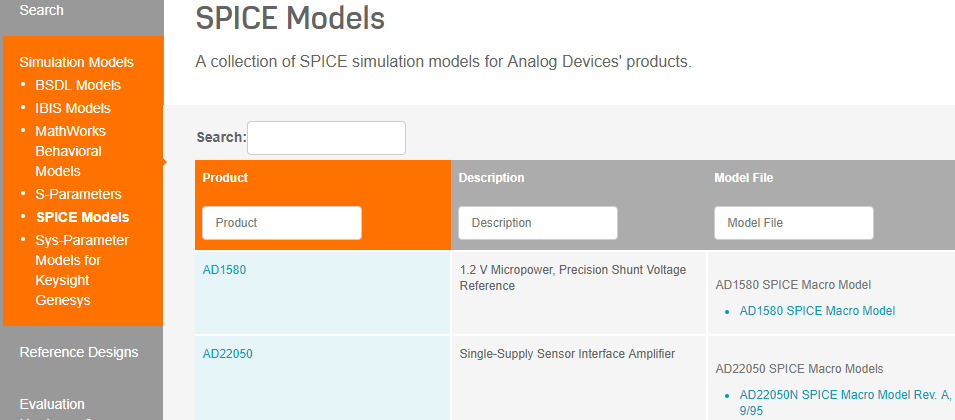
\includegraphics[width=\textwidth]{01-fig-analog-website-macromodels.png}
	\caption{Website of Analog Devices, where SPICE macromodels can be downloaded.}
	\label{fig:analog-macromodel-website}
\end{figure}

Today, vast libraries containing hundreds of SPICE netlists with macromodels exist, and therefore it is a very important feature of any modern circuit simulator to be able to import macromodels from these netlists.

Manufacturer-supplied macromodels are often very complex and the netlists are too long to be shown here. Instead, the use of macromodels is demonstrated on a simple macromodel for an AC coupled amplifier. The netlist description is shown in figure~\ref{fig:example_subcircuit}. A very important part of the definition is the opening \texttt{.SUBCKT} statement, which denotes the start of the subcircuit description, and specifies its name and terminal nodes which will serve as an interface to the outer circuit. After that follows a description of the devices that constitute the macromodel, and finally, the subcircuit definition is ended by an \texttt{.ENDS} statement. The subcircuit in the figure is named ACamplifier and the terminal nodes are 1, 2 and 3. Other nodes (excluding \texttt{0}, which is a global ground node) and all devices used between the \texttt{.SUBCKT} and \texttt{.ENDS} statement are strictly local to the subcircuit and are not visible to the outside circuit.

\begin{figure}[H]
	\centering	
	\begin{subfigure}{.43\textwidth}
	\begin{spicecode}
* external nodes:  in power out
.SUBCKT  ACamplifier 2 1 3
R1 1 4 2K
R2 4 0 500
C1 2 4 10n
Q1 3 4 5 2N2222
Rc 1 3 2K
Re 5 0 1e3
.MODEL 2N2222 NPN 
+ (BF=50 IS=1E-13 VBF=50)
.ENDS
	\end{spicecode}		
\end{subfigure}\hspace{5mm}
\begin{subfigure}{.5\textwidth}	
	\begin{circuitdev}
		(0.3,0) node[circ,label=1]{}
		-- (5.5,0)
		to[R=Rc, a=2<\kilo\ohm>] (5.5,-2)		
		node[npn, label={right:Q1 2N3904}, anchor=C](npn) {}		
		(npn.emitter) node[label=1:5]{}
		to[R=Re, a=1<\milli\ohm>, *-] (5.5, -6) node[ground]{}
		-- (2.5, -6)
		to[R=500<\ohm>, a=R2] (2.5, -3.3)
		-- (2.5,-2.93) node[label=3:4]{}
		-- (npn.base)
		-- (2.5,-2.93) 
		to[R=2<\kilo\ohm>, a=R1] (2.5,0)
		(2.5,-2.93) to[C=10<\nano\farad>, a=C1, *-*]
		(0.3, -2.93) node[label=2]{}
		
		(5.5, -2) -- (6.6,-2) node[circ,label=3]{}
	\end{circuitdev}
\end{subfigure}
\caption{Simple macromodel example for AC coupled amplifier \cite{5spice-subcircuit}, and corresponding circuit schematic, adapted from a 5Spice tutorial by Richard P. Andresen}
\label{fig:example_subcircuit}	
\end{figure}

Such a macromodel can then be used by providing nodes for terminal connections. In a SPICE netlist, a macromodel is represented by a device with a name staring with an X. The actual macromodel to be used is specified as the last argument in the device statement. An example of a circuit that uses the ACamplifier macromodel is shown in figure~\ref{fig:example_subcircuit_call}. The macromodel definition is inlcuded from a separate file, similarly to the \texttt{\#include} preprocessor directive in C or C++. In the actual circuit, the macromodel is represented by the \texttt{XAMP} device. Nodes 3, 2 and 1 are mapped onto the nodes 2, 1 and 3 from the macromodel description.

\begin{figure}[h]
	\centering	
	\begin{subfigure}{.35\textwidth}
		\begin{spicecode}
SUBCIRCUIT CALL EXAMPLE
*
.INCLUDE acamplifier.cir
*
V1 2 0 5
R1 2 3 10
XAMP 3 2 1 ACamplifier
R2 3 0 20
*
.END
		\end{spicecode}		
	\end{subfigure}\hspace{1mm}
	\begin{subfigure}{.61\textwidth}	
		\begin{circuitdev}
			
			(-1,0) to[R=10<\ohm>, a=R1, *-*] (-1, -2.93)
			
			(-2.5,-8.5) to[V=5<\volt>, a=V1, invert]			
			(-2.5,0) -- (-1, 0) node[label={$2 = 1'$}]{}
			-- (4.5,0)
			to[R] (4.5,-2)		
			node[npn, anchor=C](npn) {}		
			(npn.emitter) 
			to[R] (4.5, -6) node[ground]{}
			-- (2.5, -6)
			to[R] (2.5, -3.3)
			-- (2.5,-2.93) 
			-- (npn.base)
			-- (2.5,-2.93)
			to[R] (2.5,0)
			(2.5,-2.93) to[C] (0, -2.93)--
			(-1, -2.93) node[label=270:{$3 = 2'$}]{}
			
			(4.5, -2) -- (6.3,-2) node[circ,label=90:{$1 = 3'$}]{}
			-- (6.3, -8.5) to[R=20<\ohm>, a=R2] (-2.5,-8.5) node[ground]{}	
			;
			\draw[draw=black, very thick, fill=lightgray, fill opacity=0.8] (0.5,0.5) rectangle ++(5,-7.7) ;
			\node at (3,1) {XAMP (ACamplifier)}
		\end{circuitdev}
	\end{subfigure}
	\caption{Illustrative example of circuit that uses macromodel from figure~\ref{fig:example_subcircuit}}
	\label{fig:example_subcircuit_call}	
\end{figure}

\subsubsection*{From SPICE2 to SPICE3}
SPICE2 was not the last SPICE program developed at Berkeley. With the increasingly more popular UNIX-based operating systems, it was possible for programs to be more interactive. Andrei Vladimirescu states in The SPICE Book \cite{spice_book} that SPICE2 was \shortquote{a FORTRAN batch program and was difficult to modify and limited in its potential use of C-shell utilities}. These limitations led Berkeley to start the development of SPICE3 in the C programming language during the 1980s. In addition to more detailed models and improved numerical accuracy, SPICE3 was to support interactive mode, which allowed separating the circuit description from commands for requesting circuit analysis.

Unfortunately, the development was in the end left to a handful of students due to limited financial resources. The first release of SPICE3 was very buggy and was not backward compatible with SPICE2. This was a big problem, because hundreds of commonly used macro-models would have to be rewritten before they could be used in SPICE3. Even though most incompatibility issues were fixed in later releases, SPICE3 did not completely replace SPICE2 and both coexist as two standards for circuit simulations, with the SPICE2 one being a subset of SPICE3 and therefore more portable.

\section{Present-day Situation}
The SPICE programs developed at Berkeley strongly influenced the development of circuit simulators used in industry. Because of the vast existing libraries of SPICE netlist files for various circuits, most circuit simulators either use a syntax which is a superset of the one used in SPICE, or provide some other way of importing circuits from the standard SPICE format.\footnote{Example of a simulator which does not support SPICE syntax directly is QUCS simulator, which provides a tool for transforming the netlist in SPICE format into the QUCS format.} There is even a categorization of circuit simulators based on their backward compatibility with Berkeley SPICE programs. Ron Kielkowski summarizes this in Inside SPICE \cite{inside_spice} as follows:

\begin{blockquote}
	Of all the analog circuit simulation tools available, the overwhelming majority of them are SPICE-like or SPICE-compatible. SPICE-like means a simulator is capable of producing an analysis result similar to the SPICE result for a given circuit, although they many not be able to read a standard SPICE circuit. SPICE-compatible means a simulator can read a SPICE circuit file and produce the result in standard SPICE2G.6 form.\footnote{Result shown in figure~\ref{fig:example_output} is an example of such standardized output.}
\end{blockquote}

This only reinforces the idea that backward compatibility with the original SPICE programs is an important feature of circuit simulators.

Today's circuit simulating programs commonly include a graphical tool for editing circuits and plotting the simulation results. Instead of writing netlist files by hand, circuits are edited using drag-and-drop operations. One such program is LTspice \cite{ltspice-web}, whose graphical user interface is shown in figure~\ref{fig:ltspice-gui}.

\begin{figure}[h]
	\centering
	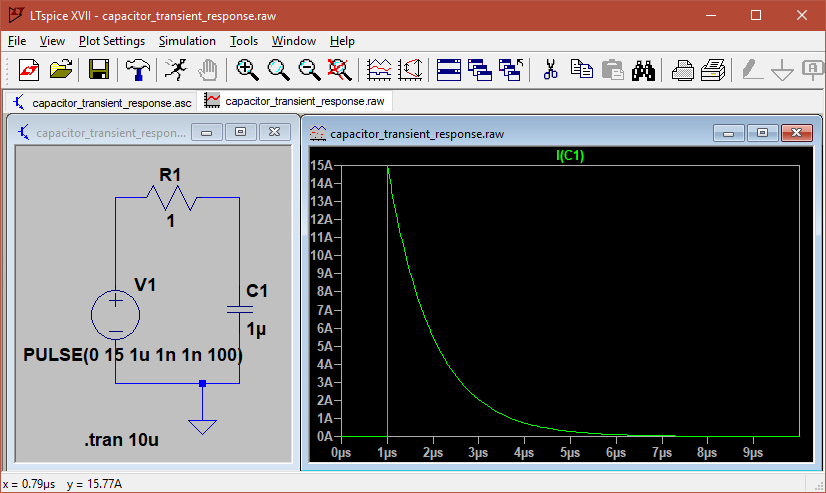
\includegraphics[width=\linewidth]{01-fig-ltspice.png}
	\caption{Graphical user interface of LTspice}
	\label{fig:ltspice-gui}
\end{figure}

\section{Use of Circuit Simulators Outside Industry}
The Berkeley SPICE programs were designed from the start to be used as an aid for integrated circuit designers. The same can be said about SPICE's successors that are used today. However, thanks to a significant increase in computational power, it is now possible to use circuit simulators in other contexts too. There is ongoing research on the use of evolutionary algorithms to evolve circuit parameters and even circuit topology. For example, in 2016, Rojec et al.\ successfully evolved a passive low-pass filter \cite{Rojec2016}. Also, computers and other interactive equipment are often used for educational purposes in schools, so a circuit simulator can be used as part of an educational program intended for high school or university students.

We have in mind creating such applications, and their development would be greatly simplified if there was a suitable circuit simulation library. We would essentially like the simulator to allow what we will call a \textit{live simulation}. For example, in a potential educational program, we would like to allow the user (a student) to e.g.\ flip switches or manipulate parameters of individual devices (e.g.\ resistances on the resistors), and hence provide an interactive experience. Also, circuit evolution applications could also make use of the possibility to simply manipulate circuit parameters. The first step of development of these applications would be finding and preparing such a simulation library.

Since such applications would be used primarily for academic or educational purposes, it is desired that these programs be easy to develop, maintain, and -- in the case of educational applications -- support multiple platforms. For these reasons it is probable that these applications would not be developed in some low level language like C++, but rather a higher level language. One such language, C\#, is part of the .NET developer platform, which is widely used in desktop application development. In recent years, .NET has expanded to other platforms as well and would be therefore our choice for the development of said applications.

As we have written earlier, SPICE programs and their descendants were designed mainly to be an aid for electrical engineers. As a consequence, they can only perform off-line simulation, where the simulated period needs to be set explicitly before the simulation starts. During our research we did not find any simulator which would allow the simulation to be continued where it left off.\footnote{For simple circuits, this can be achieved by setting the initial conditions of the circuit devices to be equal to the state of the circuit at the end of previous simulation, and recomputing the parameters for input sources (like phase offset and pulse delay). However, it is impossible to get or let alone set state of a device inside a subcircuit (the X device).} Furthermore, most simulators do not offer a binary API for other programs to use, which means that the communication with the simulator needs to be done through the SPICE netlist files. One simulator which stands out is ngspice \cite{ngspice}, which exposes a set of functions that allow manipulation of the simulator from an external program. The ngspice API does not require the input file to be written on disk, but we are still required to convert a simulated circuit into a netlist description, which is then passed to ngspice using a \texttt{char**} pointer.\footnote{For more details, see section 19.3 (Shared ngspice API) in ngspice user manual \cite{ngspice-manual}.}

Existing simulator programs therefore are not suitable for our purpose, we should search among the existing simulator libraries. At the time of assignment of this thesis, there was no implementation of a circuit simulation library for the .NET Framework.\footnote{At the time of writing, there is the SpiceSharp \cite{spicesharp} library, whose development started shortly after that of NextGen SPICE.} There are libraries for Python, for example PySpice \cite{pyspice} and PyOPUS \cite{pyopus} -- but these two libraries rely on standalone simulators (namely ngspice \cite{ngspice} and HSPICE \cite{hspice}) to do the simulation and therefore share the same limitations. There is also the JSpice \cite{jspice} library for Java, which implements it's own simulation engine, but just like other simulators requires the user to specify a simulation duration beforehand.

A possible solution to the problems of using present-date simulator programs or libraries is rewriting an existing circuit simulator in the .NET Framework and making necessary changes to the interface for our purpose. Berkley SPICE3 is still considered a reference simulator program, and since it is open source and freely available on the website of University of California, Berkeley \cite{spice3f5}, we will examine the possibility of rewriting it in .NET in the next subsection.

\subsubsection*{Rewriting SPICE3 for .NET, a Viable Option?}

SPICE3 was written in now non-standard K\&R C, because the development started years before the first ANSI norm was released in 1990. Due to the nature of the C language, many parts of the simulator are very fragile and hard to maintain from today's perspective. Consider the snippet in figure~\ref{fig:vccs_snippet} taken from the last SPICE3 release (version 3f.5 from 1993). It contains a function which loads instances of voltage controlled current source devices to a circuit equation matrix. This function is just one example from the set of functions that must exist for each device in the SPICE3 implementation. Other such functions include methods for model updating and data printing.

\begin{figure}[h]
	\begin{minted}[linenos, tabsize=4]{cpp}
/*ARGSUSED*/
int
VCCSload(inModel,ckt)
	GENmodel *inModel;
	CKTcircuit *ckt;
		/* actually load the current values into the 
		 * sparse matrix previously provided 
		 */
{
	register VCCSmodel *model = (VCCSmodel *)inModel;
	register VCCSinstance *here;
	
	/*  loop through all the source models */
	for( ; model != NULL; model = model->VCCSnextModel ) {
		
		/* loop through all the instances of the model */
		for (here = model->VCCSinstances; here != NULL ;
		here=here->VCCSnextInstance) {
			
			*(here->VCCSposContPosptr) += here->VCCScoeff ;
			*(here->VCCSposContNegptr) -= here->VCCScoeff ;
			*(here->VCCSnegContPosptr) -= here->VCCScoeff ;
			*(here->VCCSnegContNegptr) += here->VCCScoeff ;
		}
	}
	return(OK);
}
	\end{minted}
	\caption{Code snippet from \texttt{spice3f5/src/lib/dev/vccs/vccsload.c}}
	\label{fig:vccs_snippet}
\end{figure}

There are many points worth mentioning. In the declaration of the \texttt{VCCSload} function, the function parameters are specified by name only (line 3). The type of each parameter is then specified separately (lines 4--5). This is the main characteristic of K\&R C. In ANSI C, the equivalent declaration would be \texttt{VCCSload(GENmodel *inModel, CKTcircuit *ckt)}.

The next thing to notice is the pointer casting on line 10 -- the \texttt{inModel} parameter is cast to a pointer to the concrete type of the device that is being loaded. Practices like this are very common in C code due to the lack of higher-level language features like inheritance and polymorphism. Also, because no type checking occurs in C during pointer casting, it can be a source of hard-to-debug errors if the target object is of a different type.

Lines 10 and 11 also include the \texttt{register} keyword, which used to be a hint for the compiler to store the variable in a CPU register for faster access. This keyword is now deprecated, because modern compilers can do a better job at assigning variables to registers than a human programmer.

The last point worth noticing is the usage of pointers when accessing the equation matrix (lines 20 to 23). C\# does allow the usage of pointers in a so called \textit{unsafe code block}, but they affect the performance of the garbage collector, and should be used carefully.

Although it is possible to extend SPICE3 with new circuit devices by following instructions from Thomas Quarles, the author of SPICE3 \cite{Quarles:M89/45}, adding new analysis types requires modifying method tables for all existing devices and other crucial parts of the simulator, and thus is time consuming and error-prone.

The SPICE3 code also makes heavy use of \texttt{\#define} \texttt{\#ifdef} and other preprocessor directives which make the source code less readable. In combination with long functions and scarce source code documentation available (for an example, see file \texttt{spice3f5/src/lib/ckt/dctran.c}), rewriting the simulator is a very hard task requiring in-depth analysis and understanding of the simulator internals.

Overall, the programming style used in the SPICE3 implementation is very different from the style used in modern object oriented programming languages like C\#, and its code is not suitable for simple one-to-one translation from C to C\#.

\subsubsection*{Main thesis goal}
Because of the reasons listed so far in this chapter, computer programs which would as part of their functionality perform live simulation of electrical circuits would have to implement their own simulator engine. As the primary goal of this thesis, we would like to simplify the development of such applications by implementing such a circuit simulator from the ground up in the form of a portable .NET library. We will specify our requirements for the library in the next section.

\section{Reimplementation of SPICE for .NET}

Modern circuit simulators can do many types of circuit analyses and support many types of circuit devices. Because implementing a range of functionality comparable to these programs would be out of scope of this thesis, we have selected a reasonable subset to be implemented, which is described in the following subsection in greater detail. However we would like to be able to implement other features in the future without affecting the user's code. We would therefore have to design the library to be appropriately extensible.

\subsubsection*{Requirements on the Library}

We would like the library to be usable in broad contexts. Since .NET is now supported on many platforms, including Windows, Linux, and even mobile devices (Android, iOS and Windows Mobile), the library should be targeted to .NET Standard to make it maximally portable and usable on any .NET platform.

Our primary goal in the library will be supporting live simulation, as we described earlier. This essentially requires implementing the equivalent of \textit{transient analysis} of the SPICE simulator. However, the simulator should perform the individual timesteps on demand and allow making reasonable changes to the circuit devices like flipping switches, changing resistances, changing values of voltage and current sources.

Transient analysis requires so called \textit{large-signal} models of the simulated devices, which are also used by other types of SPICE-like analyses, like DC Sweep Analysis. DC Sweep analysis calculates the circuit states for a range of values for a certain circuit parameter (like the resistance of a resistor or the value of a voltage/current source). Because we already wish to support changing parameters between individual timesteps, our library will also support DC Sweep analysis.

We would like to design our library so that it could potentially support the same set of devices as the SPICE simulators. However, the implementation of all SPICE devices is quite complex and would be out of scope of this thesis. We have therefore decided to implement basic devices like ideal resistors, voltage or current sources, capacitors and inductors. Also, to demonstrate that even complex semiconductor devices can be implemented, we will implement diode and BJT transistor devices as well. These two devices are reasonably simple to implement and at the same time complex enough to demonstrate the capabilities of the simulator. Because SPICE is considered the reference circuit simulator implementation, we would implement these devices using the same mathematical models that are used in the SPICE simulators.

In the future, we would also like to add other types of circuit analyses -- such as AC frequency sweep analysis -- and new devices, and even allow users of our library to implement their own. The library should be therefore extensible without modifying the core library's source code. 

To provide academic researchers with a way to test newly developed models and computational techniques, the library should be widely configurable, and preferably open-source, to allow its users to contribute to the library's development.

Also, since there already exist vast libraries of spice circuits and subcircuits with macromodels described in the industry-standard SPICE netlist syntax, we would like to our library to support importing circuits from SPICE netlists. We will therefore provide a SPICE netlist parser as part of our library.

Since we have to recognize great portion of the SPICE netlist syntax in order to parse macromodel descriptions, with little additional work we could implement a parser to recognize control statements for requesting individual circuit analyses (like the \texttt{.OP} statement we saw in figure~\ref{fig:example_circuit}). This would allow us to create a console application similar to the original SPICE and therefore allow capabilities of the library to be used in a standalone fashion using the SPICE netlist syntax. Since .NET Standard cannot be used to develop console applications, we require that the console application requires the next smallest set of API: .NET Core. Figure~\ref{fig:deps} shows the expected relationship between the simulator, console application and other programs that would use the simulator -- parts in blue will be implemented as part of this thesis.

\begin{figure}[h]
	\centering
	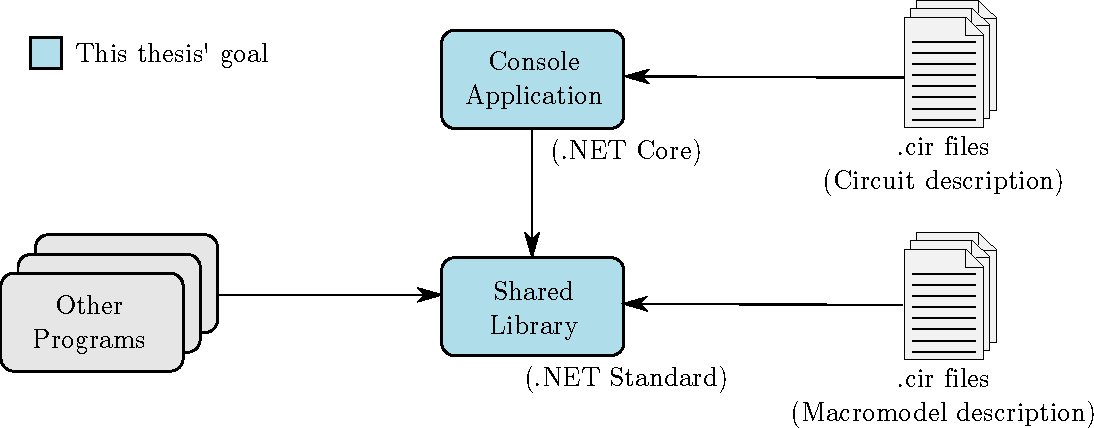
\includegraphics[width=0.8\linewidth]{deps-intro}
	\caption{Dependency diagram for NextGen SPICE and other programs}
	\label{fig:deps}
\end{figure}


\subsubsection*{Nonconvergence Due to Low Precision}
\label{chap:intro:dd}
Implementing any kind of simulation software means choosing an appropriate mathematical model for the given problem domain and, subsequently, a suitable representation of the problem in computer memory. Representing real numbers is an integral part of every physics simulation engine.

To achieve fast simulations, developers have to choose between representations having hardware support on the target platforms, which leaves them with IEEE 32-bit (\texttt{single}) and 64-bit (\texttt{double}) floating-point types. 

Most of the common circuit simulators use type \texttt{double} with approximately 15 decimal digits of precision. Due to the large dynamic range of the circuit variables, this leads to significant truncation errors when equation system coefficients differ in more than 15 orders of magnitude.

Coefficient differences of this magnitude may commonly occur when resistors with very small resistance values are used. Mike Robbins, one of the authors of the online circuit simulator CircuitLab, provides a simple example of such an ill-conditioned circuit in an article on their website \cite{circuitlab_dd}. This circuit along with the (partial) result plot from LTspice can be found in the upper part of figure~\ref{fig:ltspice-precision}. Notice the noise at the end of the simulated period emphasized by the red arrow. The lower part contains result of the same circuit in the CircuitLab simulator.\footnote{Keen reader might notice differences between the plot of CircuitLabs simulator results shown in this thesis and the one in the referenced article. These are due to the fact that CircuitLab uses slightly different model parameters for 1N4148 diode than LTspice. Plot shown in this thesis was obtained using the model parameters extracted from LTspice model library.}

\begin{figure}[h]
	\centering
	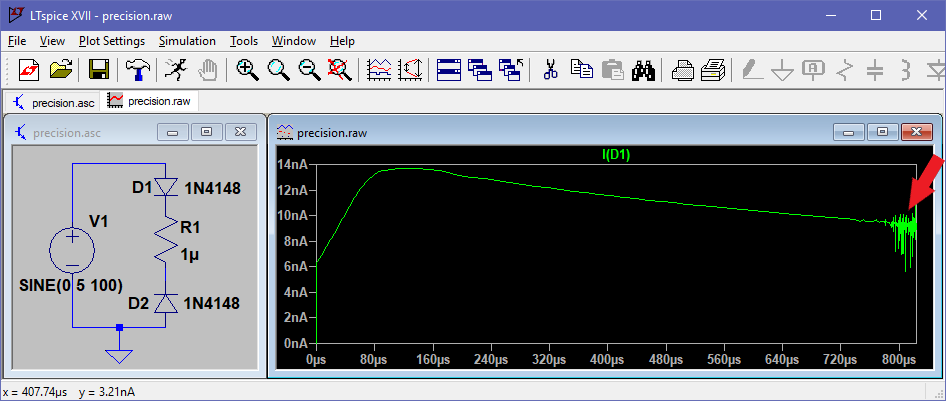
\includegraphics[width=0.8\textwidth]{01-fig-ltspice-precision}
	\caption*{LTspice}
	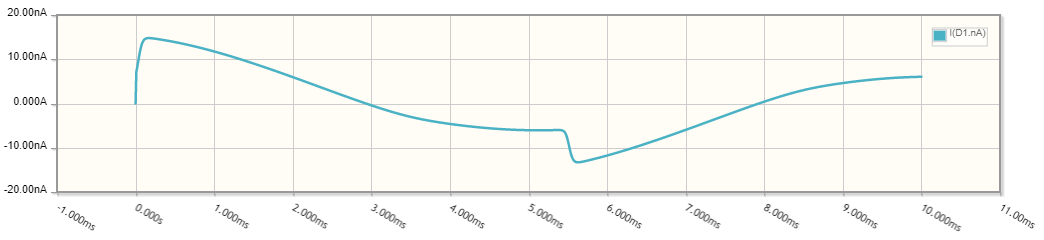
\includegraphics[width=0.8\textwidth]{01-fig-ltspice-precision2}
	\caption*{CircuitLab}
	\caption{Example ill-conditioned circuit, and example results form LTspice (top, incomplete), and CircuitLab (bottom), adapted from \cite{circuitlab_dd}}
	\label{fig:ltspice-precision}
\end{figure}

The noise in the plot on the figure is caused by the $1\mu\Omega$ resistor in the circuit. In the comment section under the article, Robbins writes that such small resistors are not physical, meaning that they do not correspond to physical resistor devices, but can be produced during automated macromodel construction. Use of this small resistor led to too-big differences between the equation coefficients, which in turn led to significant truncation errors and produced noise seen in the plot. This noise later leads to nonconvergence of the equation solution. Nonconvergence of the solution is a rather technical issue, and essentially means that the simulator cannot determine the state of the circuit after the next timestep.\footnote{In general, there are many reasons why solution might not converge, several possible techniques and simulator parameters used to overcome nonconvergence are explained in Ron Kielkowski's Inside SPICE \cite{inside_spice}.} In this case, the nonconvergence is caused by low precision of the representation of real numbers.

Such noise can be eliminated by using a more precise real number representation. One such option is using another type defined by the IEEE 754 standard, namely 80-bit or even 128-bit floating point number formats. However, neither of these is commonly available on today's hardware, let alone in the .NET runtime. If we would decide to use one of these two formats, every operation on such numbers would have to be emulated in software, which would greatly slow down the simulator.

Another option would be using the .NET type \texttt{decimal} which is a 128-bit representation of floating point numbers different from the IEEE 128-bit format. Its format is not directly supported on currently used processors, and therefore all operations are implemented in software by bit manipulations. Also, this type is intended mainly for handling currency and has an approximate range of only $-7.9 \cdot 10^{28}$ to $7.9 \cdot 10^{28}$,  which is too-narrow for circuit simulation.

Instead, in the article mentioned above, Mike Robbins proposes using the double-double technique. This technique represents a single value as a unevaluated sum of two \texttt{double} floating point values, each of which has its own significand and exponent. This principle is illustrated in figure~\ref{fig:dd_pi} where number $\pi$ is represented as a sum of two doubles.\footnote{One thing worth noting is that an implementation of the double-double format needs to decompose values based on the the binary representation of the real numbers. The QD library by Hida et al.\ \cite{qd-lib} uses values 3.141592653589793116e+00 and 1.224646799147353207e-16 in the source code, possibly to compensate errors from truncating periodic binary representation of the mantissa.}

\begin{figure}[h]
	\centering	
$\underbrace{3.141592653589793}_{ }\underbrace{238462643383279}$ 

$3.141592653589793 \cdot 10^{0} + 2.38462643383279 \cdot 10^{-16}$

	\caption{Decomposition of $\pi{}$ using double-double technique}
	\label{fig:dd_pi}
\end{figure}

Contrary to the options mentioned above, operations on the double-double format are implemented using standard operations on the \texttt{double} format, which are supported in today's hardware. This means that much higher speeds can be achieved. Hida et al.\ created a C++ library, that implements both double-double arithmetic, and it's slightly more complicated version -- quad-double arithmetic. More details about the algorithms used can be found in their published paper \cite{Hida2007}. 

Using these enhanced precision types is attractive, because they can solve some convergence issues during simulation, and we would therefore like to use them in our library. However, use of these precision types could lead to significant slowdown of the simulation, because multiple primitive operations on \texttt{double}s are done for each operation on the double-double and quad-double types. This could unnecessarily slow down simulations of circuits which do not require the precision provided by these types. We would therefore like to make these enhanced precision types optional, and otherwise use the standard \texttt{double} precision type. Because our implementation will allow using any of the \texttt{double}, double-double and quad-double types, we would like to compare the simulator performance -- i.e.\ speed and accuracy -- when using each of these types to get the basic idea when use of these types is appropriate.

\section{Goals}
\label{chap:intro:goals}

\begin{enumerate}
	\item Implement a SPICE-like simulation library	
	\begin{enumerate}
		\item Target .NET Standard for maximum portability
		\item \label{goal:transient} Support performing time-domain simulation of the circuit, and allow changing parameters of circuit devices between individual timesteps.
		
		\item \label{goal:devices} Support the following set of devices
		\begin{enumerate}
			\item Ideal resistor
			\item Ideal voltage source
			\item Ideal current source
			\item Ideal inductor
			\item Ideal capacitor
			\item SPICE diode
			\item SPICE BJT transistor
		\end{enumerate}
	
		\item \label{goal:extension} Allow new types of circuit analyses and circuit devices to be added to the simulator without modifying the library's source code.
	
		\item \label{goal:parser} Implement a SPICE netlist parser to allow importing circuits and macromodels from standard SPICE netlist files.

		\item \label{goal:dd} Allow users of the library to choose between double, double-double, and quad-double precision types and compare the library's performance with respect to speed and accuracy for each listed precision type.
	\end{enumerate}

	\item \label{goal:app} Use the simulation library to implement a SPICE-like console application for .NET Core, which would accept the implemented subset of SPICE netlist syntax.
\end{enumerate}

\chapter{The SPICE Netlist Syntax}
\label{chap:spicecode}

This chapter presents the netlist syntax, which we plan to support in the NextGen SPICE library for importing circuits and in the standalone console application. The syntax presented here is a subset of that supported by SPICE3, and can be further restricted to that of SPICE2.

\section{General Syntax}
\label{chap:spicecode:general}
The SPICE netlist syntax is case insensitive. A netlist file consists of individual statements, which are separated by line breaks. If a statement is to span multiple lines, every subsequent line must be prefixed with a + symbol. The following code fragments are therefore equivalent. 

\begin{code}
V1 0 1
+ SIN 0 5V 10KHZ
\end{code}

\begin{code}
V1 0 1 SIN 0 5V 10KHZ
\end{code}

Statements themselves are made up of individual data fields, delimited by blank characters. The meaning of data fields depends on the actual statement and on the position inside the statement. Generally, a data field specifies either a name, or a numeric value, and is then called a name field or a number field, respectively.

\subsection{Number Fields}
\label{chap:spicecode:numfield}
If the statement expects a data field to represent a numeric value, then the (number) field should start with a digit. However, if a decimal number is specified, the leading zeros may be omitted (therefore, \texttt{.05} is a valid number field having the same value as \texttt{0.05}). It is also possible to specify the scale by either using suffixes like \texttt{E-9} or one of the scaling factors listed in the following table.

\begin{center}
\begin{tabular}{|l|l|}	
	\hline
	Factor & Scale \\
	\hline \hline
	T & $ 10^{12} $ \\ \hline
	G & $10^9$ \\ \hline
	MEG & $ 10^6 $ \\ \hline
	K & $ 10^3 $ \\ \hline
	M & $ 10^{-3} $ \\ \hline
	U & $ 10^{-6} $ \\ \hline
	N & $ 10^{-9} $ \\ \hline
	P & $ 10^{-12} $ \\ \hline
	F & $ 10^{-15} $ \\
	\hline
\end{tabular}
\end{center}

Any additional characters that follow the number and scale factor are ignored, so the fields \texttt{10000}, \texttt{10E+3V}, \texttt{10K}, \texttt{10KV}, \texttt{10KVOLTS} and \texttt{10KHz} all represent the same value. This is convenient, because the ignored part may be used to specify units and thus improve readability of the netlist file.

\subsection{Name Fields}

On the other hand, if a data field is to represent a name, an arbitrary string of alphanumeric characters can be used.

\subsection{Comments}
The input file can also contain comments, which are completely ignored by the parser. Comments begin with an asterisk * symbol, and end by a line break. Comments can be used to further improve readability of the netlist file.

\begin{code}
V1 0 in 5 		* a 5V voltage source between the ground and 'in' node
\end{code}

\section{Data Statements}
\label{chap:spicecode-devices}

Data statements are used to describe the actual circuit and can be further divided into \textit{device statements} and \textit{model statements}. Device statements specify individual circuit devices and their connections to circuit nodes and generally have the following form:

\begin{code}
<device name> <terminal connections> <device arguments>
\end{code}

The concrete SPICE device type is determined by the first letter of the device name, and from the device type, the number of terminal connections and arguments is derived. Like SPICE3, we will not pose any restrictions on the length of the device name.\footnote{in SPICE2, the length was limited to seven characters only}

After the name follows a list of nodes to which the device connects. Nodes are identified by arbitrary alphanumeric strings.\footnote{In SPICE2, nodes are identified by integers, one consequence of this is that \texttt{00} and \texttt{0} are equivalent in SPICE2, but not in SPICE3.} The ground node is identified as \texttt{0}. After the terminal connections follows a device dependent argument list.

Model statements are used to specify parameters for more complex semiconductor devices, so that multiple devices can have the same parameters without their extensive repetition throughout the netlist file. A model statement has the following structure:

\begin{code}
.MODEL <model name> <model type> (<model parameter list>) 
\end{code}

Each device can accept only model types corresponding to that particular device type. Each model type has a set of parameters, which are set in the model parameter list, each having its default value. When defining a new model, only non-default values need to be specified by a list of key value pairs in the form \texttt{<name>=<value>}. The model name is then supplied as an argument to semiconductor devices such as a diode. 

The following sections describe the formats of several SPICE device statements. Values beginning with N are for node connections, values enclosed in square brackets are optional. Also, when applicable, the available model types and names of their parameters are listed.

\subsection{Resistor}

\begin{circuitdev}
	(0,0) node[label=N+]{} to[R, *-*] (2,0) node[label=N-]{}
\end{circuitdev}

\begin{code}
R<name> N+ N- <resistance>
\end{code}

A simple ideal resistor device. The order of N+ and N- nodes has no effect on the circuit behavior.

Examples: 

\begin{code}
R1 1 2 5OHM
R2 2 3 1K
\end{code}

\subsection{Capacitor}

\begin{circuitdev}
	(0,0) node[label=N+]{} to[C, *-*] (2,0) node[label=N-]{}
\end{circuitdev}

\begin{code}
C<name> N+ N- <capacitance> [IC=<initial voltage>]
\end{code}

An ideal capacitor device, an initial voltage can be specified to set a specific condition at the beginning of the simulation. If an initial condition is not present, the capacitor is modeled as an open circuit in the first DC operating point calculation.

Examples: 

\begin{code}
C1 1 2 1F
C2 2 3 1N IC=1M
\end{code}

\subsection{Inductor}

\begin{circuitdev}
	(0,0) node[label=N+]{} to[L, *-*] (2,0) node[label=N-]{}
\end{circuitdev}

\begin{code}
L<name> N+ N- <capacitance> [IC=<initial current>]
\end{code}

An ideal inductor device, an initial current can be specified to set a specific condition at the beginning of the simulation. If an initial condition is not present, the inductor is modeled as an ideal short circuit in the first DC operating point calculation.

Examples: 

\begin{code}
L1 1 2 1F
L2 2 3 1N IC=1M
\end{code}

\subsection{Input sources}
\label{chap:spicecode-input-sources}

\begin{circuitdev}
	(0,0) node[label=N+]{} to[V, *-*] (2,0) node[label=N-]{}
	(4,0) node[label=N+]{} to[I, *-*] (6,0) node[label=N-]{}
\end{circuitdev}

\begin{code}
V<name> N+ N- <source function>
I<name> N+ N- <source function>
\end{code}

NextGen SPICE supports complex specification of input source behaviors. Possible source functions are listed below.

\subsubsection{DC Source}
\begin{code}
[DC] <voltage>
\end{code}

A source that has a constant value, the \texttt{DC} identifier can be omitted.

Examples:

\begin{code}
V1 1 0 5V
I2 1 2 DC 10KV
\end{code}

\subsubsection{Sinusoidal Source}

\begin{code}
SIN <vo> <va> <freq> [<td> [<th> [<ph>]]]
\end{code}

\begin{center}
\begin{tabular}{|l|l|}
	\hline
Parameter & Meaning \\ \hline \hline
\texttt{<vo>} & Value offset \\ \hline
\texttt{<va>} & Value amplitude \\ \hline
\texttt{<fr>} & Waveform frequency \\ \hline
\texttt{<td>} & Delay time \\ \hline
\texttt{<th>} & Damping factor \\ \hline
\texttt{<phase>} & Phase offset \\ \hline
\end{tabular}
\end{center}

A sinusoidal source with amplitude damping. The value of the source function is given by

\[f(t) = \begin{cases}

\texttt{<vo> } & \text{if } t < \texttt{<td>} \\
\texttt{<vo>} + \texttt{<va>} \begin{aligned}
&\cdot e^{- (t - \texttt{<td>}) \cdot \texttt{<th>}}\\
&\cdot \sin{(2 \pi \cdot  (\texttt{<fr>} \cdot (t - \texttt{<td>}) + \texttt{<ph>}))}
\end{aligned}  & \text{if } t \ge \texttt{<td>}
\end{cases}\] 


Example:

\begin{code}
V1 1 0 SIN 1 5 2KHZ 1MS 0.5K
\end{code}

\begin{center}
	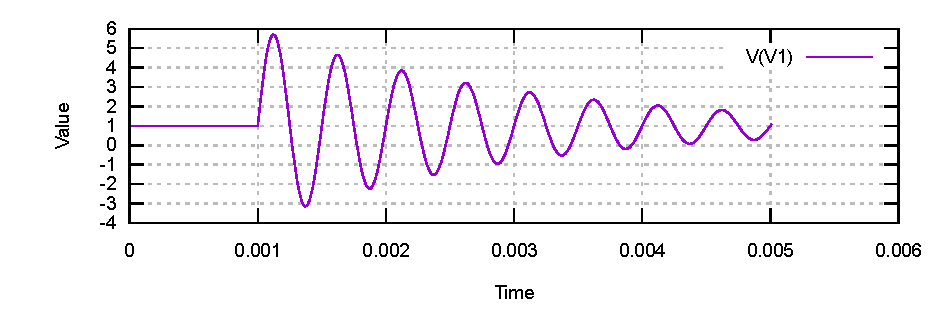
\includegraphics[width=0.85\linewidth]{source-sin}
\end{center}

\pagebreak
\subsubsection{Exponential Source}

\begin{code}
EXP <v1> <v2> [<td1> <tau1> [<td2> <tau2>]]
\end{code}

\begin{center}
	\begin{tabular}{|l|l|}
		\hline
		Parameter & Meaning \\ \hline \hline
		\texttt{<v1>} & Initial value \\ \hline
		\texttt{<v2>} & Pulse value \\ \hline
		\texttt{<td1>} & Delay before first e.g.\ \\ \hline
		\texttt{<tau1>} & First e.g.\ time constant \\ \hline
		\texttt{<td2>} & Delay before second e.g.\ \\ \hline
		\texttt{<tau2>} & Second e.g.\ time constant \\ \hline
	\end{tabular}
\end{center}

A pulsing source with exponential rising and falling edges. Values of the source are given by:

\[
f(t) = \begin{cases}
\texttt{<v1>} & \text{if } t < \texttt{<td1>} \\\\
\texttt{<v1>} + \left( \texttt{<v1>} - \texttt{<v2>} \left[1-e^{\frac{-(t-\texttt{<td1>})}{\texttt{<tau1>}}}\right] \right)& \text{if } \texttt{<td1>} \ge t > \texttt{<td2>} \\\\
\texttt{<v1>} \begin{aligned}
&+ \left( \texttt{<v1>} - \texttt{<v2>} \left[1-e^{\frac{-(t-\texttt{<td1>})}{\texttt{<tau1>}}}\right] \right) \\
&+ \left( \texttt{<v2>} - \texttt{<v1>} \left[1-e^{\frac{-(t-\texttt{<td2>})}{\texttt{<tau2>}}}\right] \right)
\end{aligned}& \text{if } t \ge \texttt{<td2>} \\
\end{cases}
\]

Example:

\begin{code}
V1 1 0 EXP 1 5 1MS 0.5M 4MS 0.1M 
\end{code}

\begin{center}
	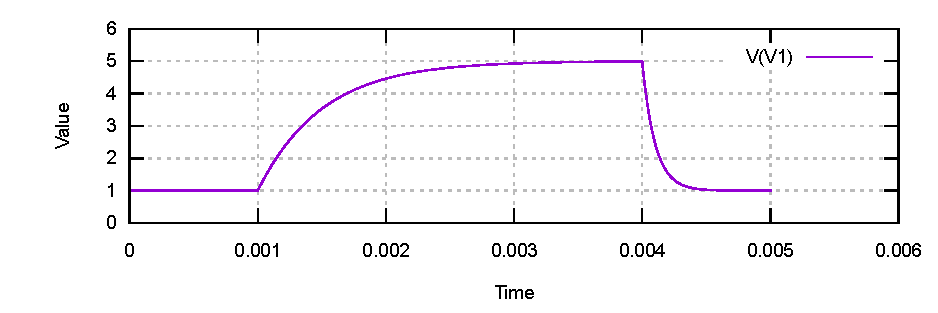
\includegraphics[width=0.85\linewidth]{source-exp}
\end{center}

\subsubsection{Pulse Source}

\begin{code}
PULSE <v1> <v2> <td> <tr> <tf> <ton> <period>
\end{code}

\begin{center}
	\begin{tabular}{|l|l|}
		\hline
		Parameter & Meaning \\ \hline \hline
		\texttt{<v1>} & Initial value \\ \hline
		\texttt{<v2>} & Pulse value \\ \hline
		\texttt{<td>} & Delay before rising e.g.\ of the pulse \\ \hline
		\texttt{<tr>} & Time of the rising e.g.\ of the pulse\\ \hline
		\texttt{<tf>} & Time of the falling e.g.\ of the pulse \\ \hline
		\texttt{<ton>} & Duration of the pulse \\ \hline
		\texttt{<period>} & Period of the source \\ \hline
	\end{tabular}
\end{center}

A source that sends individual pulses.

Example:

\begin{code}
V1 1 0 PULSE 1 5 1MS 0.5MS 1.5MS 1MS 5MS
\end{code}

\begin{center}
	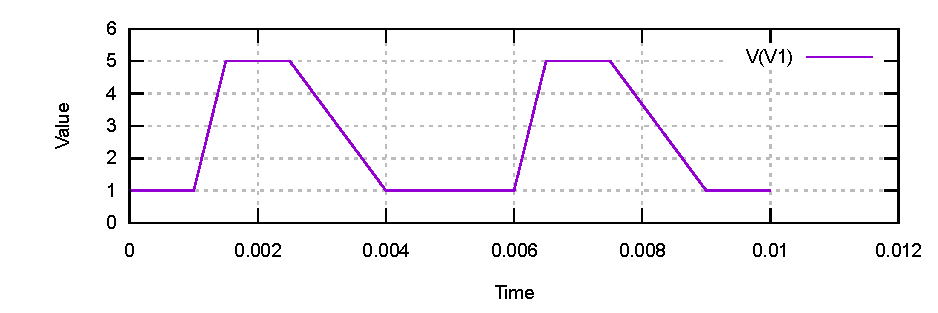
\includegraphics[width=0.85\linewidth]{source-pulse}
\end{center}

\subsubsection{Piecewise Linear Source}

\begin{code}
PWL <t1> <v1> [<t2> <v2> [<t3> <v3> [...]]]
\end{code}

An arbitrary piece-wise linear source. The argument list consists of pairs of timepoints and source values. The intermediate values are determined using linear interpolation.

Example:
\begin{code}
V1 1 0 PWL 0MS 1 1MS 2 3MS -1 3.1MS 0 5MS 1
\end{code}

\begin{center}
	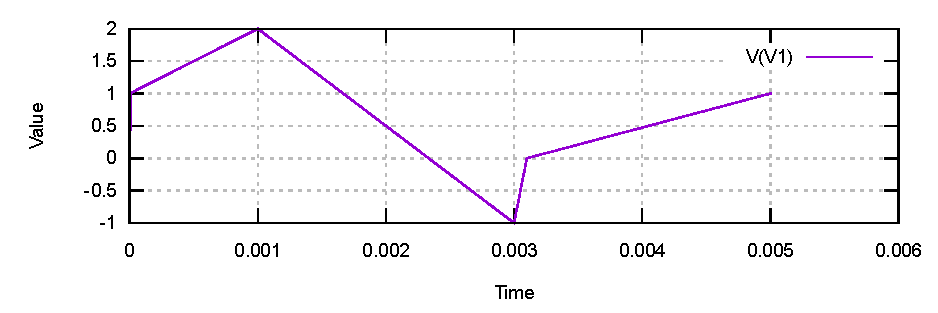
\includegraphics[width=0.85\linewidth]{source-pwl}
\end{center}

\subsubsection{AM Source}
\begin{code}
AM <amp> <dc> <fm> <fc> [<td> [<ph>]]
\end{code}

\begin{center}
	\begin{tabular}{|l|l|}
		\hline
		Parameter & Meaning \\ \hline \hline
		\texttt{<amp>} & Peak amplitude of the unmodulated signal. \\ \hline
		\texttt{<dc>} & DC offset \\ \hline
		\texttt{<fm>} & Modulation frequency \\ \hline
		\texttt{<fc>} & Carrier frequency \\ \hline
		\texttt{<td>} & Delay before the signal \\ \hline
		\texttt{<ph>} & Phase offset \\ \hline
	\end{tabular}
\end{center}

% arbitrary page break to better accmodate the pictures
\pagebreak
A source with an amplitude modulated signal. The value at any given timepoint is given by

\[
f(t) = \texttt{<amp>} \begin{aligned}
&\cdot \left( \texttt{<dc>}  + \sin{
	\left(
	2\pi \cdot \texttt{<fm>} \cdot  \left(t - \texttt{<td>}\right)
	\right)} + \texttt{<ph>} \right) 
\\
&\cdot \sin{
	\left(
	2\pi \cdot \texttt{<fc>} \cdot  \left(t - \texttt{<td>} \right) + \texttt{<ph>}
	\right)}.
\end{aligned} 
\]

Example:

\begin{code}
V1 1 0 AM 5 2 0.5KHZ 4KHZ 2MS
\end{code}

\begin{center}
	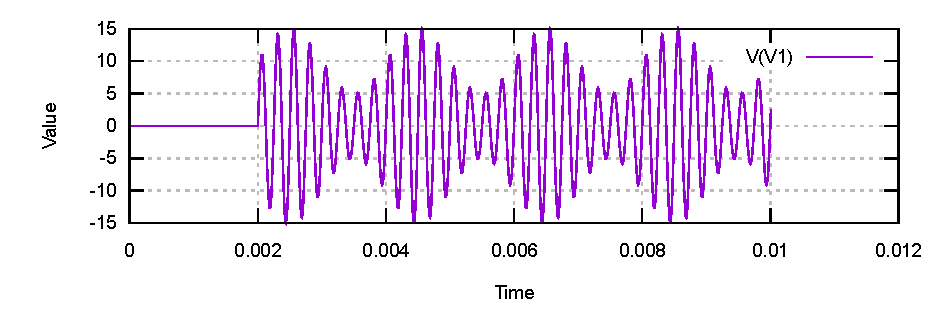
\includegraphics[width=0.85\linewidth]{source-am}
\end{center}

\subsubsection*{SFFM Source}
\begin{code}
SFFM <dc> <amp> <fc> <m> <fm>
\end{code}

\begin{center}
	\begin{tabular}{|l|l|}
		\hline
		Parameter & Meaning \\ \hline \hline
		\texttt{<dc>} & DC offset of the signal \\ \hline
		\texttt{<amp>} & Amplitude of the carrier. \\ \hline
		\texttt{<fc>} & Carrier frequency \\ \hline
		\texttt{<m>} & Modulation index \\ \hline
		\texttt{<fm>} & Modulation frequency \\ \hline
	\end{tabular}
\end{center}

A source with a frequency modulated signal. The value at any given timepoint is given by

\[
f(t) = \texttt{<dc>} + \texttt{<amp>} \cdot \sin{
	\left(
	2\pi \cdot \texttt{<fc>} \cdot  \left(t - \texttt{<td>}\right) + m \cdot \sin{
		\left(
		2\pi \cdot \texttt{<fm>} \cdot  \left(t - \texttt{<td>}\right)
		\right)}
	\right)}.
\]

Example:

\begin{code}
V1 1 0 SFFM 2 1 1KHZ 3 0.2KHZ 
\end{code}

\begin{center}
	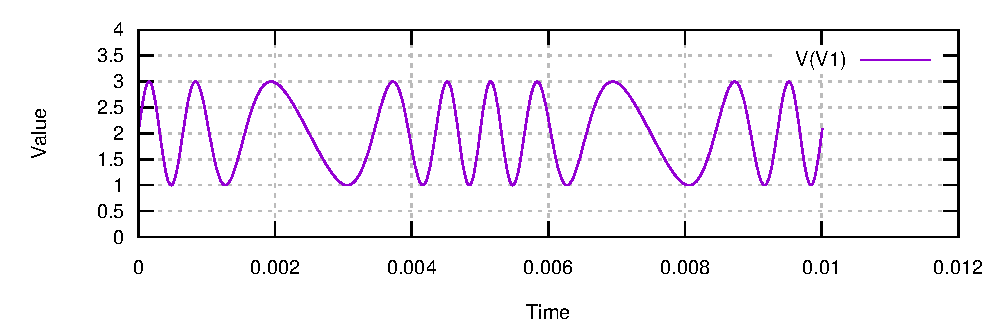
\includegraphics[width=0.85\linewidth]{source-sffm}
\end{center}


\subsection{Controlled Sources}

SPICE supports linear dependent sources, both current and voltage controlled. In the case of voltage controlled sources, an additional pair of terminals is specified, and the value of the source is linearly dependent on the voltage between those control terminals. In case of current controlled sources, the name of a voltage source is supplied and the value of the source depends linearly on the current flowing through said device.\footnote{The reason that only voltage source can be used is that the current flowing through the voltage source is directly accessible through a circuit variable in the equation system. Also, because earlier versions of SPICE could output only currents flowing through voltage sources, it became a standard practice to use 0V voltage sources as amperemeters.} The coefficient of linear dependence, called the \textit{gain} is supplied as the last parameter.

\subsubsection{Voltage Controlled Voltage Source}
\begin{circuitdev}
	(0,0) node[circ,label=NC+]{} 
	-- (1,0)
	-- (1,-2)
	-- (0,-2) node[circ,label=NC-]{}
	
	(3,0) node[circ,label=N+]{}
	-- (2,0)
	to[V] (2, -2)
	-- (3,-2) node[circ,label=N-]{}
\end{circuitdev}
\begin{code}
E<name> N+ N- NC+ NC- <gain>
\end{code}



Example: 

\begin{code}
E1 1 2 3 4 100
\end{code}


\subsubsection{Voltage Controlled Current Source}
\begin{circuitdev}
	(0,0) node[circ,label=NC+]{} 
	-- (1,0)
	-- (1,-2)
	-- (0,-2) node[circ,label=NC-]{}
	
	(3,0) node[circ,label=N+]{}
	-- (2,0)
	to[I] (2, -2)
	-- (3,-2) node[circ,label=N-]{}
\end{circuitdev}
\begin{code}
G<name> N+ N- NC+ NC- <gain>
\end{code}

Example: 

\begin{code}
G1 1 2 3 4 100
\end{code}


\subsubsection{Current Controlled Voltage Source}
\begin{circuitdev}
	(0,0) 
	-- (1,0)
	to[V,a=vsource] (1,-2)
	-- (0,-2)
	
	(4,0) node[circ,label=N+]{}
	-- (3,0)
	to[cV] (3, -2)
	-- (4,-2) node[circ,label=N-]{}
\end{circuitdev}
\begin{code}
H<name> N+ N- <vsource> <gain>
\end{code}

Example: 

\begin{code}
VMETER 1 2 0
H1 2 3 VMETER
\end{code}

\subsubsection{Current Controlled Current Source}
\begin{circuitdev}
	(0,0) 
	-- (1,0)
	to[V,a=vsource] (1,-2)
	-- (0,-2)
	
	(4,0) node[circ,label=N+]{}
	-- (3,0)
	to[cI] (3, -2)
	-- (4,-2) node[circ,label=N-]{}
\end{circuitdev}
\begin{code}
F<name> N+ N- <vsource> <gain>
\end{code}

Example: 

\begin{code}
VMETER 1 2 0
F1 2 3 VMETER
\end{code}

\subsection{Diode}
\begin{circuitdev}
	(0,0) node[label=N+]{} to[D, *-*] (2,0) node[label=N-]{}
\end{circuitdev}

\begin{code}
D<name> N+ N- <model name>
\end{code}

A semiconductor diode device. The physical parameters of a diode are set using a \texttt{.MODEL} statement with the \texttt{D} model type. The following table lists supported model parameters for the diode model. The parameters in gray are parsed, but do not affect the simulation in the current implementation.

\begin{center}
	\begin{tabu}{|l|l|r l|}
		\hline
		Parameter name & Description & \multicolumn{2}{l|}{Default value} \\ 
		\hline \hline
		IS & Saturation current & $ 1 \cdot 10^{-14}$& A  \\ \hline	
		RS & Ohmic resistance & $ 0 $& \\ \hline		
		N & Emission coefficient & $ 1 $& \\ \hline	
		TT & Transit-time current & $ 0$& s \\ \hline	
		CJO & Zero-bias junction capacitance & $ 0$& F \\ \hline	
		VJ & Junction potential & $ 1$& V \\ \hline	
		M & Grading coefficient & $ 0.5 $& \\ \hline	
		\rowfont{\color{lightgray}}	EG & Activation ene.g.\ & $ 1.11$& eV\\ \hline	
		\rowfont{\color{lightgray}}	XTI & Saturation-current temperature exponent & $ 3 $& \\ \hline	
		\rowfont{\color{lightgray}}	KF & Flicker noise coefficient & $ 0 $& \\ \hline	
		\rowfont{\color{lightgray}}	AF & Flicker noise exponent & $ 1 $& \\ \hline	
		\rowfont{\color{lightgray}}	FC & \makecell[l]{Coefficient for forward-bias \\
			 depletion capacitance formula} & $ 0.5 $&\\ \hline	
		BV & Reverse breakdown voltage & $ \infty{}$& V \\ \hline	
		\rowfont{\color{lightgray}}	IBV & Current at breakdown voltage & $ 1 \cdot 10^{-3}$& A \\ \hline	
		TNOM & Parameter measurement temperature & $ 27$& °C \\ \hline	
	\end{tabu}
\end{center}

Example:
\begin{code}
D1 1 2 1N4148
.MODEL 1N4148 D(IS=2.52N RS=.568 N=1.752 CJO=4P M=.4 TT=20N VJ=20 BV=75)
\end{code}

\subsection{BJT Transistor}
\begin{circuitdev}
(0,0) node[npn](npn1) {}
(npn1.base) node[circ, label=180:NB] {}
(npn1.collector) node[circ, label=NC] {}
(npn1.emitter) node[circ, label=270:NE] {}

(4,0) node[pnp,yscale=-1](pnp1) {}
(pnp1.base) node[circ, label=180:NB] {}
(pnp1.collector) node[circ, label=NC] {}
(pnp1.emitter) node[circ, label=270:NE] {};
\end{circuitdev}

\begin{code}
Q<name> NC NB NE <model name>
\end{code}

A semiconductor BJT transistor device. The physical parameters of a BJT are set using a \texttt{.MODEL} statement, as well as the polarity of the transistor. There are two model types for a BJT transistor: \texttt{NPN} and \texttt{PNP}. Both model types accept the same parameters, which are listed in the following table. The parameters in gray are parsed, but do not affect the simulation in the current implementation.

\begin{center}
	\begin{longtable}{|l|l|r l|}
		\hline
		\makecell[l]{Parameter \\ name} & Description & \multicolumn{2}{l|}{Default value} \\ 
		\hline \hline
		IS 	&	Transport saturation current	&	1.0e16 &	A 	 \\ \hline
BF 	&	Ideal maximum forward beta	&	100 &	 	 \\ \hline
NF 	&	Forward current emission coefficient	&	1.0 	   &	 	 \\ \hline
VAF 	&	Forward Early voltage	&	$ \infty{}$    &	V 	 \\ \hline
IKF 	&	Corner for forward beta high current roll-off	&	$ \infty{}$    &	A 	 \\ \hline
ISE 	&	B-E leakage saturation current	&	0 	&   	A 	 \\ \hline
NE 	&	B-E leakage emission coefficient	&	1.5 	&   	 	 \\ \hline
BR 	&	Ideal maximum reverse beta 	&	1 	&   	 	 \\ \hline
NR 	&	Reverse current emission coefficient	&	1 	&   	 	 \\ \hline
VAR 	&	Reverse Early voltage	&	$ \infty{}$    &	V 	 \\ \hline
IKR 	&	Corner for reverse beta high current roll-off	&	$ \infty{}$    &	A 	 \\ \hline
ISC 	&	Leakage saturation current	&	0 	&   	A 	 \\ \hline
NC 	&	Leakage emission coefficient	&	2 	&   	 	 \\ \hline
	RB 	&		Zero bias base resistance	&		0 	&	   	 	 \\ \hline
\color{lightgray}	IRB 	&	\color{lightgray}	\makecell[l]{Current where base resistance \\ falls halfway to its min value}	&	\color{lightgray}	$ \infty{}$ &	\color{lightgray}	A 	 \\ \hline
\color{lightgray}	RBM 	&	\color{lightgray}	Minimum base resistance at high currents	&	\color{lightgray}	RB  &	\color{lightgray}	 	 \\ \hline
RE 	&		Emitter resistance	&		0 	&	   	 	 \\ \hline
RC 	&		Collector resistance 	&		0 	&	   	 	 \\ \hline
CJE 	&		B-E zero-bias depletion capacitance	&		0 	&	   	F 	 \\ \hline
VJE 	&		B-E built-in potential	&		0.75    &		V 	 \\ \hline
MJE 	&		B-E junction exponential factor 	&		0.33    &		 	 \\ \hline
TF 	&		Ideal forward transit time 	&		0 	&	   	s 	 \\ \hline
\color{lightgray}	XTF	&	\color{lightgray}	Coefficient for bias dependence of TF 	&	\color{lightgray}	0 	&	\color{lightgray}   	 	 \\ \hline
\color{lightgray}	VTF 	&	\color{lightgray}	Voltage describing VBC dependence of TF 	&	\color{lightgray}	$ \infty{}$    &	\color{lightgray}	V 	 \\ \hline
\color{lightgray}	ITF 	&	\color{lightgray}	High-current parameter  for effect on TF 	&	\color{lightgray}	0 	&	\color{lightgray}   	A 	 \\ \hline
\color{lightgray}	PTF 	&	\color{lightgray}	Excess phase at freq=1.0/(TF*2PI) Hz 	&	\color{lightgray}	0 	&	\color{lightgray}   	deg 	 \\ \hline
CJC 	&		B-C zero-bias depletion capacitance 	&		0 	&	   	F 	 \\ \hline
VJC 	&		B-C built-in potential 	&		0.75    &		V 	 \\ \hline
MJC 	&		B-C junction exponential factor 	&		0.33    &		 	 \\ \hline
\color{lightgray}	XCJC 	&	\color{lightgray}	\makecell[l]{Fraction of B-C depletion capacitance \\ connected to internal base node} 	&	\color{lightgray}	1 	&	\color{lightgray}   	 	 \\ \hline
TR 	&		Ideal reverse transit time 	&		0 	&	   	s 	 \\ \hline
CJS 	&		Zero-bias collector-substrate capacitance 	&		0 	&	   	F 	 \\ \hline
VJS 	&		Substrate junction built-in potential 	&		0.75    &		V 	 \\ \hline
MJS 	&		Substrate junction exponential factor 	&		0 	&	   	 	 \\ \hline
\color{lightgray}	XTB 	&	\color{lightgray}	Forward and reverse beta  temperature exponent 	&	\color{lightgray}	0 	&	\color{lightgray}   	 	 \\ \hline
\color{lightgray}	EG	&	\color{lightgray}	Ene.g.\ gap for temperature  effect on IS 	&	\color{lightgray}	1.11    &	\color{lightgray}	eV 	 \\ \hline
\color{lightgray}	XTI	&	\color{lightgray}	Temperature exponent for effect on IS 	&	\color{lightgray}	3 	&	\color{lightgray}   	 	 \\ \hline
\color{lightgray}	KF 	&	\color{lightgray}	Flicker-noise coefficient 	&	\color{lightgray}	0 	&	\color{lightgray}   	 	 \\ \hline
\color{lightgray}	AF 	&	\color{lightgray}	Flicker-noise exponent 	&	\color{lightgray}	1 	&	\color{lightgray}   	 	 \\ \hline
FC 	&		\makecell[l]{Coefficient for forward-bias \\ depletion capacitance formula} 	&		0.5 	&	   	 	 \\ \hline

TNOM 	&	Parameter measurement temperature 	&	27  &	°C 	 \\ \hline


	\end{longtable}
\end{center}

Examples:

\begin{code}
Q1 1 2 3 QMOD1
.MODEL QMOD1 PNP(IS=1P)

Q2 4 5 6 QNL
.MODEL QNL NPN(BF=80 RB=100 TF=0.3NS TR=6NS CJE=3PF CJC=2PF VAF=50V)
\end{code}

\subsection{Subcircuits}
\label{chap:spicecode:subcircuits}
Subcircuits are a SPICE netlist term for device macromodels mentioned back in the introduction chapter. The following syntax is used.

\begin{code}
.SUBCKT <subcircuit name> <terminal nodes>
<subcircuit description>
.ENDS
\end{code}

The description of the subcircuit has to be enclosed between \texttt{.SUBCKT} and \texttt{.ENDS} statements. The \texttt{.SUBCKT} statement states the name of the subcircuit and lists the names of terminal nodes, which will then be used to connect the subcircuit to the outer circuit. There must be at lesat one terminal node and none of them can be 0 (the ground node).

The actual description of the subcircuit can contain only data statements -- device statements, \texttt{.MODEL} statements, and other \texttt{.SUBCKT} statements. Also, it is customary to place a comment line describing the meaning of the terminal nodes (like in figure~\ref{fig:example_subcircuit}).

Any names defined inside a subcircuit are strictly local to the subcircuit. Therefore, models and subcircuits defined inside the subcircuit cannot be used after the \texttt{.ENDS} statement.

A subcircuit can then be used as an individual device by the following syntax:

\begin{code}
X<name> <terminal nodes> <subcircuit name>
\end{code}

where \texttt{<subcircuit name>} is the name supplied in the corresponding \texttt{.SUBCKT} statement, and \texttt{<terminal nodes>} names the appropriate number of nodes to which the subcircuit should connect.

Example:
\begin{code}
.SUBCKT ACAMPLIFIER 2 1 3
R1 1 4 2K
R2 4 0 500
C1 2 4 10n
Q1 3 4 5 2N2222
Rc 1 3 2K
Re 5 0 1e3
.MODEL 2N2222 PNP(BF=50 IS=1E-13 VBF=50)
.ENDS

XOPAMP 1 2 3 ACAMPLIFIER
\end{code}

\subsection{Summary of the Device Statements}

\begin{center}
	\begin{tabular}{|l|l|}
		\hline
		Device & Syntax \\ 
		\hline \hline
		Resistor & \texttt{R<name> N+ N- <resistance>} \\ \hline
		Capacitor & \texttt{C<name> N+ N- <capacitance> [IC=<voltage>]} \\ \hline
		Inductor & \texttt{L<name> N+ N- <inductance> [IC=<current>]} \\ \hline
		Voltage source & \texttt{V<name> N+ N- <source function>} \\ \hline
		Current source & \texttt{I<name> N+ N- <source function>} \\ \hline
		\makecell[l]{Voltage controlled \\ voltage source} & \texttt{E<name> N+ N- NC+ NC- <gain>} \\ \hline
		\makecell[l]{Voltage controlled \\ current source} & \texttt{G<name> N+ N- NC+ NC- <gain>} \\ \hline
		\makecell[l]{Current controlled \\ voltage source} & \texttt{H<name> N+ N- <voltage source> <gain>} \\ \hline
		\makecell[l]{Current controlled \\ current source} & \texttt{F<name> N+ N- <voltage source> <gain>} \\ \hline
		Diode & \texttt{D<name> N+ N- <model name>} \\ \hline
		BJT transistor & \texttt{Q<name> NC NB NE <model name>} \\ \hline
	\end{tabular}
\end{center}

\newpage
\section{Control Statements}

Control statements are used for performing circuit simulations.

\subsection{.OP Statement}

\begin{code}
.OP
\end{code}

The \texttt{.OP} statement is used for requesting DC operating point analysis, which means calculating the values of node voltages and branch currents corresponding to a stable state of the circuit. This statement does not have any arguments.

\subsection{.TRAN Statement}

\begin{code}
.TRAN <timestep> <stop time> [<start time>]
\end{code}

This statement is used for requesting transient analysis --- time-domain simulation of the circuit --- for the specified duration with the given timestep. For each timepoint, an operating point is established, and time-dependent behavior of devices such as capacitor and inductor is modelled using numerical integration methods. If we are interested only in data after a certain timepoint, we can use the third optional parameter to instruct the simulator to not print simulation results until a certain timepoint.

\section{Output Statements}
\label{chap:spicecode-output}

Output statements can be used to select which data should be printed in the simulator's output. If no output statement is provided, NextGen SPICE will print all available data. Currently, the only supported statement is the \texttt{.PRINT} statement.

\begin{code}
.PRINT <analysis type> <list of requested data>
\end{code}

The analysis type is either \texttt{OP} or \texttt{TRAN}, indicating from which analysis type the data are requested. Following table summarizes the possible data specifiers.

\begin{center}
	\begin{tabular}{|l|l|}
		\hline
		Specifier & Description \\ \hline \hline
		\texttt{V(<node>)} & Voltage of the node \texttt{<node>} \\ \hline
		\texttt{V(<node1>,<node2>)} & Voltage between nodes \texttt{<node1>} and \texttt{<node2>} \\ \hline
		\texttt{V(<device>)} & Voltage across the \texttt{<device>} device\footnotemark  \\ \hline
		\texttt{I(<device>)} & Current flowing through the \texttt{<device>} device$^{\ref{footnote:spice_print}}$. \\ \hline
	\end{tabular}
\end{center}

\footnotetext{\label{footnote:spice_print}Only devices having exactly two terminals are allowed.}


\section{Netlist File Structure}
The structure of a netlist can be almost arbitrary, the only restrictions are that the first line, called the \textit{title line}, should contain a brief description of the netlist contents (and is not interpreted as a statement), and that the last statement is an \texttt{.END} statement. There are no restrictions on the relative order of statements in the netlist. For example, semiconductor device models can be used in device statements even before they are defined by their respective \texttt{.MODEL} statement. However, even though any order is possible, netlist files are commonly structured in the following manner:

\begin{itemize}
	\item Title
	\item Device statements
	\item \texttt{.MODEL} statements
	\item Control statements
	\item Output statements
	\item \texttt{.END} statement
\end{itemize}

\section{Circuit Topology Constraints}
\label{chap:spicecode:topology}

There are some restrictions on how circuit devices can be connected to nodes. These restrictions help ensure that the equation system rising from the simulated circuit always has a unique solution. The rules are the following:

\begin{itemize}
	\item The circuit may not contain cycles consisting of voltage defined devices (e.g.\ voltage sources and inductors)
	\item The circuit may not contain cutsets consisting of current defined devices (e.g.\ current sources and capacitors)
	\item In a circuit, there must exist a path from each node to the ground node
	\item In a subcircuit, there must exist a path between each pair of terminals that does not contain the ground node 
\end{itemize}

\chapter{Implementation Analysis}
\label{chap:analysis}

Just like other modern day circuit simulators, our library is also heavily influenced by the original Berkeley SPICE. We have decided to reflect this fact in the name our library and call it NextGen SPICE, and we will use this name in the remainder of this thesis.

This chapter analyses various possibilities of NextGen SPICE simulator implementation. The reader should be acquainted with the necessary theory of circuit simulation. Ron Kielkowski's Inside SPICE \cite{inside_spice} is an excellent source of details about the workings of SPICE-like simulators. The necessary mathematical theory is nicely summarized in the documentation of the QUCS simulator \cite{qucs}, which we will cite frequently in the next chapters. Another great source is the Ph.D. theses of Laurence W. Nagel (Author of SPICE2) \cite{Nagel:M520}. The last two sources are freely available and we include them on the attached CD for convenience.

\section{Initial Organisation of the library}

One of the goals of this thesis is the implementation of a configurable and extensible circuit simulation library. One of the requirements is that new types of circuit analyses as well as new circuit devices can be added without modification of the core library's source code (goal~\ref{goal:extension}). Before we start with the actual analysis, we will briefly describe how the original SPICE program operates. 

\subsection{Overview of SPICE Simulator Workflow}
\label{chap:analysis:spice-review}
The top level view on the SPICE simulator is summarized in figure~\ref{fig:spice-workflow}. The user specifies the circuit to be simulated inside a SPICE netlist file (1). This file is parsed by SPICE, which constructs an internal representation of the circuit (2) and validates the circuit topology according to the rules described in section~\ref{chap:spicecode:topology}. If the circuit is correctly formed, SPICE performs the simulations specified in the netlist file. This consists of mapping the devices into coefficients in an equation system characterizing the circuit (3). This equation system is then solved to obtain the result of the analysis, which is then stored in the circuit representation. The user-specified characteristics of the circuit devices are then printed to the output (4). 

\begin{figure}[h]
	\centering
	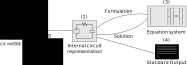
\includegraphics[width=0.8\linewidth]{spice-workflow}
	\caption{SPICE operation workflow.}
	\label{fig:spice-workflow}
\end{figure}


Because different analyses simulate different characteristics of circuit devices, most devices contribute to the equation system coefficients differently in each circuit analysis. To provide a concrete example, the following two paragraphs briefly describe two distinct kinds of circuit analyses: transient analysis (the implementation of which is part of this thesis), and AC frequency sweep analysis (which we would like to implement in future versions), and their specific way of simulating capacitors and inductors.

In transient analysis, the circuit's behavior is simulated over time. The first step of this analysis is calculating the initial DC bias of the circuit, which is the technical term for calculating the node voltages and currents flowing through the circuit branches. During this step, capacitors are modeled as ideal open circuits and inductors as ideal short circuits.\footnote{Consequence of modeling capacitor as open circuit and inductor as short circuit is that the simulation starts from a stable (quiescent) state of the circuit, SPICE simulators allow user to specify custom initial conditions: voltage across the capacitor and current flowing through the inductor, and thereby starting the simulation from an unstable state.} In subsequent timepoint calculations, capacitor and inductor devices are modeled by equivalent subcircuits consisting of a voltage or current source and a resistor. Values of voltage, current and resistance in these equivalent subcircuits are recomputed at each timepoint to reflect the energy storing behavior of these devices.

AC frequency sweep analysis simulates how a circuit behaves when a signal of certain frequency is applied to it. As opposed to transient analysis, which iterates over time, AC frequency sweep iterates over frequencies of the applied signal. It also starts by calculating the DC bias of the circuit, but after that, nonlinear characteristics of circuit devices are not modeled. Instead the behavior of each device around the established DC operating point is considered to be linear, which simplifies the analysis. Contrary to transient analysis which models the energy storing behavior of capacitors and inductors, AC frequency sweep models their reactance, which depends on the signal frequency and the device's capacitance and inductance, respectively. An additional difference between transient and AC frequency sweep analyses is that in AC frequency sweep analysis, the equation system that characterizes the circuit contains complex numbers as coefficients, whereas in transient analysis, only real numbers are needed.\footnote{Additional details about how capacitors and inductors are modeled can be found in QUCS technical papers. For trasient analysis, see sections 6.3.1 and 6.3.2 for capacitor and inductor, respectively; and for AC analysis see sections 9.3 for capacitor and 9.4 for inductor. More detailed description of individual SPICE circuit analyses can be found in chapter 2 of Inside SPICE p. 37--41}

\subsection{Separating Circuit Analyses}
\label{chap:analysis:separation}
Suppose we used the same workflow as in figure~\ref{fig:spice-workflow} and implemented transient analysis via instance methods on the circuit representation. When we would want to implement AC frequency sweep analysis in the simulator, we would have to modify the circuit representation and add new methods and data fields, which contradicts our goal of extensibility (goal~\ref{goal:extension}). In order to leave the transient analysis implementation intact, we would have to create a brand new circuit representation that would implement the operations needed by AC frequency sweep analysis.

Having multiple implementations of the circuit representation may seem to be excessive code duplication. However, as we have described in the previous paragraphs, the implementation of AC frequency sweep analysis would be quite different from that of transient analysis: different contributions to the circuit equation system, usage of complex numbers in the equation system, and no need for updating the inner state of the device. Because the two types of analyses are conceptually different, implementing them separately could actually improve the readability and maintainability of the code base.

To allow performing different circuit analyses without having to create the specific circuit representation manually for each analysis, we decided to modify the workflow shown into the one shown in figure~\ref{fig:library-workflow}. We introduced an analysis-independent circuit description (which we will simply refer to as a \textit{circuit description}), which would be used to automatically create the analysis-specific circuit representation (which, we will refer to as a \textit{circut model} for brevity) on-demand. The library functionality can be thus partitioned into analysis-independent and analysis-dependent parts as illustrated in the figure.

\begin{figure}[h]
	\centering
	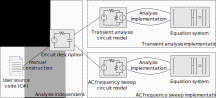
\includegraphics[width=\linewidth]{library-workflow}
	\caption{Workflow used in NextGen SPICE library}
	\label{fig:library-workflow}
\end{figure}

\subsection{Devices and Device Models}
\label{chap:analysis:device-models}
We have also stated that we would like the possibility of adding a new devices in the future. To achieve that, transient analysis (and each other analysis to be implemented) should specify operations required from each device via an interface. Adding new device would consist of implementing this interface for each analysis type. Figure~\ref{fig:analysis-interface} illustrates a possible device implementation hierarchy. Suppose that transient analysis requires the \texttt{ITransientDevice} interface, and AC frequecy sweep requires the \texttt{IAcFreqSweepDevice} interface. We have already described that capacitor and inductor devices are handled differently in both of these analyses, and it would make sense to implement the behavior separately for each analysis. At the same time, some devices -- such as resistors -- are handled the same way. The implementation of the resistor device could possibly implement both interfaces in the same class.

\begin{figure}[h]
	\centering
	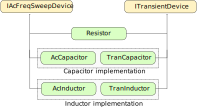
\includegraphics[width=0.7\linewidth]{analysis-interfaces}
	\caption{Implementation of devices for different circuit analyses}
	\label{fig:analysis-interface}
\end{figure}

Furthermore, we also stated in the requirements that it should be possible to easily change how each device is simulated. As an example, consider a BJT transistor device. During transient analysis, a BJT transistor can be modeled by using either the Ebers-Moll model or the more detailed Gummel-Poon model. Other analysis types can potentially use different transistor models. We would like to allow users to select which device model\footnote{To avoid possible confusion with \texttt{.MODEL} statements used in netlist files, this thesis uses term \textit{device model} exclusively to refer to the set of equations describing the device's behavior (such as the mentioned Ebers-Moll model). The entities described by \texttt{.MODEL} statement are referred to as \textit{device model parameters}.} should be used for the BJT device (and other devices as well). This will allow the library to be used for comparing existing device models and developing new ones. A concrete example hierarchy of the classes, which can be used to model a BJT transistor in transient and AC frequency sweep analyses, is illustrated in figure~\ref{fig:analysis-separation}. The classes \texttt{TranEbersMollBjt} and \texttt{TranGummelPoonBjt} implement the operations required by transient analysis for the respective transistor device models. During AC freqency sweep analysis, a completely different model (Hybrid-pi) is used, which is implemented by the \texttt{AcHybridPiBjt} class.

\begin{figure}[h]
	\centering
	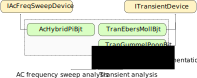
\includegraphics[width=.7\linewidth]{transient-separation}
	\caption{Separation of device implementation for each analysis type.}
	\label{fig:analysis-separation}
\end{figure}


\subsection{Splitting to Multiple Assemblies}
\label{chap:analysis:splitting}

A straightforward way of implementing the library would be putting everything into one assembly. However, that means that after each modification, the whole library has to be replaced by the new version. In the preceding section we decided to make the implementation of individual analysis types independent of each other, with a separate set of classes for representing the circuit under analysis. As developers, we would like to be able to develop, update and deploy each type of circuit analysis independently of the other types. In order to achieve that, we decided to organize the library into assemblies as illustrated in figure~\ref{fig:library-modules}. The \texttt{NextGenSpice.Core} is a shared assembly containing analysis-independent parts of the library, and is referenced by assemblies implementing individual analysis types. The implementation of the circuit model for transient analysis will be contained in the \texttt{NextGenSpice.LargeSignal} assembly. We chose the name LargeSignal because the resulting model allows transient, DC sweep and DC operating point analyses, which all rely on the large-signal model of circuit devices.

\begin{figure}[h]
	\centering
	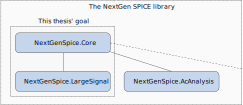
\includegraphics[width=0.8\linewidth]{analysis-modules}
	\caption{General organisation of the analysis types in the library.}
	\label{fig:library-modules}
\end{figure}

The \texttt{NextGenSpice.Core} assembly should have no knowledge of the assemblies containing the analysis types. To achieve that, we will make use of a principle called \textit{inversion of control} (IoC). In simple words, each assembly containing the implementation of a circuit analysis type should inform the \texttt{NextGenSpice.Core} assembly of its existence and instruct it how its circuit model can be created from the circuit description.

To make this procedure automatic without any action needed from the library's user, we decided to use an IoC framework. The functionality we require from the framework is quite simple and available in most IoC frameworks (importing implementations of certain interface from assemblies in the same directory as the core library). We decided to use the MEF framework \cite{mef} by Microsoft, which is distributed as a NuGet package and is standardly used. Another attractive feature of MEF is that it allows exporting classes by simply adding an \texttt{[Export]} attribute. 

In this section we described the reasons for the overall design of the NextGen SPICE library; in the sections that follow, the individual components of the library are analyzed in greater depth.

\section{NextGenSpice.Core}

The \texttt{NextGenSpice.Core} assembly will be the integral part of NextGen SPICE. It should contain the analysis-independent parts of the library: the circuit description classes, faculties for composing and validating the circuit, and the central mechanism that allows creation of analysis-specific circuit models. These parts will be discussed in the following subsections.

\subsection{Representation of the Circuit}
\label{fig:analysis:representation-circuit}
In the previous section we made the important decision to introduce separate sets of classes for circuit representation for each circuit analysis type. We have also decided to create another separate circuit description from which these analysis-specific representations should be constructed on-demand. The circuit description should be encapsulated in a single object of class \texttt{CircuitDefinition} for easy manipulation. The following subsubsections consider individual aspects of representing the circuit.

\subsubsection{Representing Circuit Nodes} 
In the SPICE netlist syntax, as described in chapter~\ref{chap:spicecode}, we allow circuit nodes to be identified by arbitrary alphanumeric strings, which would make the C\# type \texttt{string} a straightforward choice.

However, the main reason for using strings in the netlist syntax was probably to let users choose convenient names and make the netlists more readable. During the actual simulation and equation formulation, the circuit nodes need to be numbered in order to map the devices to corresponding equation matrix entries, and it would be more natural to use numbers to identify the circuit nodes. 

Because we do not expect users of the NextGen SPICE library to compose large circuits in the source-code manually, we decided to use the C\# type \texttt{int} for identifying individual nodes. This also implies that we need to translate circuit node names while parsing SPICE netlists into node indices, and provide this mapping to the user.

\subsubsection{Representing Individual Devices}
\label{chap:analysis:representation}
We need a circuit device representation which allows simple adding of new devices. A natural way of representing cicruit devices in an OOP language like C\# is introducing a class per circuit device, which all implement the same interface, e.g. \texttt{ICircuitDefinitionDevice}. This would lead to a hierarchy parallel to that of the analysis-specific device implementation classes from section~\ref{chap:analysis:device-models}. Having these multiple parallel hierarchies would simplify implementation of the analysis-specific circuit model creation, because all it would need is a mapping between these two hierarchies, as illustrated in figure~\ref{fig:03-fig-definition-hierarchy}.

\begin{figure}[h]
	\centering
	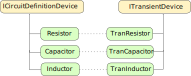
\includegraphics[width=0.57\linewidth]{definition-hierarchy}
	\caption{Mapping between circuit definition and analysis implementation classes}
	\label{fig:03-fig-definition-hierarchy}
\end{figure}


All data specific for any particular device would be stored in the respective properties of the device's class, and new devices can be added by creating another implementation of the \texttt{ICircuitDescriptionDevice} interface. Since this circuit device representation meets our requirements, we decided to use it.

\subsubsection{Representing subcircuits}
An important feature of SPICE netlists which we need to take into consideration when designing the circuit representation is the subcircuit feature (see section~\ref{chap:spicecode:subcircuits}).

Since a subcircuit can be used multiple times throughout a netlist file (i.e.\ multiple \texttt{X} statements with the same subcircuit name), we have decided to create separate classes \texttt{SubcircuitDefinition} for the description of the subcircuit  and \texttt{SubcircuitDevice} for the usage of the subcircuit. The subcircuit definition would need to store data about the inner devices and nodes, and which nodes are the connections to the outside circuit. The \texttt{SubcircuitDefinition} instances would be shared among potentially many \texttt{SubcircuitDevices}, which store data about the outside nodes to which the subcircuit is connected. 

%\todo{figure?}

\subsubsection{Enforcing Circuit Topology}
In section~\ref{chap:spicecode:topology}, we described circuit topology restrictions that we will impose on the circuit to ensure that the circuit equations during the simulation have a unique solution. Also, we want to prohibit the user from making changes to the circuit topology during the circuit simulation, because it could cause the circuit to be no longer valid. We would also like to diagnose any circuit topology violations as soon as possible, preferably immediately after the whole circuit is constructed.

Changes to the circuit topology could be achieved by two ways: adding or removing a whole device, and changing the nodes to which the device was connected. Both can be forbidden by making the circuit description read-only. However, that would mean that all circuit devices would have to be supplied at once to the \texttt{CircuitDefinition} constructor, and the validation would have to be performed inside the constructor.

To move the validation code outside the \texttt{CircuitDefinition} class, we will use a separate class \texttt{CircuitBuilder} to incrementally add new devices, and perform the validation before creating the actual \texttt{CircuitDefinition} class instance.

\subsection{Creating Analysis-specific Circuit Representations}
Back in section~\ref{chap:analysis:separation}, we decided to introduce multiple parallel hierarchies for representing the electrical circuit, each one for a particular circuit analysis. In order for the library to be easy to use, the user should not have to create these representations separately for each circuit analysis type manually. Instead, the library should provide a way to create the analysis-specific circuit representations automatically.

An ideal user interface of the library would allow the user to specify a mapping between the circuit description classes as discussed in section~\ref{chap:analysis:representation}. If the user then requested the transient analysis circuit representation, the library would then use this mapping to instantiate classes that implement the transient analysis logic for each device from the circuit description, and return the result back to the user.

This mapping will also be used to specify which device model should be used during the analysis. To allow simple comparing of different device models (such as the Ebers-Moll or Gummel-Poon BJT transistor models, which would each be implemented as a separate class, as discussed back in section~\ref{chap:analysis:device-models}), we would like to allow users to potentially specify multiple sets of mappings for a certain analysis type.

We have therefore decided to encapsulate these mappings in a \textit{factory class}. However, the concrete class type of the analysis-specific circuit representation is not known, because the \texttt{NextGenSpice.Core} assembly does not contain any analysis-specific functionality. We will therefore use a class hierarchy similar to the one in figure~\ref{fig:analysis-model-factories}. We will use the generic class feature of C\# and implement an abstract \texttt{AnalysisModelFactory<T>} class with one generic parameter for the circuit representation class type. This abstract class will implement methods for managing the mappings between a device description and implementation classes (symbolized by the \texttt{SetModel} method). The actual instantiation of the analysis-specific circuit model (\texttt{LargeSignalCircuitModel} on the figure) is delegated to derived classes, which provide a way to create new methods by implementing the abstract \texttt{NewInstance} method.

\begin{figure}[h]
	\centering
	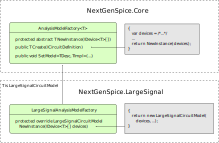
\includegraphics[width=0.9\linewidth]{analysis-factories}
	\caption{Relationship between analysis model factories}
	\label{fig:analysis-model-factories}
\end{figure}

In section~\ref{chap:analysis:splitting}, we decided to use the MEF framework to automatically discover the available analysis types. This means that each assembly with a circuit analysis implementation needs to export its own class derived from \texttt{AnalysisModel\+Factory<T>}. To provide a convenient place to aggregate the exported factories, we introduced yet another class: \texttt{AnalysisModelCreator}, which serves as a container for the analysis circuit model factories. The actual analysis model creation can be then implemented as a generic method on \texttt{AnalysisModelCreator}, which will then find the appropriate factory to be used for the construction of the desired circuit model class specified as the type argument.

\section{SPICE Netlist Parser}
\label{chap:analysis:parser}
An important feature of our library is to allow users to import subcircuits from SPICE netlist files (Goal~\ref{goal:parser}). Therefore, a SPICE netlist parser needs to be implmented.

Both the lexer and parser can be either written manually or be generated by a tool. In .NET ecosystem, possible choices include tool generators such as ANTLR \cite{antlr}. When using these generator tools, the language is described by a set of regular expressions and formal grammar rules, and the tool then generates the implementation of the lexer and parser.

Since the SPICE netlist grammar has a simple structure and a hand-written parser would be easy to write, we have come to the conclusion that the generator tools would only add unnecessary complexity to the library's implementation, and we will therefore implement the parser manually. 

\section[Double-double and Quad-double Arithmetic]{Double-double and Quad-double \\ Arithmetic}
\label{chap:analysis:dd}
According to goal~\ref{goal:dd} of this thesis, the library should allow representing real numbers with greater precision using the double-double and quad-double technique. The implementation of these techniques is very complex and requires deep knowledge and understanding of the algorithms to be done correctly. Therefore, we will not implement double-double and quad-double arithmetic ourselves, but we will use a third party library to provide that functionality.

During our search for a suitable library, we did not find any implementation of double-double or quad-double in .NET. However, we discovered a C++ implementation by Hida et al. called QD \cite{qd-lib} which is available under the BSD license. Even though our library will be targeted at .NET Standard, we still can use this library because .NET Standard version 2.0 requires implementations of .NET to provide PInvoke, which is a feature that allows making calls to native code.

Because C++ is a compiled language, the implementation of QD needs to be recompiled for each platform, which would complicate the deployment of the library. However, the enhanced precision is needed only while solving a circuit equation, where the truncation errors could cause significant errors in the solution. A standard \texttt{double} type is sufficient for storing the parameters of the individual circuit devices. This means that enhanced types are not needed in the simulator's interface, but can be a detail of the equation system implementation, which can be changed without affecting the user's code.

We have therefore decided to use a different internal real number representation based on compile time compilation symbols. When no symbols are specified, the library would be compiled without any dependencies on the native code (and hence use the \texttt{double} type). The library thus compiled can be distributed just like any .NET Library. On the other hand, users who wish to use enhanced precision types can still do so by compiling the library with appropriate symbols.

Using a C++ implementation of individual arithmetic operations on the double-double and quad-double types also means that a call to native code has to be made for each numeric operation during equation solution. The transition between managed and unmanaged code for such trivial operations may incur nontrivial overhead. To gain better insight on how significant this overhead would be in our implementation, we implemented Gaussian elimination on the \texttt{double} type in four variants.

\begin{itemize}
	\item \texttt{Managed} -- normal implementations in C\# code.
	\item \texttt{Managed\_Wrapped} -- the \texttt{double} type was wrapped in a struct that implements necessary arithmetic operators by built-in operators on the \texttt{double} type. This implementation reflects more closely how the double-double and quad-double types would perform when implemented in pure .NET.
	\item \texttt{Managed\_Pinvoke} -- similar to \texttt{Managed\_Wrapped}, but the arithmetic operations are performed in C++ via a PInvoke call. This is how the enhanced precision types will perform when PInvoke is used for each arithmetic operation.
	\item \texttt{Native} -- The whole algorithm is implemented in C++ and performed on one PInvoke call.	
\end{itemize}

We used BenchmarkDotNet \cite{benchmarknet} for measuring the run times for equation systems. The  table in figure~\ref{fig:gauss-benchmark} summarizes the results on equation systems with $N$ variables for $N = 20$ and $200$ variables. All times are in microseconds.\footnote{The benchmarks were run on system with i5-6300HQ 2.30 GHz CPU using .NET Core 2.0.6 (CoreCLR 4.6.26212.01, CoreFX 4.6.26212.01), 64bit RyuJIT, Release mode.}

\begin{figure}[h]
	\centering
	\begin{tabular}{|r|r|r|r|r|r|}
		\hline
		Method & N & Mean ($\mu{}s$) & Error ($\mu{}s$) & StdDev ($\mu{}s$) & Scaled  \\ \hline \hline
		         \texttt{Managed} &  20 &      7.900  &   0.0147  &   0.0114  &   1.00  \\ \hline
\texttt{Managed\_Wrapped} &  20 &     27.233  &   0.1208  &   0.1070  &   3.45  \\ \hline
\texttt{Managed\_Pinvoke} &  20 &     91.116  &   0.3146  &   0.2789  &  11.53  \\ \hline
\texttt{Native} &  20 &      3.446  &   0.0167  &   0.0156  &   0.44   \\ \hline \hline
\texttt{Managed} & 200 &  6,242.546  &  25.2918  &  22.4205  &   1.00  \\ \hline
\texttt{Managed\_Wrapped} & 200 & 22,026.703  &  97.9251  &  91.5992  &   3.53  \\ \hline
\texttt{Managed\_Pinvoke} & 200 & 83,690.755  & 550.2520  & 487.7840  &  13.41 \\ \hline
\texttt{Native} & 200 &  2,413.073  &   5.9563  &   5.5715  &   0.39  \\ \hline
	\end{tabular}
	\caption{Benchmark results for Gaussian elimination implementation.}
	\label{fig:gauss-benchmark}
\end{figure}

These results show that the overhead of PInvoke would be certainly noticeable if it were used for all arithmetic operations and could slow down the simulation by as much as an order of magnitude. To provide a way to avoid this overhead, we will implement the numeric routine for solving the equation system in both .NET and C++. This way, the transition between runtimes would occur only once per equation system solution. The choice of whether the managed or native version would be used will depend on another conditional compilation symbol.

\section{NextGenSpice.LargeSignal}

The \texttt{NextGenSpice.LargeSignal} assembly contains the implementation of transient analysis, the implementation of which we set as goal~\ref{goal:transient}. To understand the motivation for choices made in our analysis, we first describe the process of transient analysis in greater detail. Then we proceed with the actual implementation analysis of transient analysis in the NextGen SPICE library.

\subsection{Transient Analysis Overview}
\label{chap:analysis:transient-overview}
Transient analysis models the circuit's behavior over time. It is used to calculate the values of node voltages and currents flowing through the circuit network (which is shortly referred to as the \textit{DC bias} of the circuit) at specified timepoints in the simulated period. The top-level illustration of the simulation algorithm is shown in figure~\ref{fig:analysis-transient-top-level}.

\begin{figure}[h]
	\centering	
	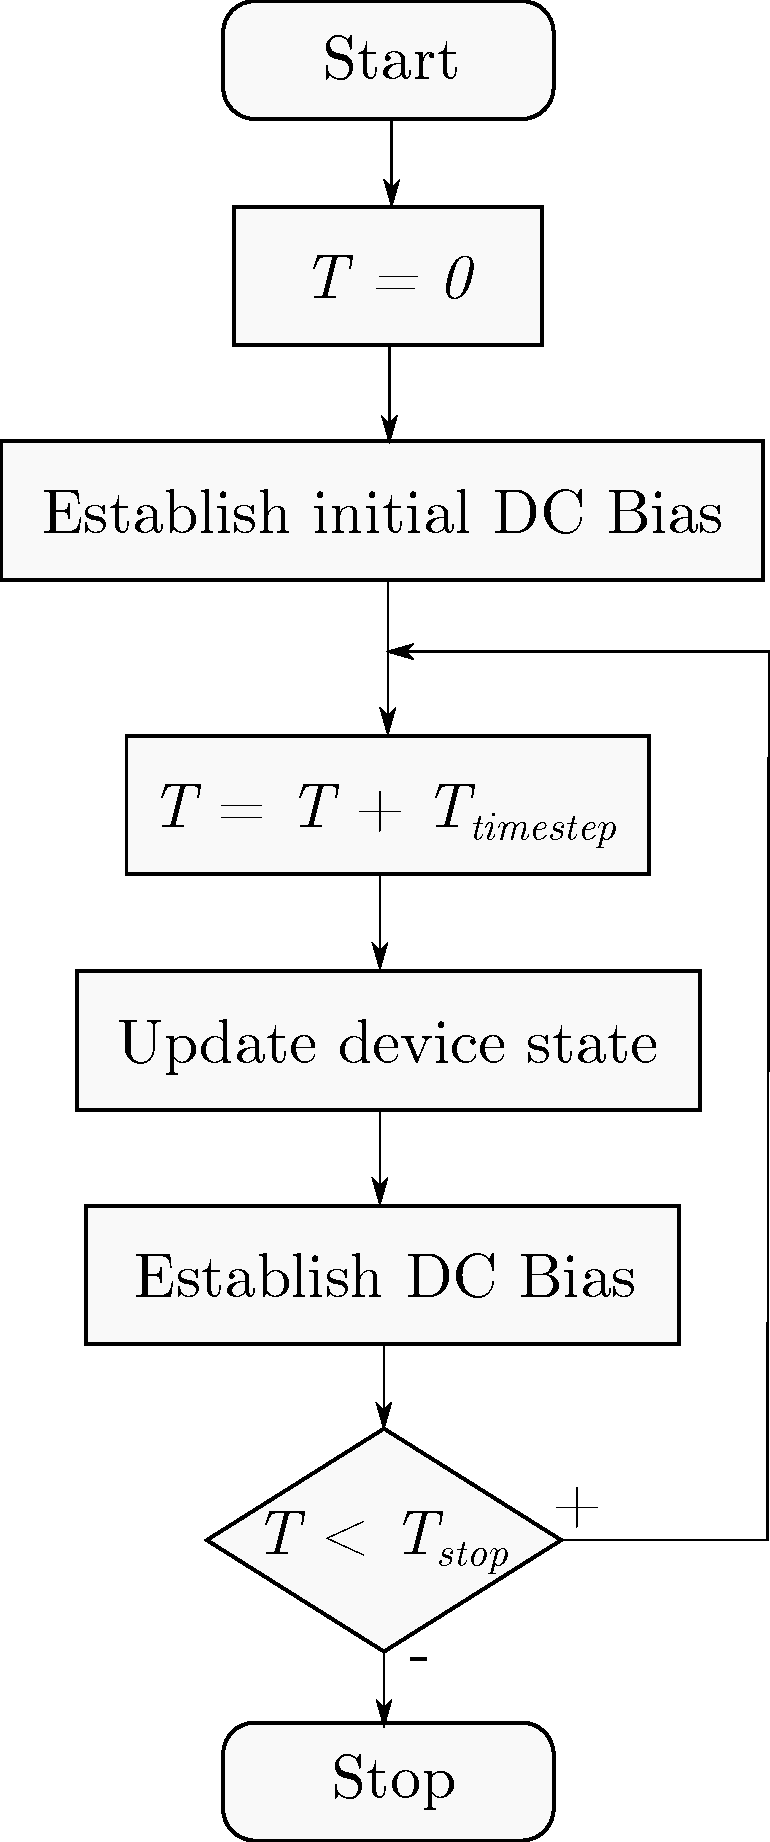
\includegraphics[width=.3\linewidth]{transient-analysis-diagram}
	\caption{Top level description of the transient analysis algorithm}
	\label{fig:analysis-transient-top-level}
\end{figure}

The simulation starts by calculating the initial DC bias of the circuit, during which capacitor and inductor devices are modeled as ideal open circuits and closed circuits, respectively. After the initial state of the circuit is established, the state of of active devices like capacitors and inductors, or nonconstant voltage and current sources is updated to reflect the time passed between the two successive timepoints. To reflect the energy stored in the capacitor and inductor devices, these devices are replaced by so called \textit{companion models}, which consist of either voltage or current source and a resistor. Parameters of the devices in the companion models are recomputed in each succesive timepoint (technical details will be explained later). Then a DC bias calculation is performed for the next timepoint and the process is repeated for the whole simulated period.

The details of DC bias calculation are described in the following subsections.
\subsubsection{DC Bias Calculation} 

We will demonstrate the DC bias calculation on the circuit shown in figure~\ref{fig:analysis:ls-bias-circuit}. Different colors of the devices will serve a purpose later.

\begin{figure}[h]
\begin{circuitdev}
	(0,0) 
	to[V=12<\volt>,invert,color=red] (3,0) node[circ,label={-90:$1$}]{}
	-- (6,0)
	to[R, l=5<\ohm>, ,color=blue] (6,3) node[circ,label={3:$3$}]{}
	to[R, l=5<\ohm>, color=green] (3,3) node[circ,label={$2$}]{}
	to[R, l=10<\ohm>, color=orange] (0,3)
	-- (0,0)
	
	(3,0) to[R, l=10<\ohm>,color=purple] (3,3)
	(0,1.5) -- (-0.5,1.5) node[ground]{}
\end{circuitdev}	
	\caption{Example circuit for DC bias calculation.}
	\label{fig:analysis:ls-bias-circuit}
\end{figure}


To calculate the node voltages and branch currents, the equations corresponding to the Kirchhoff's circuit laws must be formulated. There are several methods for algorithmic formulation of the circuit equations. As an example, we will show the \textit{Modified Nodal Analysis} (MNA) method. In MNA, there is a template for each device type's contribution to the equation system, which is called a device's \textit{stamp}. Device stamps for constant voltage source and resistor are shown in figure~\ref{fig:device-stamps}. An important thing to notice is that voltage sources (and some other devices) require an additional variable in the equation system for calculating the current flowing through the device.

\begin{figure}[h]
		\centering
		\begin{circuitdev}
			(0,0) node[label=N+]{} to[V, l=V, *-*, i_>=$I_V$] (3,0) node[label=N-]{}
			
			
			(9,0) node[label=N+]{} to[R, l=R, *-*] (12,0) node[label=N-]{}
		\end{circuitdev}
\[\begin{bmatrix}
	 &  & 1  \\
	 &  & -1 \\
	1 & -1 & 
\end{bmatrix} \cdot 
\begin{bmatrix}
V_{N+}\\
V_{N-}\\
I_V
\end{bmatrix}
=
\begin{bmatrix}
 \\
 \\
 V
\end{bmatrix}
\qquad
\qquad
\qquad
\begin{bmatrix}
	\frac{1}{R}& -\frac{1}{R}  \\
-\frac{1}{R}	& \frac{1}{R} \\
	\end{bmatrix}
\cdot
\begin{bmatrix}
V_{N+}\\
V_{N-}\\
\end{bmatrix}
=
\begin{bmatrix}
	\\
	\color{white}{f}
\end{bmatrix}\]
	\caption{Device stamps for the voltage source and resistor}
	\label{fig:device-stamps}
\end{figure}

Formulation of the circuit using MNA is done by iterating through the list of circuit devices and "stamping" them into the equation system. When applied to the circuit in figure~\ref{fig:analysis:ls-bias-circuit} MNA creates the following equation system shown in figure~\ref{fig:equation-example}. The contribution from each device is shown in the same color as the device.

\begin{figure}[h]
	\centering
	\[
	\color{black}
	\begin{bmatrix}
	\mathcolor{orange}{\frac{1}{10}}	&0	&	\mathcolor{orange}{-\frac{1}{10}}  	&0 	&0	& 0 \mathcolor{red}{-1}\\
	0	&	\mathcolor{purple}{\frac{1}{10}} + \mathcolor{blue}{\frac{1}{5}}	&	\mathcolor{purple}{-\frac{1}{10}}  	& \mathcolor{blue}{-\frac{1}{5}}	&0	&  \mathcolor{red}{1}\\
	\mathcolor{orange}{-\frac{1}{10}}	&	\mathcolor{purple}{-\frac{1}{10}}	&	\mathcolor{orange}{\frac{1}{10}} + \mathcolor{purple}{\frac{1}{10}} + \mathcolor{green}{\frac{1}{5}} 	&  \mathcolor{green}{-\frac{1}{5}} 	&0 & 0  \\
	0	&\mathcolor{blue}{-\frac{1}{5}}	& \mathcolor{green}{-\frac{1}{5}} 	& \mathcolor{blue}{\frac{1}{5}} + \mathcolor{green}{\frac{1}{5}} &0	&0 \\
	\mathcolor{red}{-1}	& \mathcolor{red}{1}	&0  	&0 	&0	&0
	\end{bmatrix} \cdot 
	\begin{bmatrix}
	V_0\\
	V_1\\
	V_2\\
	V_3\\
	\mathcolor{red}{I_V}
	\end{bmatrix}
	=
	\begin{bmatrix}
	0\\
	0\\
	0\\
	0\\
	\mathcolor{red}{12}
	\end{bmatrix}
	\]
	\caption{Equation system after stamping devices from our circuit}
	\label{fig:equation-example}
\end{figure}

Because node 0 corresponds to the ground node, it always holds that $V_0 = 0$. Therefore, the corresponding row and column can be eliminated. By solving the resulting equation system, we obtain the values $V_1 = 12$, $V_2=10$, $V_3=8$ and $I_V=-0.8$. Branch currents flowing through the resistors can be then trivially calculated using the formula $I_R = U_R/R$. 

\subsubsection{DC Bias Calculation - Nonlinear Devices}
In the preceding example, only \textit{linear} devices were used in the circuit. This means that the resulting equation system was also linear and an exact solution could be obtained. Another situation arises if a nonlinear device such as diode is used in the circuit. A semiconductor diode has nonlinear I-V characteristic which is approximated by the Shockley equation shown in figure~\ref{fig:diode-iv}.

\begin{figure}[h]
	\centering
	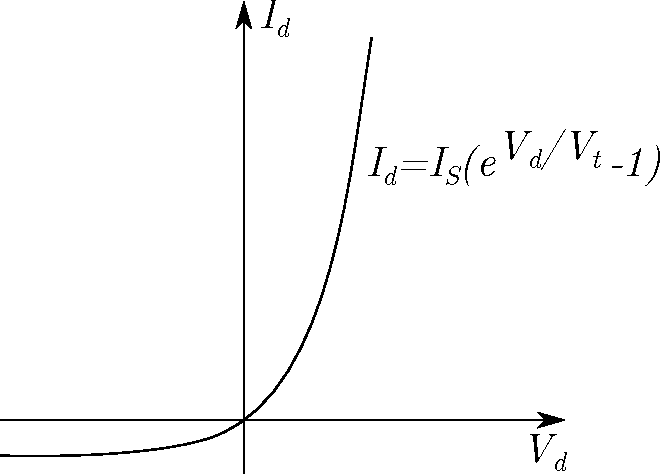
\includegraphics[width=0.32\linewidth]{diode-iv}
	\caption{I-V characteristic of a diode}
	\label{fig:diode-iv}
\end{figure}

Circuits containing such devices can no longer be characterized by a system of linear equations. Instead, a system of nonlinear equations needs to be solved. Such systems are solved iteratively by the Newton-Raphson method. In DC bias calculation, the Newton-Raphson algorithm is realized by repeatedly linearizing the I-V characteristics of nonlinear devices at the current candidate DC bias and solving the linearized equation system, to obtain the next candidate DC bias. Figure~\ref{fig:diode-equivalent} shows the linearization process on the diode example from figure~\ref{fig:diode-iv} around $V_B$, which is a current guess of the voltage across the diode. The linearized I-V characteristic then corresponds to replacing the diode by an \textit{equivalent circuit} consisting of a current source with $ I_{eq} $ current and a resistor with $ G_{eq} $ conductance, as shown in the figure.

\begin{figure}[h]
	\centering
		\begin{subfigure}{0.32\linewidth}
			\centering
			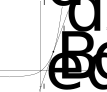
\includegraphics[width=\linewidth]{linearizing-diode}
		\end{subfigure}
		\begin{subfigure}{0.65\linewidth}
			\centering
			\begin{circuitdev}
				(-1.5,0) node[circ,label=1:+]{} to[D,i=$I_d$] (-1.5,-4) node[circ, label=1:-]{}
				
				(4,0) node[circ, label=1:+]{} -- (4,-0.5) -- (3,-0.5) to[I, a=$I_{eq}$] (3,-3.5) -- (4,-3.5) -- (4,-4) node[circ, label=1:-]{}
				
				(4,-0.5) -- (5,-0.5) to[R, l=$G_{eq}$] (5,-3.5) -- (4,-3.5);
				
					\draw [decoration={markings,mark=at position 1 with
					{\arrow[scale=3,>=stealth]{>}}},postaction={decorate}] (-0.5,-2) -- (1,-2)
			\end{circuitdev}
		\end{subfigure}
	\caption{Linear equivalent circuit for the diode}
	\label{fig:diode-equivalent}
\end{figure}

This iterative process stops when the difference between the diode currents in two consecutive solutions fits in the relative and absolute tolerances, which are parameters of the simulation. Another simulation parameter is the upper limit on the number of Newton-Raphson iterations. If the solution does not converge by the specified limit, then the simulation is aborted.

\subsubsection{DC Bias Calculation - Energy Storage Devices}

We have already briefly mentioned at the beginning of the subsection that capacitor and inductor devices are modeled by their companion models, which characterize the I-V characteristic of the device for the current timepoint. Figure~\ref{fig:capacitor-equivalent} shows the companion models for capacitor and inductor devices.

\begin{figure}[h]
	\centering
	\begin{subfigure}{0.49\linewidth}
		\centering
		\begin{circuitdev}
			(-0.5,0) node[circ,label=1:+]{} to[C] (-0.5,-4) node[circ, label=1:-]{}
			
			(4,0) node[circ, label=1:+]{} -- (4,-0.5) -- (3,-0.5) to[I] (3,-3.5) -- (4,-3.5) -- (4,-4) node[circ, label=1:-]{}
			
			(4,-0.5) -- (5,-0.5) to[R] (5,-3.5) -- (4,-3.5);
			\draw [decoration={markings,mark=at position 1 with
				{\arrow[scale=3,>=stealth]{>}}},postaction={decorate}] (0.5,-2) -- (2,-2)
		\end{circuitdev}
		\subcaption{Capacitor}
	\end{subfigure}\begin{subfigure}{0.49\linewidth}
			\centering
		\begin{circuitdev}
			[white] (0.5,0)  to[V,color=white] (0.5,-4); \draw
			
			(0.5,0) node[circ,label=1:+]{} to[L] (0.5,-4) node[circ, label=1:-]{}
			
			(4,0) node[circ, label=1:+]{} to[R] (4,-2) to[V, invert] (4,-4) node[circ, label=1:-]{};
			
			\draw [decoration={markings,mark=at position 1 with
				{\arrow[scale=3,>=stealth]{>}}},postaction={decorate}] (1.5,-2) -- (3,-2)
		\end{circuitdev}
		\subcaption{Inductor}
	\end{subfigure}
	\caption{Companion models of capacitor and inductor}
	\label{fig:capacitor-equivalent}
\end{figure}

Parameters of the companion models are updated each timepoint via \textit{numerical integration} to reflect the energy stored in the device. However, if the timestep used in the simulation is too big, local errors made during the integration may accumulate and therefore produce unrealistic results of the simulation. On the other hand, smaller timestep means that the simulation will take longer. Modern simulators internally choose the timestep dynamically: small timestep values when the values of companion models change rapidly, and greater timestep values otherwise. This way the simulator preserves both speed and accuracy. This process is illustrated in figure~\ref{fig:dynamic-timestep}.

\begin{figure}[h]
	\centering
	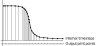
\includegraphics[width=.8\linewidth]{dynamic-timestep}
	\caption{Depiction of dynamic timestep mechanism, reproduced from Inside SPICE \cite{inside_spice}}
	\label{fig:dynamic-timestep}
\end{figure}

This process is realized by iterating individual devices and estimating the maximum timestep for which the truncation error does not exceed the simulator tolerances. The minimum of these values is then chosen as the next timestep. 

To implement transient analysis as described so far, we need to make important decisions regarding individual parts of the algorithm. The main parts that need to be analyzed are the method used for equation system formulation, representation of the equation system, choice of numerical integration method, choice of timestep control mechanism and the interface that will be required from device logic implementations.

\subsection{Choice of Equation System Formulation}

As we mentioned in the previous subsection, there are several methods for automated creation of the circuit equation system. Many of those are described in great depth in Nagel's PhD thesis \cite{Nagel:M520}, chapter III. 

Nagel includes a comparison of the methods with respect to the size of the equation and the programmatic effort of implementing these methods. His research shows that the MNA method which was used in the example in section~\ref{chap:analysis:transient-overview} produces comparatively smaller equation systems than other methods. 

Another advantage of using the MNA method is that it does not require finding loops and trees in the circuit graph, which are required by methods like Modified Tableau Analysis. Instead, as we have shown earlier, all devices contribute to the equation system via a device type stamp. Also, adding a new device type does not require changes to the formulation method, because the device stamp can be made part of the device's implementation.

For the reasons above, we decided to use the MNA method during transient analysis.

\subsection{Equation System Abstraction}
\label{chap:analysis:equation}
There are multiple ways of representing the equation system. The most straightforward way is representing the equation matrix as a full two-dimensional array. Such a representation is intuitive and easy to manipulate in the program. However, if the equation matrix is sparse (many coefficients are equal to 0), this representation is inefficient. When using MNA, the number of nonzero elements in a row is roughly proportional to the number of devices that connect to that node. This means that in large circuits, where only a small number of devices connects to the same node at once, it would be more appropriate to use a sparse matrix representation.

We decided to use the full 2D array representation for simplicity, but in case that this representation would prove to be an issue in the future, we would like to change the implementation without affecting the user code. Therefore, we have to expose the equation system under an interface that can be efficiently implemented by sparse matrix representations too.

There is also an additional requirement on the equation system implementation. As we have shown in figure~\ref{fig:device-stamps}, devices may need an additional circuit variable to be correctly simulated. The equation system implementation therefore needs to support adding additional variables at least during the initialization phase of the simulation.

Because we decided to use the MNA method for equation system formulation, each device needs to modify only a small fixed set of equation system coefficients corresponding to the device's stamp. We have therefore decided to use the interface illustrated in figure~\ref{fig:analysis-equationsystem}. During the initialization phase of the simulation, each device would request any number of additional variables that it requires, and specify which equation system coefficients it contributes to. Access to these coefficients will be then provided using a proxy object for each accessed coefficient. 

\begin{figure}[h]
	\centering
	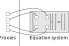
\includegraphics[width=0.4\linewidth]{analysis-equationsystem}
	\caption{Equation system abstraction}
	\label{fig:analysis-equationsystem}
\end{figure}

This interface is general enough to allow any internal equation system representation while providing efficient access to individual coefficients.

\subsection{Choice of Numerical Integration Method}
In the description of transient analysis of energy storage devices, we mentioned that the inner state of the device is updated based on the circuit state of the previous timepoint using numerical integration. Commonly used integration methods include Backward Euler, Trapezoidal Rule, and Gear method. A summary of these and other numerical integration methods can be found in QUCS Technical Papers, section 6.1. Nagel's PhD thesis also provides a detailed analysis of common numerical integration methods in chapter VI. None of these methods can be considered best for circuit simulation. For example, although the trapezoidal rule is very good in terms of accuracy and speed, it may sometimes lead to a phenomenon called \textit{trapezoidal ringing}, which means that the value oscilates around the exact value. The trapezoidal ringing is shown in figure~\ref{fig:trap-ringing}.

\begin{figure}[h]
	\centering
	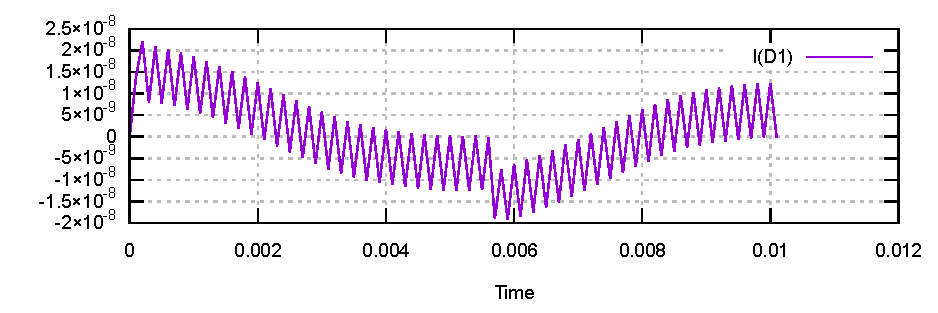
\includegraphics[width=0.8\linewidth]{04-fig-back-to-back-trap}
	\caption{Trapezoidal ringing.}
	\label{fig:trap-ringing}
\end{figure}

For this reason, modern circuit simulators implement multiple integration methods. If the default method proves inappropriate, the user can instruct the simulator to use a different method. We would therefore like to allow using different integration methods in our simulator, and even allow the user to add new integration methods.
%As a proof of concept, we will implement Backward Euler, Trapezoidal Rule and Gear integration methods. \todo{remove the last sentence?}

\subsection{Choice of Timestep}
\label{chap:analysis-timestep}
While describing the simulation of energy storage devices back in section~\ref{chap:analysis:transient-overview}, we briefly mentioned that additional precision can be achieved by choosing the timestep dynamically. The dynamic methods choose the timestep such that the error introduced by the integration method is less than a certain threshold. The timestep choice therefore depends on the integration method and the device's state in previous timepoints.

We decided to simplify the library's implementation and not implement the dynamic timestep in the initial version of the library. Therefore, the library will rely on the user to specify an appropriate timestep value that will be used throughout the simulation. However, the dynamic timestep is an attractive feature and we would like to add it in the next versions of the library.

\chapter{Developer Documentation}

The implementation of the NextGen SPICE library is contained in one Visual Studio 2017 solution which consists of 10 projects; the overall structure of the solution is illustrated in figure~\ref{fig:solution-structure}.

\begin{figure}[h]
	\centering
	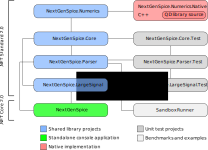
\includegraphics[width=0.87\linewidth]{solution-structure}
	\caption{Project structure of the solution}
	\label{fig:solution-structure}
\end{figure}

The \texttt{NextGenSpice.Core} project is the core project of the library, it contains classes for creating and validating electrical circuits. It also contains code that automatically discovers available analysis types through the MEF framework, and constructs analysis-specific circuit models from circuit description.

The \texttt{NextGenSpice.LargeSignal} project contains the implementation of the large-signal circuit model which allows performing DC operating point and transient analyses.

The \texttt{NextGenSpice.Parser} project contains the implementation of the SPICE netlist parser and allows users of the library to import circuits, subcircuits and device model parameters into the simulator.

The \texttt{NextGenSpice.Numerics} project defines classes for creating and representing equation systems for the simulator, as well as other mathematical functions that are needed in the simulator. It also serves as a managed wrapper around the \texttt{NextGenSpice.Numerics.Native} C++ project, which is used to build the QD library for double-double and quad-double arithmetic, and expose its methods to managed (C\#) code.

\texttt{NextGenSpice} represents the standalone console application, the implementation of which was the goal~\ref{goal:app} of this thesis. It is also the only library project which targets the .NET Core platform.

The other projects are not part of the distributed library or console application. The \texttt{SandboxRunner} console application project is used to run benchmarks for the circuit simulator, and the projects with \texttt{.Test} suffix contain unit tests for individual parts of the library.

\subsubsection{License}
The whole NextGen SPICE solution is provided under the MIT license. More details can be found in the \texttt{LICENSE.TXT} file in the solution folder (located in the \texttt{/sources} folder in the attached CD).

\section{Compilation}

To allow using enhanced precision types in the simulator library, the solution contains one C++ project (\texttt{NextGenSpice.Numerics.Native}), which potentially inhibits the portability of the library. As discussed in analysis section~\ref{chap:analysis:dd}, we decided that the use of C++ code should be conditional on the presence of compile time symbols. The use of native code depends on the conditional compilation symbols used when compiling the \texttt{NextGenSpice.Numerics} project. In Visual Studio 2017, these symbols can be set in Project Properties $\rightarrow$ Build $\rightarrow$ Conditional compilation symbols. The following table lists the symbols and their meaning for the compilation.


\newcolumntype{L}{>{\centering\arraybackslash}m{10cm}}
\begin{center}
	\begin{tabular}{|c|L|}
		\hline 
		Symbol & Precision type used \\ \hline \hline
		\texttt{dd\_precision}& Use the \texttt{dd\_real} type and double-double arithmetic \\ \hline 
		\texttt{qd\_precision}& Use the \texttt{qd\_real} type and quad-double arithmetic \\ \hline 
		\textit{no symbol} & Use the \texttt{double} type \\ \hline 
	\end{tabular}
\end{center}

\begin{center}
	\begin{tabular}{|c|L|}
		\hline 
		Symbol & Choice of Gauss elimination implementation \\ \hline \hline
		\texttt{native\_gauss}& Use native implementation  \\ \hline 
		\textit{no symbol} & Use managed implementation \\ \hline 
	\end{tabular}
\end{center}

The \texttt{NextGenSpice\+.Numerics\+.Native.dll} dll is defaultly compiled for 64-bit runtime. To use NextGen SPICE library in a 32-bit process, a 32-bit version of the  native dll must be compiled.

\section{NextGenSpice.Core}

The \texttt{NextGenSpice.Core} assembly contains the analysis independent parts of the NextGen SPICE library, namely the classes for circuit description, logic for validating the circuit, and a generic factory to be used for creating analysis-specific circuit models.

\subsection{Circuit Description}

In the analysis section~\ref{fig:analysis:representation-circuit}, we decided to represent the circuit description using a separate class for each device. These classes implement the \texttt{ICircuitDefinition\+Device} which defines the members \texttt{ConnectedNodes} and \texttt{GetBranchMetadata} which are used to validate the circuit topology. It also defines members \texttt{Tag} which can be used to identify individual devices and a \texttt{Clone} method for duplicating the device.

The \texttt{ConnectedNodes} property returns an instance of the \texttt{NodeConnectionSet} class which encapsulates the node connections. This class has \texttt{internal} setters, so that the connections are set only by the library and cannot be modified by the user.

\texttt{GetBranchMetadata} is used to retrieve the characteristics of the connections which are important for the circuit topology validation. The topology rules require that there is no cycle of voltage sources and inductors, and no cutset of current sources and capacitors. \texttt{GetBranchMetadata} therefore returns a collection of \texttt{CircuitBranchMetadata}  which contain information whether the device is \textit{current defined} or \textit{voltage defined}. If a device is neither (e.g.\ resistor), then the \texttt{GetBranchMetadata} returns an empty collection.

The circuit description is contained in the \texttt{CircuitDefinition} class, which simply wraps collection of \texttt{ICircuitDefinitionDevice} and provides other convenient methods (such as \texttt{FindDevice} to find a device by its tag). This class also has \texttt{internal} constructors, so that it can be created only by the library's code. The circuit definition is created by the \texttt{CircuitBuilder} class, which is also responsible for validating the circuit's topology.

The SPICE subcircuit representation consists of two parts: a \texttt{Subcircuit\+Definition} class which contains the description of the subcircuit in a similar manner as the \texttt{CircuitDefinition} class, and the \texttt{Subcircuit} class which implements the \texttt{ICircuitDefinitionDevice} interface and represents the subcircuit usage in the circuit. The \texttt{Subcircuit\+Definition} instances are shared among all coresponding \texttt{Subcircuit} classes.

\subsection{General Analysis Implementation Design}

Before we cover the mechanism which creates the analysis-specific circuit models from the circuit description, we will describe the interface hierarchies between the circuit description and analysis implementation. The \texttt{ICircuitDefinition} and \texttt{ICircuitDefinitionDevice} interfaces were described in previous subsection. The interfaces on the analysis implementation counterparts are \texttt{IAnalysis\+CircuitModel<TDevice>} and \texttt{IAnalysisDeviceModel<TAnalysis>}.

Because the relationship between these two interfaces is not trivial, we will explain them in the context of the large-signal analysis model implementation. Figure~\ref{chap:devdocs:analysis-design} shows the relationship between the classes and interfaces for circuit description and the large-signal circuit model.

\begin{figure}[h]
	\centering
	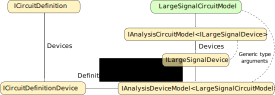
\includegraphics[width=.8\linewidth]{analysis-interface}
	\caption{Connection between the circuit description and analysis implementation}
	\label{chap:devdocs:analysis-design}
\end{figure}

The implementations of concrete analysis types are expected to extend the \texttt{IAnalysisDeviceModel} interface by adding methods required from the device's implementation. The additional methods for large-signal analysis are defined in \texttt{ILargeSignalDevice} which extends the \texttt{IAnalysisDeviceModel<LargeSignal\+CircuitModel>} interface. The generic argument in the \texttt{IAnalysisDeviceModel} interface is not used in the defined members, but provides metadata useful for enforcing that only the classes implementing \texttt{ILargeSignalDevice} interface can be registered as device models for \texttt{LargeSignalCircuitModel} (the model registration and analysis model factories will be covered in a later subsection). The \texttt{IAnalysisDevice\+Model} interface defines the \texttt{DefinitionDevice} property which serves as the link to the device from the original circuit description. The classes implementing the device-specific simulation logic will read the device's parameters from its definition device, which allows reacting to the changes of the device's parameters, as requested by goal~\ref{goal:transient}.

The \texttt{IAnalysisCircuit\+Model} interface has a generic parameter for the base type of the device's implementation, which is also the type of the items in its \texttt{Devices} property. The \texttt{LargeSignalCircuitModel} class requires each device to implement the \texttt{ILargeSignalDevice} interface. 

%The \texttt{TDevice} generic parameter must implement the \texttt{IAnalysisDeviceModel<IAnalysisCircuitModel<TDevice>>} interface, which enforces the fact that only

\subsection{Analysis Model Creation}

The creation of analysis-specific circuit models is done via a set of factories. Each analysis type assembly  (currently, only \texttt{NextGenSpice.LargeSignal} is implemented) exports an implementation of \texttt{IAnalysisModelFactory<T>} specialized on the class which will be used to represent the circuit for the particular analysis. In the case of \texttt{NextGenSpice.LargeSignal}, the class \texttt{LargeSignalAnalysisModel\+Factory} implements the \texttt{IAnalysisModelFactory<Large\+SignalCircuitModel>} interface and is used to build \texttt{LargeSignalCircuitModel} instances.

The core functionality for registering models for individual circuit devices is implemented in the abstract \texttt{AnalysisModelFactory<T>} class. The registering is done by calling the generic method \texttt{SetModel<TDesc, TImpl>} specialized on a definition device type and implementation device type. This function takes a factory function as a parameter, which will be later used to construct the implementation class. For example, the registering of \texttt{LargeSignal\+Resistor} as the implementation for \texttt{Resistor} device is done by calling

\begin{csharpcode}
IAnalysisModelFactory<LargeSignalCircuitModel> factory = /*...*/;
factory.SetModel<Resistor, LargeSignalResistor>(
	e => new LargeSignalResistor(e));
\end{csharpcode}

Thanks to the interface definitions as described in the previous section, it is possible to constrain the type arguments of the \texttt{SetModel} method to statically check that the \texttt{LargeSignalResistor} class implements \texttt{IAnalysisDeviceModel\+<LargeSignalCircuitModel>} interface (which it does by implementing \texttt{ILarge\+SignalDevice}). 

When a new circuit analysis model is to be created, all circuit devices from the \texttt{ICircuitDefiniton.Devices} collection are transformed by applying the supplied factory methods. The actual instantiating of the circuit model classes is delegated to the classes deriving from the \texttt{AnalysisModelFactory<T>} via the protected abstract method \texttt{CreateInstance}. In the implementation of the \texttt{LargeSignal\+AnalysisModelFactory}, this method return a new instance of the \texttt{LargeSignal\+CircuitModel} class.

\subsection{Discovering Analysis Model Implementations}

To simplify management of existing \texttt{IAnalysisModel\+Factory<T>} interface implementations, we introduced the \texttt{AnalysisModelCreator} class. This class defines the \texttt{Create<TAnalysis>} method, which finds the appropriate factory which to be used for creating the \texttt{TAnalysis} circuit model. The factory can be either registered manually using the \texttt{SetFactory<TAnalysis>} method, or automatically by adding \texttt{[Export(typeof(IAnalysisModelFactory<T>))]} attribute to the factory class. The implementation is then discovered by MEF framework.

To change the mapping between the circuit devices and their implementations, the respective factory can be obtained by the \texttt{GetFactory<TAnalysis>} method. \texttt{AnalysisModelCreator} also defines a static property \texttt{Instance} which holds the global singleton, however, it is possible to create multiple instances of this class and have different mappings in each instance. 

To simplify the library's interface for scenarios where only the global \texttt{Analysis\+ModelCreator} instance is needed, implementations of the circuit analyses are encouraged to define an extension function on \texttt{ICircuit\+Definition} which provides a simple way of creating analysis models using the global instance. For example, \texttt{NextGenSpice.LargeSignal} assembly defines the following extension method.

\begin{csharpcode}
public static LargeSignalCircuitModel
GetLargeSignalModel(this ICircuitDefinition definition)
{
	if (definition == null)
		throw new ArgumentNullException(nameof(definition));
	return AnalysisModelCreator.Instance
		.Create<LargeSignalCircuitModel>(definition);
}
\end{csharpcode}

\section{NextGenSpice.Parser}
As we stated in the analysis chapter in section~\ref{chap:analysis:parser}, we have decided to implement both the parser and lexer manually. The implementation is contained in the \texttt{NextGenSpice.Parser} project. The whole functionality is exposed through the instance methods of the \texttt{SpiceNetlistParser} class.

The class itself does not contain code for handling specific netlist statements, processing these statements is delegated to \textit{statement processors}, which will be described later in greater detail. A new instance of the parser can be obtained by the \texttt{SpiceNetlistParser.Empty()} method. The returned instance does not contain any statement processors, these would have to be registered manually. For convenience, the parser class contains a static method \texttt{SpiceNetlistParser\+.WithDefaults()}, which creates a new instance of the parser and automatically registers statement processors implemented as part of this thesis.

The parsing itself is done simply by calling the \texttt{Parse()} method, which accepts an instance of \texttt{TextWriter} class from which the netlist should be read. This method returns an instance of the \texttt{SpiceNetlistParser\+Result} class, which encapsulates all the information from the parsed file: \texttt{Circuit\+Description} for the contained circuit, collections of defined models and subcircuit, used node names, encountered errors etc.

All information regarding the netlist that is currently being parsed is aggregated in the \texttt{ParsingContext} class. This class contains information such as a list of already parsed statements, an instance of \texttt{CircuitBuilder} for constructing a circuit, and a reference to an instance \texttt{SymbolTable} holding all so far encountered devices, models and subcircuits.

The general algorithm for parsing SPICE netlists consists of the following steps:
\begin{enumerate}
	\item Reading the Title statement from the input file
	\item Reading and processing each SPICE statement by the following steps
	\begin{enumerate}
		\item Tokenizing the statement
		\item Determinig the statement type and finding a suitable statement processor
		\item Processing the statement by making changes to \texttt{ParsingContext}
	\end{enumerate}

	\item Constructing the circuit description and returning the results in an instance of the \texttt{SpiceCodeParserResult} class
\end{enumerate}

\subsection{Tokenizing}
The tokenizing of the statement is done using a \texttt{TokenStream}, which is a wrapper around the input \texttt{TextWriter} instance. The main purpose of this class is to read and return tokens that form individual statements, which is done in the \texttt{TokenStream.ReadStatement()} method.

One SPICE statement may span multiple lines, where each subsequent line starts with a \texttt{+} symbol (see section~\ref{chap:spicecode:general}). The \texttt{TokenStream} class joins these lines together, annotates individual \texttt{string} tokens with line numbers and line offsets, and returns them as an \texttt{IEnumerable<Token>} instance.

\subsection{Processing Statements}
The SPICE netlist statements can be divided into two distinct sets of statements. The first are \textit{device statements}, which always begin with a letter (which then determines the device's type), and \textit{dot statements}, which begin with a \texttt{.} character followed by the name of the statement, which can be an arbitrary alphanumeric string, for example \texttt{.MODEL} statement. Device statements can be distinguished by inspecting only the first letter of the statement, but for the other statements, the whole first token must be considered. Therefore, these two types of statements are handled separately by classes implementing the \texttt{IDeviceStatementProcessor} and \texttt{IDotStatementProcessor} interfaces, which can be added to the parser instance by the \texttt{RegisterDevice} and \texttt{RegisterStatement} methods. The appropriate statement processor is then looked up by comparing with the \texttt{Discriminator} property on the statement processor classes from the appropriate collection. 

\pagebreak
Because the statements in the netlist can occur in an almost arbitrary order, their processing is not entirely trivial. Consider the following legal netlist fragment:

\begin{code}
R1 2 3 5
D1 2 3 DMOD
.MODEL DMOD D(IS=1p)
\end{code}

The first statement states that there is a $5\Omega$ resistor between the nodes 2 and 3. This statement can be directly processed and a corresponding call to the circuit builder can be made. However, the second statement says that there is a diode between the nodes 2 and 3, and that its parameters are specified by the \texttt{DMOD} model. However, at the time of parsing that statement, the \texttt{DMOD} model is not known yet, because it is specified after the diode statement. It could be said that the processing of the diode statement is dependent on processing of the corresponding \text{.MODEL} statement.

Therefore, before each statement is applied to the circuit, all its dependencies are checked, and if there are unresolved dependencies, the the processing of the statement is deferred until the whole file has been parsed. This is achieved by adding a corresponding class derived from \texttt{DeferredStatement} instance to the \texttt{ParsingContext\+.DeferredStatements} collection.

After all the statements have been parsed, each deferred statement is repeatedly checked, and applied if its dependencies have been resolved by applying some other statement. If any statement remains unprocessed, then a corresponding error is recorded to the \texttt{ParsingContext.Errors} collection.

There is also a static \texttt{ParserHelper} class, which contains an extension method \texttt{GetNumericValue(this Token, ICollection<SpiceParserError>)} that simplifies parsing numbers and scale factors (see section~\ref{chap:spicecode:numfield}), and a method \texttt{ToError\+(this Token, SpiceParserErrorCode, param object[])} which simplifies creating error messages.

\section{NextGenSpice.LargeSignal}
\label{chap:devdocs:large-signal}

The \texttt{NextGenSpice.LargeSignal} project contains the implementation of the large-signal circuit model which is used to perform transient and DC analysis of circuits. The simulation functionality is exposed through the \texttt{LargeSignal\+CircuitModel} class which implements the simulation algorithm described in section~\ref{chap:analysis:transient-overview}. The simulation is managed by the \texttt{EstablishDcBias} method, which calculates the circuit state at time 0, and \texttt{AdvanceInTime} which advances the state by a given timestep. The device-specific simulation logic is delegated to classes implementing the \texttt{ILargeSignalDevice} interface. This interface defines the following methods.

\begin{itemize}
	\item \texttt{RegisterAdditionalVariables} -- Allows a device implementation to add additional variables to the equation system (like branch variable for the voltage source as shown in section~\ref{chap:analysis:transient-overview}).
	\item \texttt{Initialize} -- Lets devices request equation system coefficient proxies, and perform other necessary initialization.
	\item \texttt{ApplyModelValues} -- Applies the devices stamp into the equation system. This is where the nonlinear devices are linearized.
	\item \texttt{OnEquationSolution} -- Lets devices update the inner state based on the last solution of the equation system. Also, nonlinear devices should check for solution convergence (compare the current solution with the previous one).
	\item \texttt{OnDcBiasEstablished} -- Called after the Newton-Raphson iterations have reached a fixed point and the calculation of the current timestep has completed.
\end{itemize}

Figure~\ref{fig:transient-analysis-implementation-diagram} shows the implemented simulation algorithm and when the respective methods are called. The methods from the \texttt{ILargeSignalDevice} interface are in shown in green and are always called for every \texttt{ILargeSignalDevice} in the \texttt{LargeSignalCircuitModel}.

\begin{figure}[h]
	\centering
	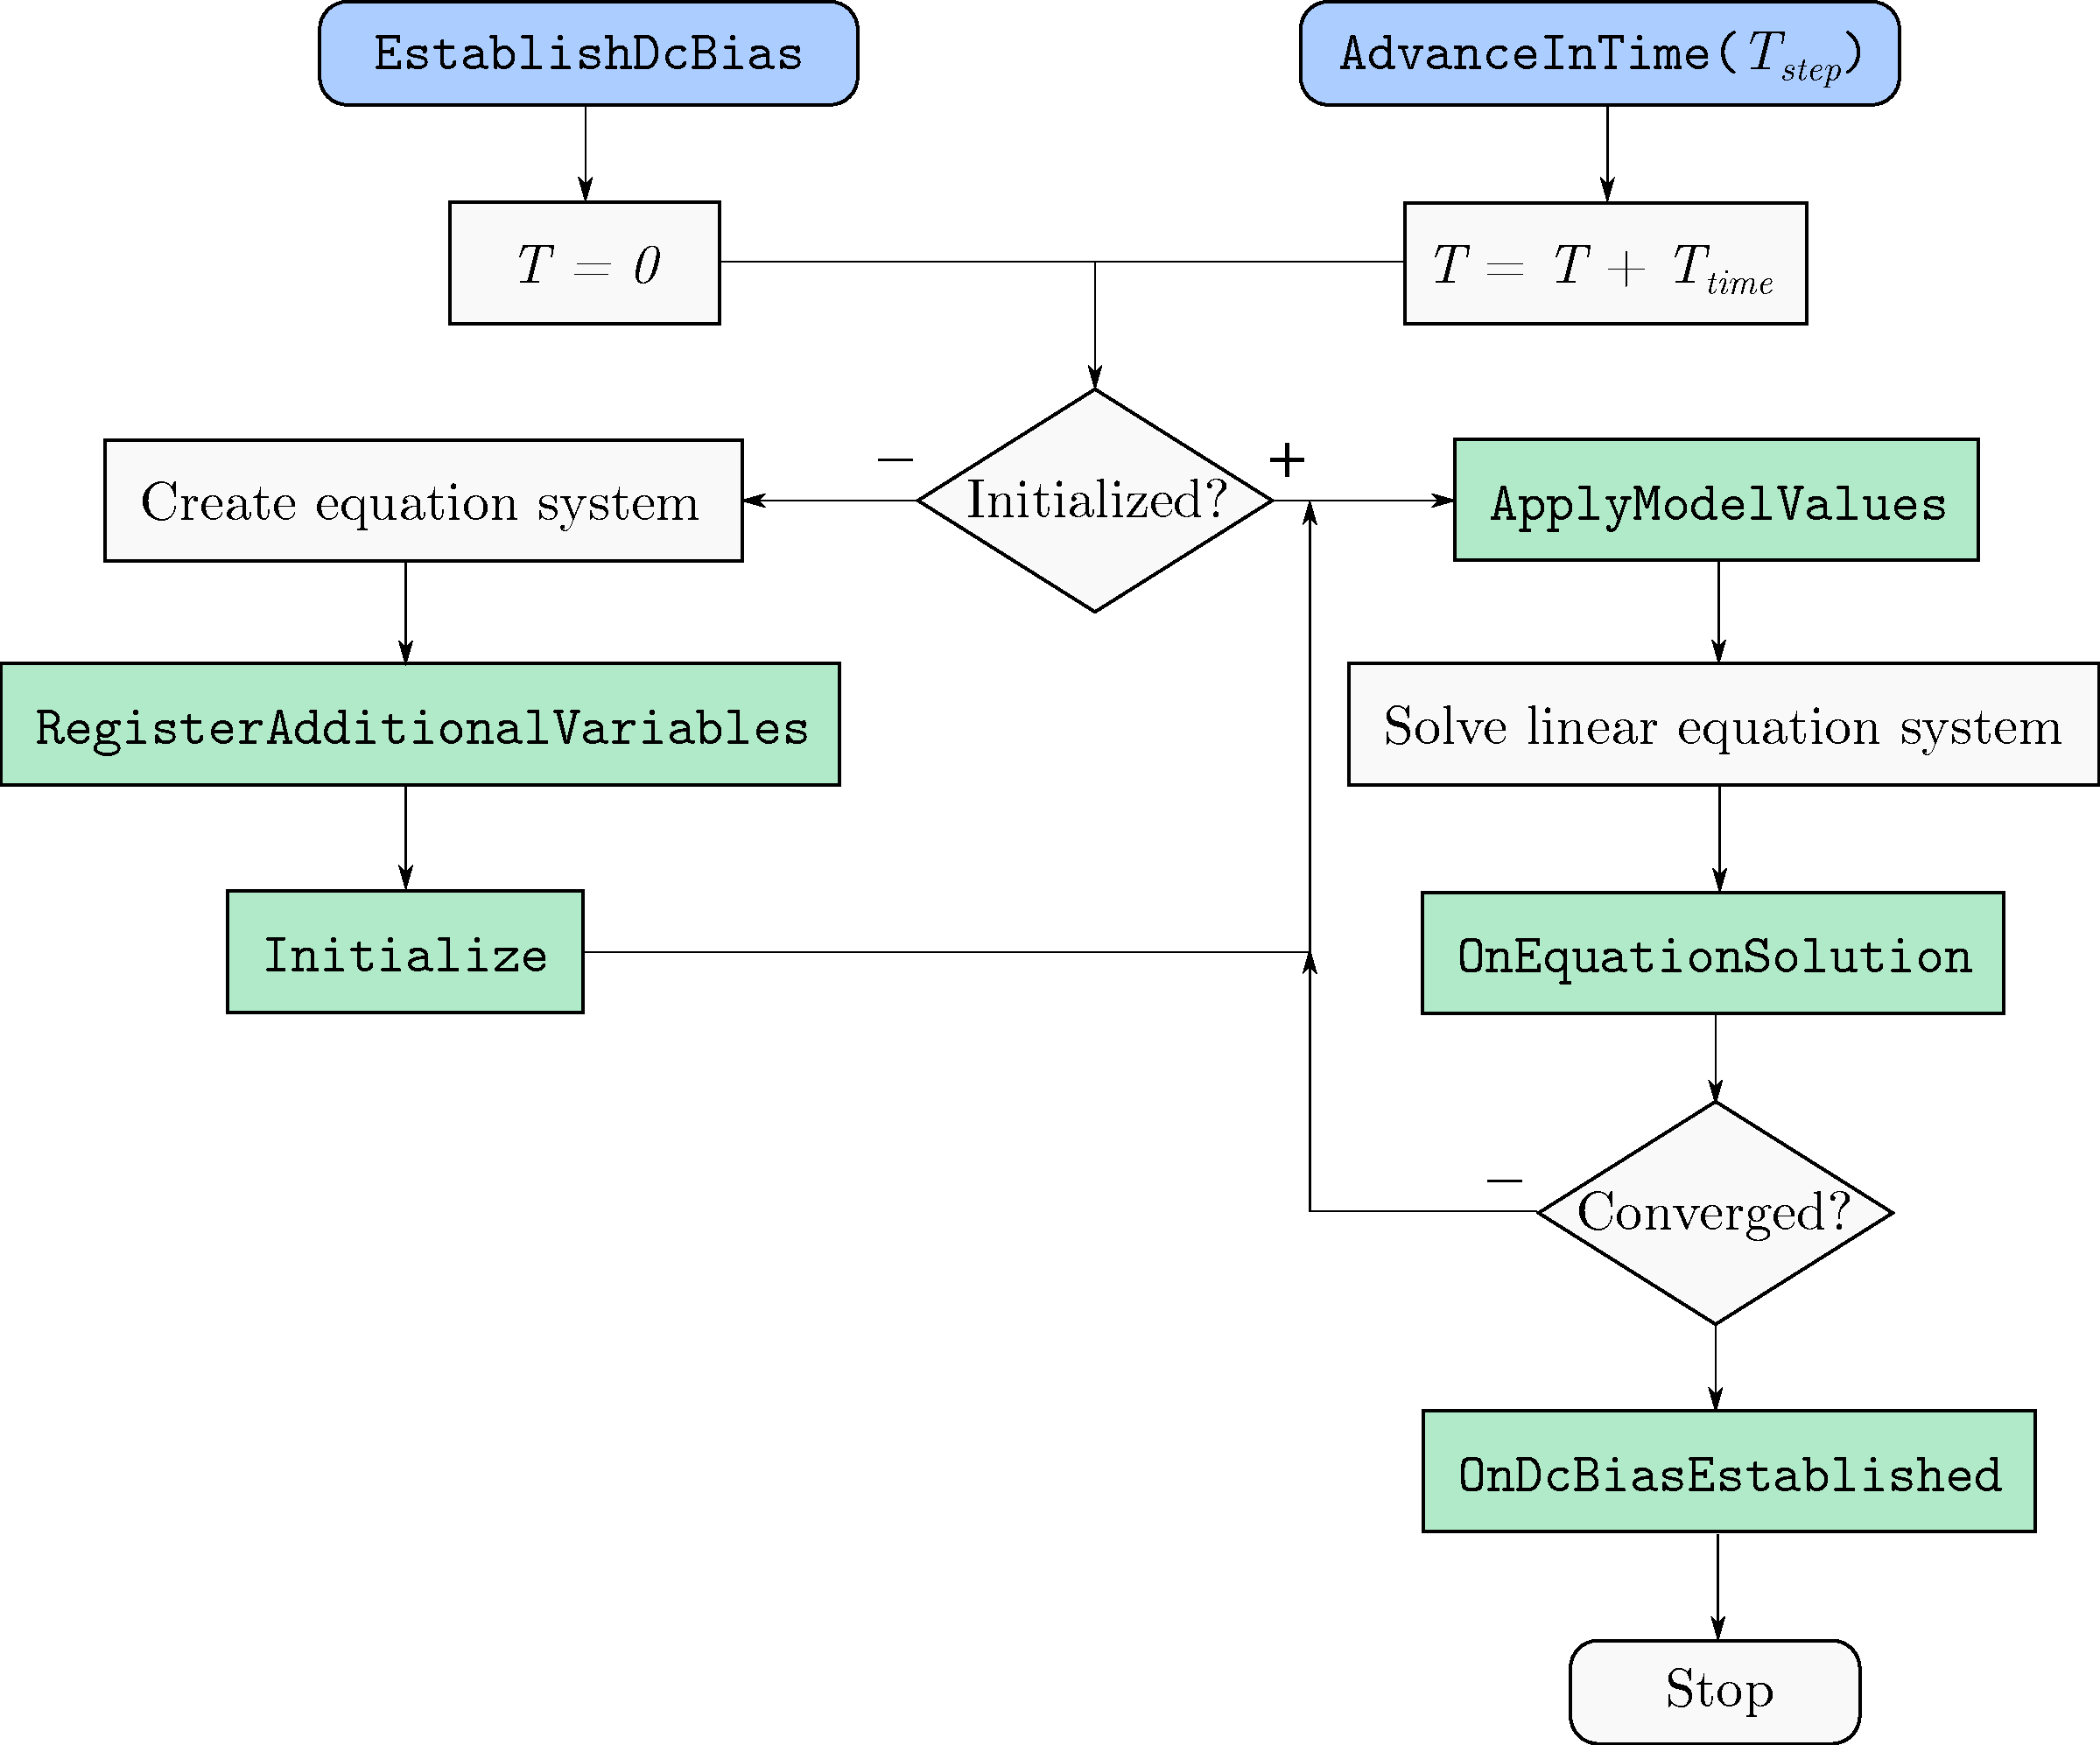
\includegraphics[width=\linewidth]{transient-analysis-implementation-diagram}
	\caption{Implementation of the simulation algorithm}
	\label{fig:transient-analysis-implementation-diagram}
\end{figure}

The following table lists the classes which implement the large-signal logic for individual circuit devices, and the corresponding section in QUCS Technical papers which describes the stamps and mathematical models used in the implementation. Also, the models for semiconductor devices (diode and BJT) are described in depth in Semiconductor Device Modeling with SPICE by G. Massobrio \cite{device_modeling}, ch 1 and 2.

\begin{center}
	\begin{tabular}{|l|l|}
		\hline
		Device class & QUCS section \\ \hline \hline
		\texttt{LargeSignalResistor} & 9.2 \\ \hline
		\texttt{LargeSignalCapacitor} & 6.3.1 \\ \hline
		\texttt{LargeSignalInductor} & 6.3.2 \\ \hline
		\texttt{LargeSignalVoltageSource} & 9.18 \\ \hline
		\texttt{LargeSignalCurrentSource} & 9.18 \\ \hline
		\texttt{LargeSignalVccs} & 9.20.1 \\ \hline
		\texttt{LargeSignalCccs} & 9.20.2 \\ \hline
		\texttt{LargeSignalVcvs} & 9.20.3 \\ \hline
		\texttt{LargeSignalCcvs} & 9.20.4 \\ \hline
		\texttt{LargeSignalDiode} & 10.2 \\ \hline
		\texttt{LargeSignalBjt} & 10.4 \\ \hline
	\end{tabular}
\end{center}

The actual stamping is delegated to \texttt{<device>Stamper} classes to make the implementation cleaner. 

\section[NextGenSpice.Numerics and NextGenSpice.Numerics.Native]{NextGenSpice.Numerics and \\ NextGenSpice.Numerics.Native}

\texttt{NextGenSpice.Numerics.Native} is the only C++ project in the solution. It is used to build a dynamically linked library, which contains the implementation of QD library used by NextGen SPICE for the double-double and quad-double precision types. It also contains a native implementation of the Gaussian elimination algorithm for solving the equation system to speed up the the simulation (see analysis section~\ref{chap:analysis:dd}).

\texttt{NextGenSpice.Numerics} is the managed counterpart of the \texttt{NextGenSpice\+.Numerics.Native} project. It contains C\# wrappers around the \texttt{dd\_real} and \texttt{qd\_real} types from QD library, with PInvoke calls to its exported methods. It also contains the managed implementation of Gaussian-elimination that is used when the library is compiled without the conditional compilation symbols mentioned at the beginning of this chapter.

\subsection{Equation System Implementation}
The \texttt{NextGenSpice.Numerics} project contains implementations of the equation system. There is a separate class for the equation system for each precision type: \texttt{EquationSystem}, \texttt{DdEquationSystem} and \texttt{QdEquationSystem}. These classes represent an equation system as a full matrix and vectors. To make the interface independent of the implementation and the actual precision type used, the equation system is exposed through the implementations of \texttt{IEquationSystem\+Adapter} and \texttt{IEquationSystemAdapterWide} interfaces. The first interface defines methods for getting proxies for individual equation system coefficients and the equation solution as described in the analysis chapter in section~\ref{chap:analysis:equation}. This interface will be exposed to the device's implementation. The other interface defines other methods that the simulator needs, like \texttt{Solve} and \texttt{Clear}. The actual implementation of these interfaces is requested from the static class \texttt{EquationSystemAdapterFactory}. This arrangement was chosen mainly to allow runtime changes of precision type for benchmarking purposes.

If the implementation were to change to a sparse matrix representation, then all that needs to be done is implementing the \texttt{IEquatioSystemAdapterWide} interface and replacing the class instantiated in the \texttt{EquationSystemAdapterFactory}.

\section{NextGenSpice}
This project contains the implementation of the standalone SPICE-like console application. This application directly uses the other parts of the NextGen SPICE library described in the preceding sections. This project implements necessary statement processors to handle \texttt{.PRINT}, \texttt{.OP} and \texttt{.TRAN} statements in the input netlist files. These statements are inserted into the \texttt{OtherStatements} collection on the \texttt{ParsingContext} and later retrieved from the property of same name on the \texttt{SpiceNetlistParserResult} object. If no error occurs while parsing the netlist, the application executes the requested simulations and prints the results on standard output.

\section{SandboxRunner}
This project serves only development purposes and is not deployed as part of the library. This project uses the BenchmarkDotNet NuGet package to run benchmarks for comparing the individual precision methods. It also contains examples of code which uses the library.

\section{Unit Test Projects}
There are three unit test projects in the solution, \texttt{NextGenSpice.Core.Test} for the core simulation library, \texttt{NextGenSpice.Parser.Test} for the parser and \texttt{NextGenSpice.LargeSignal.Test} for the large-signal simulations. These project use the XUnit NuGet package to run unit tests for the main parts of the tested projects. The unit tests do not aim for strict 100\% code coverage (The coverage is around 80\% for each project), instead, they test the most important parts of the library to avoid breaking the code when implementing new features in the library.

\chapter{User Documentation - Library}

This chapter describes how to use the NextGen SPICE simulator, and provides the guidelines for adding new circuit analyses and device types. The necessary binaries are available in the \texttt{/binaries} folder on the attached CD for copying. 

\section{Tutorials}
This sections shows the usage of the library on simple examples to present the basic idea of how to use the NextGen SPICE library. All these examples will use the .NET Core Console Application project template. The project should reference the \texttt{NextGenSpice.Core} assembly for circuit description, \texttt{NextGenSpice.Parser} assembly for parser implementation, \texttt{NextGenSpice.LargeSignal} assembly for the actual simulator, and all assemblies with the \texttt{System.Composition} preffix from the \texttt{/binaries} folder. Also, \texttt{NextGenSpice.Numerics.Native.dll} needs to be copied to the same folder as the compiled executable. We will use gnuplot \cite{gnuplot} to create the plots of the simulation results, so reader should have it installed as well.

\subsection{Calculating DC Bias of the Ciruit}
Suppose we wanted to calculate node voltages in the circuit shown in figure \ref{fig:userdocs:simple-circuit}.

\begin{figure}[h]
	\centering
	\begin{circuitdev}
		(0,0) 
		to[V=12<\volt>,invert] (3,0) node[label={-90:$1$}]{}
		-- (6,0)
		to[R, l=5<\ohm>, .-*] (6,3) node[label={3:$3$}]{}
		to[R, l=5<\ohm>] (3,3) node[label={$2$}]{}
		to[R, l=10<\ohm>] (0,3)
		-- (0,0)
	
		(3,0) to[R, l=10<\ohm>, *-*] (3,3)
		(0,1.5) -- (-0.5,1.5) node[ground]{}
	\end{circuitdev}
	\caption{Example circuit}
	\label{fig:userdocs:simple-circuit}
\end{figure}

Before we start with the actual analysis, we first need to construct the circuit representation. This is done using the \texttt{CircuitBuilder} class. Following code fragment constructs the circuit description of our circuit.

\begin{csharpcode}
// requires NextGenSpice.Core.Circuit and
// NextGenSpice.Core.Devices namespace
var builder = new CircuitBuilder();
builder
	.AddDevice(new[] {1, 0}, new VoltageSource(12))
	.AddDevice(new[] {0, 2}, new Resistor(10))
	.AddDevice(new[] {1, 2}, new Resistor(10))
	.AddDevice(new[] {2, 3}, new Resistor(5))
	.AddDevice(new[] {1, 3}, new Resistor(5));
var circuit = builder.BuildCircuit();
\end{csharpcode}

For convenience, class \texttt{CircuitBuilderExtensions} defines extensions methods that can be used to make the code more readable. The circuit can be equivalently created by the following code.

\begin{csharpcode}
// extensinos are contained in 
// NextGenSpice.Core.Extensions namespace
var builder = new CircuitBuilder();
builder
	.AddVoltageSource(1, 0, 12)
	.AddResistor(0, 2, 10)
	.AddResistor(1, 2, 10)
	.AddResistor(2, 3, 5)
	.AddResistor(1, 3, 5);
var circuit = builder.BuildCircuit();
\end{csharpcode}

The \texttt{circuit} object created in the preceding code fragments is only a description of the circuit. In the next step, we use it to create it's large-signal model, which we will use to perform the actual analysis.

\begin{csharpcode}
// requires NextGenSpice.LargeSignal namespace
// equivalent to
// var m = AnalysisModelCreator
//     .Instance.Create<LargeSignalCircuitModel>(circuit);
var model = circuit.GetLargeSignalModel();
\end{csharpcode}

The call to the method \texttt{EstablishDcBias} performs the actual node voltage calculation. Calculated node voltages can be found in an array in \texttt{LargeSignal\+CircuitModel.NodeVoltages} property.

\begin{csharpcode}
model.EstablishDcBias();
Console.WriteLine(model.NodeVoltages[1]); // 12 
Console.WriteLine(model.NodeVoltages[2]); //  8 
Console.WriteLine(model.NodeVoltages[3]); // 10 
\end{csharpcode}

The simulator also automatically calculates data for individual devices, and stores them in their large-signal model instances contained in the \texttt{LargeSignal\+CircuitModel.Devices} collection. In our case, all currents flowing through the circuit devices are calculated. As an example, we show how to get value of current flowing through the voltage source in our circuit. 

First, we need to identify the device in the collection. This can be done by providing a \textit{tag} parameter during the circuit representation construction. Arbitrary object can be used as a tag, we will use a string tag.

\begin{csharpcode}
builder
	.AddVoltageSource(1, 0, 12, "VS")
//	equivalent to
//  .AddDevice(new[] { 1, 0 }, new VoltageSourceDevice(12, "VS"))
	...
\end{csharpcode}

This tag is then used to query the \texttt{LargeSignalCircuitModel.Devices} collection, which stores the implementations of \texttt{ILargeSignalDevice} interface for each circuit from the description. For convenience, each analysis model defines method \texttt{FindDevice()} to simplify the syntax.

\begin{csharpcode}
// requires NextGenSpice.LargeSignal.Devices namespace
// equivalent to
// var vsource = (ITwoTerminalLargeSignalDevice) model.Devices
//	.SingleOrDefault(dev => Equals(dev.DefinitionDevice.Tag, "VS"));
var vsouce = (ITwoTerminalLargeSignalDevice) model.FindDevice("VS");
Console.WriteLine(vsouce.Current); // -0.8
\end{csharpcode}

The casting to \texttt{ITwoTerminalLargeSignalDevice} interface is necessary, because some circuit devices may have more than two terminals (e.g. transistors), and the Current property would note make sense for them. The whole example example then reads as follows:

\begin{csharpcode}
var builder = new CircuitBuilder();
builder
.AddVoltageSource(1, 0, 12, "VS")
.AddResistor(0, 2, 10)
.AddResistor(1, 2, 10)
.AddResistor(2, 3, 5)
.AddResistor(1, 3, 5);
var circuit = builder.BuildCircuit();

var model = circuit.GetLargeSignalModel(); ;
model.EstablishDcBias();

Console.WriteLine(model.NodeVoltages[1]); // 12
Console.WriteLine(model.NodeVoltages[2]); //  8
Console.WriteLine(model.NodeVoltages[3]); // 10

var vsouce = (ITwoTerminalLargeSignalDevice) model.FindDevice("VS");
Console.WriteLine(vsouce.Current); // -0.8
\end{csharpcode}

\subsection{Performing Transient Analysis}
\label{chap:tutorial-transient}
In previous section, we showed how to use the library to compute DC Bias of the circuit. Now we will show how to perform transient analysis. Consider the circuit shown in figure \ref{fig:userdocs:rlc-circuit}.

\begin{figure}[h]
	\centering
	\begin{circuitdev}
		(0,0) node[ground]{}
		to[V=5<\volt>, -*, invert] (0, 3) node[label=135:1]{}
		to[R=50<\ohm>] (3, 3) node[label=3:2]{}
		to[L=0.125<\henry>, *-*] (3, 0) node[label=305:3]{}
		to[C=1<\micro\farad>] (0, 0)
	\end{circuitdev}
	\caption{Simple series RLC circuit.}
	\label{fig:userdocs:rlc-circuit}
\end{figure}

We will calculate how the circuit behaves if the 5 V from the voltage source come in a sudden pulse. The NextGen SPICE library supports many input source behaviors, the full list can be found in section \ref{chap:devdocs:devices}. We will specify the desired behavior by passing an instance of \texttt{PulseBehavior} to voltage source when building the circuit. 

\begin{csharpcode}
var circuit = new CircuitBuilder()
	// behaviors are located in NextGenSpice.Core.BehaviorParams namespace
	.AddVoltageSource(1, 0, new PulseBehavior()
	{
		InitialLevel = 0,
		PulseLevel = 5,
		Delay = 5e-3, // 5 ms
		PulseWidth = 25e-3 // 25 ms
	})
	.AddResistor(1, 2, 50)
	.AddInductor(2, 3, 0.125)
	.AddCapacitor(3, 0, 1e-6)
	.BuildCircuit();
\end{csharpcode}

Then, as in the previous example, we get the \texttt{LargeSignalCircuitModel} and calculate the initial state of the circuit using the \texttt{EstablishDcBias()} method. After that, we can call the \texttt{AdvanceInTime()} method to perform the timesteps. Following code fragment can be then used to print voltage values of nodes 1 and 3 over time.

\begin{csharpcode}
var model = circuit.GetLargeSignalModel();
model.EstablishDcBias();

Console.WriteLine("Time V(1) V(3)");

var timestep = 0.2e-3; // use 0.2 ms timestep
while (model.CurrentTimePoint <= 55e-3) // simulate for 55 ms
{
	var time = model.CurrentTimePoint;
	var v1 = model.NodeVoltages[1];
	var v3 = model.NodeVoltages[3];
	
	Console.WriteLine($"{time} {v1} {v3}");
	
	model.AdvanceInTime(timestep);
}
\end{csharpcode}

If we redirect the program output to a file named \texttt{output.txt}, we can run gnuplot and use following commands to create a \texttt{plot.svg} file with plot of the voltage values over time as shown in figure \ref{fig:userdocs:rlc-plot}.

\begin{minted}[linenos, tabsize=4, fontsize=\footnotesize]{gnuplot}
set terminal svg size 600, 250
set output 'plot.svg'
set key autotitle columnhead
set xlabel 'Time'
set ylabel 'Value'
set grid ytics lt 0 lw 1 lc rgb '#bbbbbb'
set grid xtics lt 0 lw 1 lc rgb '#bbbbbb'
plot for [i=2:3] 'output.txt' using 1:i with lines
\end{minted}


\begin{figure}[h]
	\centering
	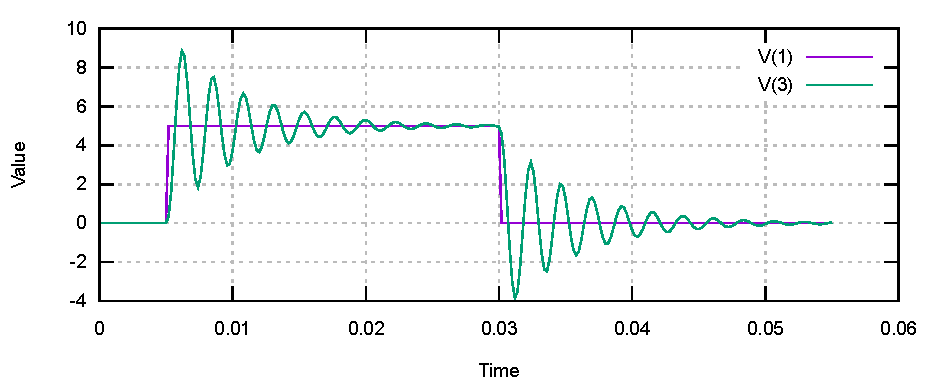
\includegraphics[width=0.8\linewidth]{04-fig-rlc-plot}
	\caption{Results on the RLC circuit.}
	\label{fig:userdocs:rlc-plot}
\end{figure}

\subsection{Loading Circuits from Netlists}

The NextGen SPICE library supports loading circuit description from SPICE netlist files. The supported syntax is shown in chapter \ref{chap:spicecode}. We will demonstrate this on the circuit shown in figure \ref{fig:back-to-back-circuit}. This is the same circuit we have shown earlier in the introduction chapter because of it's $1\mu\Omega$ resistor.

\begin{figure}[h]
	\begin{subfigure}{0.44\linewidth}
		\begin{spicecode}
Back to Back diodes
*
V1 IN 0 SIN(0 5 100 0 0 0)
D1 IN A D1N4148
R1 A B 1e-6
D2 0 B D1N4148
*
.MODEL D1N4148 D (
+ IS=2.52e-9 N=1.752 TT=2e-8
+ CJO=9e-13 M=0.25 VJ=20 BV=75
+ RS=0.568)
		\end{spicecode}
	\end{subfigure}
	\begin{subfigure}{0.55\linewidth}
	
		\centering
		\begin{circuitdev}
			(0,0) node[ground]{} -- (-2,0)
			to[sV<=5<\volt>,a=\text{V1 100Hz}] (-2,6) -- (0,6) node[circ,label=IN]{} -- (2,6)
			to[D,a=D1, l=D1N4148] (2,4) node[label=1:A]{} to[R=1<\micro\ohm>, a=R1, *-*] (2,2) node[label=1:B]{} to[D,invert, a=D2, l=D1N4148] (2,0) -- (0,0)
		\end{circuitdev}
	\end{subfigure}
	\caption{Back to back diode circuit and corresponding netlist}
	\label{fig:back-to-back-circuit}
\end{figure}

When imported from a netlist file, each device is automatically tagged by its name in uppercase letters so that it can be found among the other devices. Following code fragments prints the current flowing through the \texttt{D1} diode, and figure \ref{fig:04-fig-back-to-back-gear} shows the plot of the data.

\begin{csharpcode}
// parser is located in NextGenSpice.Parser namespace

// import circuit definiton from the file
var parser = SpiceNetlistParser.WithDefaults();
var result = parser.Parse(new StreamReader("circuit.cir"));
var circuit = result.CircuitDefinition;

// get simulation model
var model = circuit.GetLargeSignalModel();
var d1 = (ITwoTerminalLargeSignalDevice) model.FindDevice("D1");
var inNode = result.NodeIndices["IN"];

Console.WriteLine("Time V(IN) I(D1)");

var timestep = 10e-6; // use 10 us timestep
while (model.CurrentTimePoint <= 10e-3) // simulate for 10 ms
{
	var time = model.CurrentTimePoint;
	var vin = model.NodeVoltages[inNode];
	var id1 = d1.Current;
	
	Console.WriteLine($"{time} {vin} {id1}");
	
	model.AdvanceInTime(timestep);
}
\end{csharpcode}

\begin{figure}[h]
	\centering
	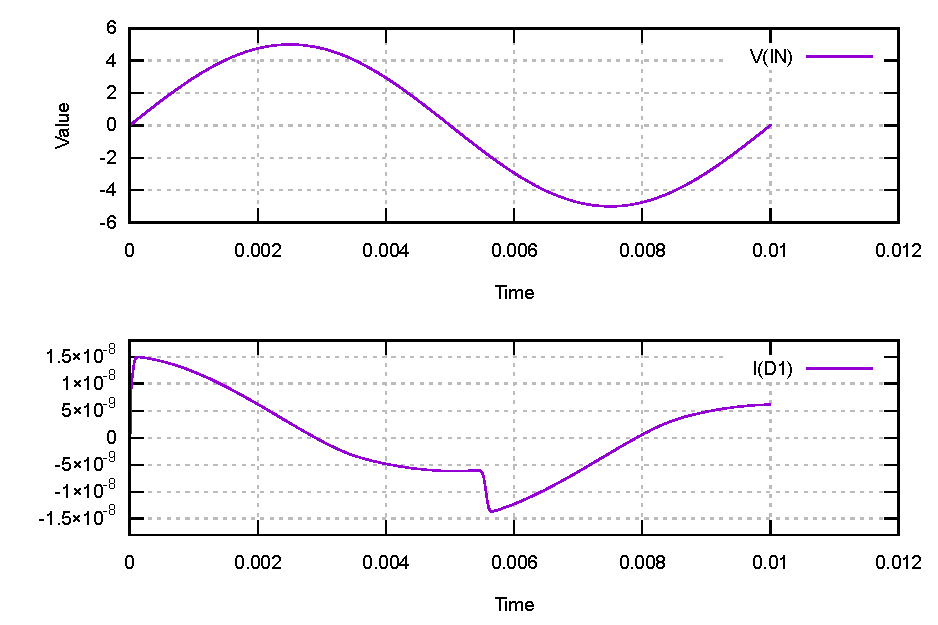
\includegraphics[width=.85\linewidth]{04-fig-back-to-back-gear}
	\caption{Plot of simulation output of back-to-back diode circuit.}
	\label{fig:04-fig-back-to-back-gear}
\end{figure}

\subsection{Defining a Subcircuit in Source Code}

NextGen SPICE support defining a custom subcircuit, which then can be used multiple times throughout the circuit and even in different circuits. In this tutorial, we will define a subcircuit representing a $9V$ battery with $1.5\Omega$ internal resistance, which is modelled as $9V$ voltage source and $1.5\Omega$ resistor in series, as shown in figure \ref{fig:userdocs:battery}.

\begin{figure}[h]
	\begin{circuitdev}
		(0,0) node[circ,label=N-]{} to[V=9<\volt>, invert] (3,0) to[R=1.5<\ohm>] (6,0) node[circ,label=N+]{}
	\end{circuitdev}
	\caption{Subcircuit for $9V$, $1.5\Omega$ battery}
	\label{fig:userdocs:battery}
\end{figure}

The subcircuit is created using the \texttt{CircuitBuilder} class, just as if it were a normal circuit, only instead of \texttt{BuildCircuit()} method, the \texttt{BuildSubcircuit()} method needs to be called with an array specifying which subcircuit nodes should be treated as terminals. The battery definition then can be used as an argument to \texttt{AddSubcircuit()} extension method, or passed to the \texttt{SubcircuitDevice} class constructor. Following code fragment constructs part of a circuit with two $9V$ batteries in series.

\begin{csharpcode}
var builder = new CircuitBuilder();
var batteryDefinition = builder
	.AddVoltageSource(1, 2, 9)
	.AddResistor(2, 3, 1.5)
	.BuildSubcircuit(new [] {1, 3});

builder.Clear();
builder
	.AddDevice(new[] {0, 1}, new Subcircuit(batteryDefinition))
	.AddSubcircuit(new[] {1, 2}, batteryDefinition);
	...
\end{csharpcode}


It is also possible to inspect the state of the devices inside the subcircuit during simulation. The \texttt{SubcircuitDevice}'s counterpart in \texttt{LargeSignalDeviceModel\+.Devices} implements \texttt{ILargeSignalSubcircuit} interface, which exposes the devices inside via the \texttt{Devices} property.

In this section, we described the usage of the simulator on simple examples, in next section, we revisit individual parts of the simulator and provide detailed description of it's interface.

\section{NextGenSpice.Core}

The \texttt{NextGenSpice.Core} assembly contains the analysis independent parts of the NextGen SPICE library, namely the classes for circuit description, and logic for validating the circuit.

\subsection{Creating the Circuit Description}
As we briefly described in the tutorials in previous section. The NextGen SPICE library works by first creating an analysis-independent \texttt{CircuitDefinition} class, which is then transformed into the analysis-dependent circuit model. The description of the circuit (the \texttt{CircuitDefinition} class) is created using the \texttt{Circuit\+Builder} class using the \texttt{Add(int[] terminals, ICircuitDefinitionDevice device)} method. The circuit builder then saves the reference to the device and sets node connections appropriately. If multiple copies of the same device should be added to the circuit, it is necessary to clone the device via the \texttt{ICircuitDefinitionDevice.Clone} method.

For convenience, there is a static class \texttt{CircuitBuilderExtensions} which contains extension methods on \texttt{CircuitBuilder} like \texttt{AddResistor}, \texttt{AddDiode} etc., which can be used to shorten the code that adds the individual devices.

\subsection{Supported Circuit Devices}
\label{chap:devdocs:devices}
Following table lists devices available in the NextGen SPICE simulation library. 

\begin{center}
	\begin{tabular}{|l|l|l|}
		\hline
		Device & Nodes & Parameters \\ \hline \hline
		\texttt{Resistor} & $N_+$, $N_-$ & Resistance \\ \hline
		\texttt{Capacitor} & $N_+$, $N_-$ & Capacitance, initial voltage \\ \hline
		\texttt{Inductor} & $N_+$, $N_-$ & Inductance, initial current \\ \hline
		\texttt{VoltageSource} & $N_+$, $N_-$ & Voltage or \texttt{InputSourceBehavior} \\ \hline
		\texttt{CurrentSource} & $N_+$, $N_-$ & Current or \texttt{InputSourceBehavior} \\ \hline
		\texttt{Vccs} & $N_+$, $N_-$, $N_{Ref+}$, $N_{Ref-}$ & Gain \\ \hline
		\texttt{Vcvs} & $N_+$, $N_-$, $N_{Ref+}$, $N_{Ref-}$ & Gain \\ \hline
		\texttt{Cccs} & $N_+$, $N_-$ & \texttt{VoltageSource}, gain \\ \hline
		\texttt{Ccvs} & $N_+$, $N_-$ & \texttt{VoltageSource}, gain \\ \hline
		\texttt{Diode} & $N_+$, $N_-$ & \texttt{DiodeParam} \\ \hline
		\texttt{Bjt} & $N_{C}$, $N_{B}$, $N_{E}$, $N_{S}$ & \texttt{BjtParam} \\ \hline
	\end{tabular}
\end{center}

The parameters listed in the table are set in the class constructor and directly map to the SPICE netlist statement parameters which were described in depth in section \ref{chap:spicecode-devices}. The \texttt{DiodeParam} and \texttt{BjtParam} classes encapsulate the model parameters for the diode and BJT devices, and again map to the same parameters as in the netlist \texttt{.MODEL} parameters. Additionally, each device class accepts an optional \texttt{object} parameter as its tag.

The \texttt{InputSourceBehavior} class is the base class for several source behavior specification classes. Again, these classes directly map to the transient input sources from the SPICE netlist syntax, as described in \ref{chap:spicecode-input-sources}. The supported behaviors are listed in the following table.

\begin{center}
	\begin{tabular}{|l|l|l|}
		\hline
		Behavior class & Netlist & Description \\ \hline \hline
		\texttt{ConstantBehavior} & DC & Constant input source value \\ \hline
		\texttt{SinusoidalBehavior} & SIN & Sinusoidal source \\ \hline
		\texttt{PieceWiseLinearBehavior} & PWL & Arbitrary piece-wise linear source \\ \hline
		\texttt{PulseBehavior} & PULSE & Source with regular pulses  \\ \hline
		\texttt{ExponentialBehavior} & EXP & Source with exponential edges \\ \hline
		\texttt{AmBehavior} & AM & Amplitude modulated source \\ \hline
		\texttt{SffmBehavior} & SFFM & Single frequency modulated source \\ \hline
	\end{tabular}
\end{center}

\subsection{Creating Analysis-Specific Circuit Models}

Before any circuit analysis can be performed, the circuit definition must be transformed into the analysis-specific circuit model. NextGen SPICE currently supports only the \texttt{LargeSignalCircuitModel} which will be described in section \ref{chap:userdocs-large-signal} in more detail.

The circuit models are created using the \texttt{AnalysisModelCreator} class and its instance method \texttt{GetModel<TCircuitModel>(ICircuitDescription)}. This class encapsulates \texttt{IAnalysisModelFactory<TCircuitModel>} implementations for individual analysis model types. Factory implementations for analysis models provided by NextGen SPICE library are automatically registered using the MEF framework. These factories can be configured to use specific implementations for individual circuit devices. The configuration is done on the factory itself, which can be obtained using the \texttt{AnalysisModelCreator.GetFactory<TCircuit\+Model>()}.

There is a global instance of the \texttt{AnalysisModelCreator} class available at \texttt{AnalysisModelCreator.Instance} property. There is also an extension method on the \texttt{ICircuitDefinition} interface which uses the global model creator to create the \texttt{LargeSignalCircuitModel}, which can be used to simplify the code.

\section{NextGenSpice.Parser}
The NextGenSpice.Parser assembly contains the implementation of the SPICE netlist parser. The parser itself is represented by the \texttt{SpiceNetlistParser} class. The parser is designed to be extensible by registering statement processors for individual netlist statements, which will be covered later. An instance of the parser can be obtained via static methods \texttt{SpiceNetlistParser.Empty()} which return an instance of the parser without any statement processors registered, and \texttt{SpiceNetlistParser.WithDefaults()} which returns instance with handlers for all devices implemented in the NextGen SPICE library.

The parsing itself is done using the \texttt{Parse} method which returns an instance of \texttt{SpiceNetlistParserResult} which contains following properties:

\begin{itemize}
	\item \texttt{CircuitDefinition} -- Definition of the circuit contained in the netlist.
	\item \texttt{Subcircuits} -- Collection of \texttt{ISubcircuitDefinition} classes for the subcircuits defined in the top-level of the netlist (Subcircuits defined inside another subcircuit are not returned).
	\item \texttt{Models} -- collection of device model (parameter sets) defined in the netlist (again, models defined inside a subcircuit are not returned).
	\item \texttt{Title} -- The content of the title statement from the netlist.
	\item \texttt{Errors} -- Collection of \texttt{SpiceParserError} classes which wrap the errors encountered during the parsing.
	\item \texttt{NodeNames} -- NextGen SPICE uses \texttt{int} type to store the id of a node, this array can be indexed by the node id to obtain the string name that was used in the netlist. 
	\item \texttt{NodeIndices} -- Dictionary providing the inverse mapping to \texttt{NodeNames} property.
	\item \texttt{OtherStatements} -- Collection of \texttt{SpiceStatement}s that can be used to return user-defined statements from the parser.
\end{itemize}

To simplify obtaining references to individual circuit device instances, each instance has been tagged with the uppercase name of the device used in the netlist, so that a particular device can be easily obtained by \texttt{FindDevice} methods on circuit definition and circuit models.


\section{NextGenSpice.LargeSignal}
\label{chap:userdocs-large-signal}

The \texttt{NextGenSpice.LargeSignal} assembly contains the implementation of the large-signal circuit model which is used to perform transient analysis of circuits. The simulation functionality is exposed through the \texttt{LargeSignalCircuitModel} class, and its \texttt{EstalblishDcBias} and \texttt{AdvanceInTime} instance methods. The \texttt{EstablishDcBias} method is used to calculates the DC bias of the circuit at initial timepoint, and \texttt{AdvanceInTime} method is used to get the DC bias after given timestep.

\subsection{Accessing the Computed State}
The calculated node voltages are stored in an array in the \texttt{NodeVoltages} property on the \texttt{LargeSignalCircuitModel} class. The \texttt{Devices} property stores large-signal representation classes as \texttt{ILargeSignalDevice} instances for the devices used in the circuit. These instances can be used to inspect the state computed for each circuit device. The \texttt{ILargeSignalDevice} instance for a particular device can be obtained by using the \texttt{FindDevice} method, which has overloads accepting \texttt{ICircuitDefinitionDevice} instance, or an \texttt{object} which was used as a tag during circuit construction. The state is exposed in two ways: \texttt{GetDeviceState\+Providers} method returning a collection of \texttt{IDeviceStateProvider} classes, and through the individual properties on the device implementation instance.

The \texttt{IDeviceStateProvider} instances can be used to print all the available state variables. The \texttt{Name} property gives the name of the variable, like "I" for the current flowing through the device, and \texttt{GetValue} method can be used to obtain the respective value.

The same state can be accessed through individual properties on the device implementation class instance. For example, in case of two terminal devices like resistor or voltage source, the respective class implements the \texttt{ITwoTerminalLarge\+SignalDevice} interface, which exposes \texttt{Voltage} and \texttt{Current} property containing the voltage across the device and current flowing through the device, respectively. The \texttt{ITwoTerminalLargeSignalDevice} interface is implemented by all implemented devices except the BJT transistor.

The BJT transistor implementation class \texttt{LargeSignalBjt} exposes properties \texttt{CurrentBase}, \texttt{CurrentCollector} and \texttt{CurrentEmitter} which expose the currents flowing through the respective terminals, and \texttt{VoltageBaseCollector}, \texttt{VoltageBaseEmitter} and \texttt{VoltageCollector\+Emitter} for voltages between individual pairs of terminals.

\subsection{Modifying the Device Parameters}
The device's implementation used in the \texttt{LargeSigalCircuitModel} retain references to the corresponding circuit definition classes. This means that changes made to the device parameters inside \texttt{CircuitDefinition} are reflected in the next DC bias point calculation. To demonstrate, recall the circuit we used in the DC Bias calculation tutorial (figure \ref{fig:userdocs:simple-circuit}). The following code snippet prints the DC bias values for increasing values of the rightmost resistor.

\begin{csharpcode}
// build circuit	
var builder = new CircuitBuilder();
builder
	.AddVoltageSource(1, 0, 12, "VS")
	.AddResistor(0, 2, 10)
	.AddResistor(1, 2, 10)
	.AddResistor(2, 3, 5)
	.AddResistor(1, 3, 5, "R1");
var circuit = builder.BuildCircuit();
var model = circuit.GetLargeSignalModel();
var vsouce = (ITwoTerminalLargeSignalDevice)model.FindDevice("VS");
var res = (ResistorDevice)circuit.FindDevice("R1");

// sweep for values from 1 Ohm to 15 Ohm
for (int i = 1; i <= 15; i++)
{
	res.Resistance = i+1; // set resistance
	
	// calculate
	model.EstablishDcBias();
	var v1 = model.NodeVoltages[1];
	var v2 = model.NodeVoltages[2];
	var v3 = model.NodeVoltages[3];
	var iV = vsouce.Current;
	
	// print values
	Console.WriteLine($"{i+1}Ohm: {v1}V {v2}V {v3}V {iV}A");
}
\end{csharpcode}

\subsection{Changing the Integration Method}
Some circuits are sensitive to the choice of numerical integration method used during the simulator. The default integration method is GEAR-2 method, which is a reasonable compromise between accuracy and stability. However, use of GEAR-2 method dampens the oscilations of RLC circuits. Consider the trivial circuit in figure \ref{fig:oscillation-circuit}. Because this circuit lacks any resistance, the voltage at node 1 should oscillate indefinitely with amplitude of 1V.

\begin{figure}[h]
	\centering
	\begin{circuitdev}
		(0,0) node[circ,label=1]{} -- (-1,0) to[C, a=1<\nano\farad>] (-1,-3) -- (0,-3) node[ground]{} -- (1,-3)  to[L, a=1<\micro\henry>,i_=\mbox{$i=1mA$}] (1,0) -- (0,0)
	\end{circuitdev}
	\caption{Indefinitely oscillating circuit}
	\label{fig:oscillation-circuit}
\end{figure}

However, the GEAR-2 method dampens the oscillation. The simulator results with GEAR-2 method are shown in figure \ref{fig:oscillation-gear}

\begin{figure}[H]
	\centering
	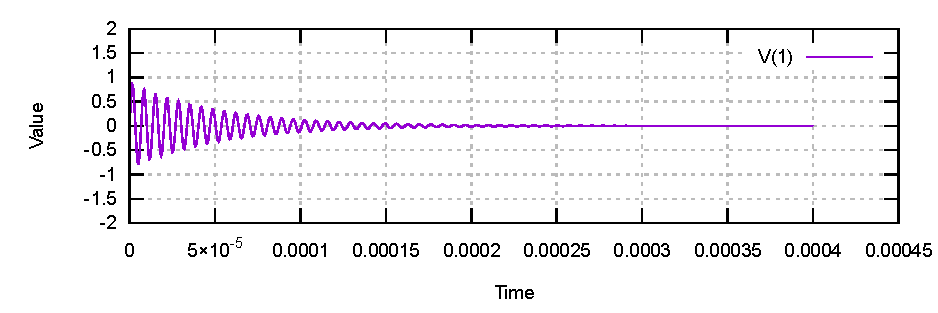
\includegraphics[width=.85\linewidth]{oscillation-gear}
	\caption{Simulation results on oscillating circuit using GEAR-2 method}
	\label{fig:oscillation-gear}
\end{figure}

For comparison, the figure \ref{fig:oscillation-trap} shows the same simulation with trapezoidal integration method.

\begin{figure}[h]
	\centering
	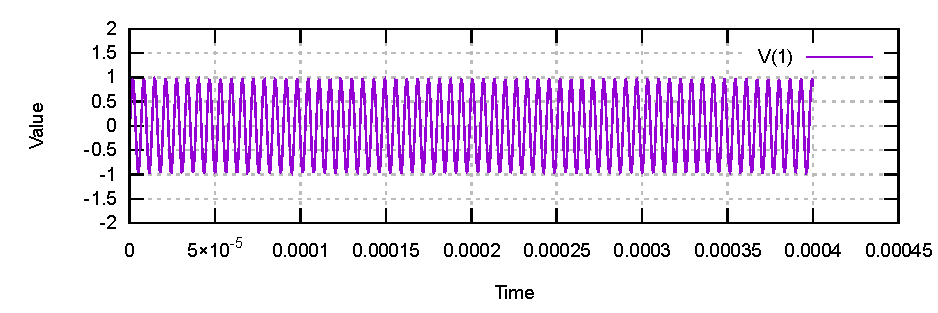
\includegraphics[width=.85\linewidth]{oscillation-trap}
	\caption{Simulation results on oscillating circuit using trapezoidal rule}
	\label{fig:oscillation-trap}
\end{figure}

Even though the trapezoidal method is more precise in terms of smaller local truncation error and does not dampen the oscillations, it is less stable than other methods. For comparison figure \ref{fig:04-fig-back-to-back-trap} shows plots of data obtained using the trapezoidal rule on the back-to-back diode circuit we have shown back in figure \ref{fig:back-to-back-circuit}. Notice the numerical noise, also known as \textit{trapezoidal ringing}, present in the plot.\footnote{We have increased the timestep to $100\mu{}s$, the original $10\mu{}s$ timestep also produces numerical oscilation, but due to the density of the oscilation the plot would be merged into a single thick line.}

\begin{figure}[h]
	\centering
	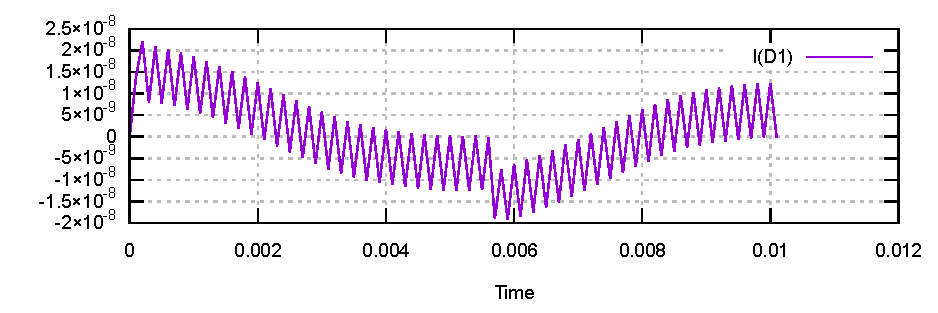
\includegraphics[width=.85\linewidth]{04-fig-back-to-back-trap}
	\caption{Simulation results of back-to-back diode using the trapezoidal rule}
	\label{fig:04-fig-back-to-back-trap}
\end{figure}

The numerical method that is used during the simulation can be changed by replacing the \texttt{IntegrationMethodFactory} property on \texttt{LargeSignalCircuit\+Model.CircuitParameters} object. Following code fragment shows how to configure the simulator to use the Trapezoidal Rule integration method.

\begin{csharpcode}
LargeSignalCircuitModel model = /* ... */;

// requires NextGenSpice.LargeSignal.NumIntegration namespace
model.CircuitParameters.IntegrationMethodFactory =
	new SimpleIntegrationMethodFactory(
		() => new TrapezoidalIntegrationMethod());
\end{csharpcode}

The supported integration methods are listed in the following table

\begin{center}
	\begin{tabular}{|l|l|}
		\hline
		Integration method & Class name \\ \hline \hline
		GEAR method & \texttt{GearIntegrationMethod} \\ \hline
		Trapezoidal rule & \texttt{TrapezoidalIntegrationMethod} \\ \hline
		Backward (implicit) Euler & \texttt{BackwardEulerIntegrationMethod} \\ \hline
		Adams Moulton & \texttt{AdamsMoultonIntegrationMethod} \\ \hline
	\end{tabular}
\end{center}

\chapter{Extending the Library}
\label{chap:exteding}
This chapter describes the functionality of the library can be extended by the user. Also, in section \ref{chap:userdocs:diode-tutorial}, we provide an example code that implements a simple diode device that will demonstrate the process on a concrete example.

\section{Adding New Circuit Devices}
Adding new circuit devices requires both creating a class that is used in circuit description and class that implements the actual large-signal simulation logic. We will describe both parts in separate subsections.

\subsection{Adding Device Description}

Each device description class must implement the \texttt{ICircuitDefinitionDevice} interface. To simplify the implementation of new devices, the library provides basic implementation of this interface in \texttt{CircuitDefinitionDevice} abstract class. Furthermore, there exists \texttt{TwoTerminalCircuitDevice} abstract class which defines additional member which can be useful for devices with two terminals. 

These classes can be then immediately used as arguments to the \texttt{Circuit\+Builder.AddDevice} method and thereby in the circuit definition. If the device should participate in the circuit topology validation, then the derived classes should override the \texttt{GetBranchMetadata} method and return the \texttt{CircuitBranch\+Metadata} instances that describe which terminals are connected by voltage-defined and current-defined branches.

\subsection{Adding Large-Signal Device Implementation}

To use these devices during a circuit analysis, their analysis-specific logic must be implemented and then registered in the respective \texttt{IAnalysisModelFactory} instance, so that the \texttt{AnalysisModelCreator} knows which implementation to use when creating the \texttt{LargeSignalCircuitModel}.

The Device's large-signal implementation needs to implement the \texttt{ILarge\+SignalDevice} interface. This interface defines following members:

\begin{itemize}
	\item \texttt{RegisterAdditionalVariables} -- Allows implementation to add additional variables to the equation system via supplied \texttt{IEquationSystemAdapter} instance.
	\item \texttt{Initialize} -- Lets devices request equation system proxies from \texttt{IEquation\+SystemAdapter}, and perform other necessary initialization, like getting numerical integrators from \texttt{ISimulationContex.SimulationParameters.\+IntegrationMethodFactory}.
	\item \texttt{ApplyModelValues} -- Applies devices MNA stamp into the equation system. If the device is nonlinear, the linearized equivalent circuit should be stamped.
	\item \texttt{OnEquationSolution} -- Lets devices check for solution convergence (compare current solution with the previous one). The tolerancies can be accessed in \texttt{ISimulationContext.SimulationParameters} object, and if the solution did not converge, the \texttt{ISimulationContext.ReportNotConverged} method should be called.
	\item \texttt{OnDcBiasEstablished} -- Called after the Newton-Raphson iterations have reached a fixed point and the calculation of the current timestep has completed.
\end{itemize}

The mapping between circuit definition classes and their analysis implementations is done for each analysis model separately by calling the \texttt{SetModel<TRep, TMod>} method on the respective \texttt{IAnalysis\+ModelFactory} instance. The method accepts a function which creates the implementation class from the circuit definition class. The following code snippet shows how to register \texttt{LargeSignal\+Resistor} as the implementation of \texttt{Resistor} device for \texttt{LargeSignalCircuit\+Model}.

\begin{csharpcode}
var factory = AnalysisModelCreator.Instance
	.GetFactory<LargeSignalCircuitModel>();

factory.SetModel<Resistor, LargeSignalResistor>(
	resistor => new LargeSignalResistor(resistor));
\end{csharpcode}

This mapping can be later changed by another call to \texttt{SetModel} method. It is also possible to create separate \texttt{AnalysisModelCreator} instances and have different mappings in each instance.

\section{Extending the Parser}

An optional step when adding a new device to the simulator is extending the parser to allow importing the new device from spice netlists.

\subsection{Adding New Device Processors}

The parser implemented in NextGen SPICE library delegates parsing of individual device statements to classes implementing the \texttt{IDeviceStatementProcessor} interface. Implementations of this interface can be added to the parser by calling the \texttt{RegisterDevice} method. We recommend creating new device statement processors by deriving from \texttt{DeviceStatementProcessor} abstract class. The derived class then needs to implement only the \texttt{Discriminator} char property which specifies the letter identifying the device (The letter should be uppercase), and \texttt{DoProcess} method that does the actual processing.

For simple devices with no dependencies, the \texttt{DoProcess} method may directly add the device to the \texttt{CircuitBuilder} accessible on the \texttt{protected} property of the same name in \texttt{DeviceStatementProcessor}. In case of devices like diode which depend on other statements (diode statement depends on \texttt{.MODEL} statement which defines its model parameters), the statement processing needs to be deferred until later. This is done by adding a \texttt{DeferredStatement} on the active \texttt{ParsingContext} accessible through the \texttt{Context} property of \texttt{DeviceStatement\+Processor} base class. The \texttt{DeferredStatement} defines the following methods.

\begin{itemize}
	\item \texttt{CanApply} -- Should return \texttt{true} if all dependencies of the statement have been processed and the statement can be processed next.
	\item \texttt{Apply} -- Should add the device into the circuit using the \texttt{CircuitBuilder} on the \texttt{ParsingContext}
	\item \texttt{GetErrors} -- Should return a collection of \texttt{SpiceParserErrors} that describe errors prevent the statement processing. This method is called once it is certain that no statement can be processed.
\end{itemize}

The \texttt{DeviceStatementProcessor} class also provides property \texttt{DeviceName} that exposes the name of the currently parsed device, and following methods.

\begin{itemize}
	\item \texttt{GetNodeIds(int start, int count)} -- Returns node ids of \texttt{count} nodes specified in the statement starting by token on with index \texttt{start}.
	\item \texttt{GetValue(int index)} -- parses the numeric value out of the token on \texttt{index}th token.
\end{itemize}

Both these method do the necessary error handling. The number of errors generated can be checked in the \texttt{Errors} property, and additional errors can be added to the \texttt{Context.Errors} collection. If no error is encountered, the processor should either add the device to the circuit using the \texttt{CircuitBuilder} property, or add a \texttt{DeferredStatement} to \texttt{Context.DeferredStatements} collection. The following code fragment shows how the resistor statements are parsed.

\begin{csharpcode}
protected override void DoProcess()
{
	var nodes = GetNodeIds(1, 2);
	var rvalue = GetValue(3);
	
	if (Errors == 0)
		CircuitBuilder.AddDevice(nodes, new Resistor(rvalue, DeviceName));
}
\end{csharpcode}

Because the resistor device does not depend on any other statement, the device can be added to the circuit straight away. In case of diode statements, diode devices cannot be added to circuit until the corresponding \texttt{.MODEL} statement is parsed. Because \texttt{.MODEL} statements are used to set parameters for many device types, there is a \texttt{ModeledDevice\+DeferredStatement<T>} class deriving from \texttt{DeferredStatement}. which implements the checking for models. This class is used in the \texttt{DiodeStatementProcessor} as shown in the following code fragment.

\begin{csharpcode}
protected override void DoProcess()
{
	var nodes = GetNodeIds(1, 2);
	// cannot check for model existence yet, defer checking for model later
	
	if (Errors > 0)	return;
	
	var name = DeviceName; // captured in lambda
	var modelToken = RawStatement[3];
	Context.DeferredStatements.Add(
		new ModeledDeviceDeferedStatement<DiodeParams>(
			scope: Context.CurrentScope,
			addFunc: (par, cb) => cb.AddDevice(nodes, new Diode(par, name)),
			modelNameToken: modelToken));	
}
\end{csharpcode}

\subsection{Adding New Model Types}

Some devices (like diode and BJT transistor) require a corresponding \texttt{.MODEL} statement. The SpiceNetlistParser therefore can be extended to parse new models for new devices. The handling of models for the device is done by returning \texttt{IDeviceModelHandler} instances that do the parsing. The library again supplies a abstract class \texttt{DeviceModelHandlerBase<TParam>} that implements the basic logic. Derived classed need only specify the mapping to the parameter names. We show an example implementation of the \texttt{IDeviceModelHandler} later in section \ref{chap:userdocs:diode-example:parser}.

\section{Example: Adding a Diode Device}
\label{chap:userdocs:diode-tutorial}

In previous sections we described all the steps needed to add a new device to the simulator. To provide a concrete example, we will show in this section how to implement a simple diode device. The NextGen SPICE library already contains diode device implementation, represented by classes \texttt{Diode} and \texttt{LargeSignalDiode}, which is more complex version of the one we will show in this section. The library is designed so that circuit description classes can be reused, and the new diode implementation would require implementing only the device's large-signal logic. However, to demonstrate how completely new devices can be added to the library, we will not reuse the existing diode class. Our diode will be modeled solely by the Shockley diode equation and parameters shown in figure \ref{fig:userdocs:tutorial:diode-params}. The names in capital letters will be later used in diode statements in SPICE netlists. 

\begin{figure}[h]
	\centering
	
	\[ I = I_S \left(e^{\frac{V}{n \cdot V_t}} - 1 \right) \]
	
	\begin{tabular}{|l|l|l|}
		\hline 
		Parameter & Name & Description \\ \hline \hline
		$I_S$ & IS & Saturation current \\ \hline
		$n$ & N & Ideality coefficient \\ \hline
		$V_t$ & VT & Thermal voltage \\ \hline
		
	\end{tabular}
	
	\caption{Shockley diode equation and its parameters for modeling the diode}
	\label{fig:userdocs:tutorial:diode-params}
\end{figure}


To differentiate from diode already implemented in the library, we will use the prefix \texttt{Shockley} for the classes implemented in this tutorial.

\subsection{Creating a Diode Device Definition}
First, we have to create a class implementing \texttt{ICircuitDescriptionDevice}, which will be used to represent the diode in the circuit description. Since diode has two terminals, we will derive our class from the \texttt{TwoTerminalDevice} class, which already implements members needed by the interface. The only thing we have to add are the diode parameters. To keep with the practice of encapsulating the device parameters in separate class for semiconductor devices, we will define classes \texttt{ShockleyDiode} and \texttt{ShockleyDiodeParams} as follows.

\begin{csharpcode}
public class ShockleyDiodeParams
{
	// specify default parameters
	
	public double SaturationCurrent { get; set; } = 1e-14;
	public double ThermalVoltage { get; set; } = 25.8563e-3;
	public double IdealityCoefficient { get; set; } = 1;
}

// requires .Core.Devices namespace
public class ShockleyDiode : TwoTerminalCircuitDevice
{
	public ShockleyDiodeParams Param { get; set; }
	
	public ShockleyDiode(ShockleyDiodeParams param, object tag = null) 
		: base(tag)
	{
		Param = param;
	}
}
\end{csharpcode}

\subsection{Parsing diode statements}
\label{chap:userdocs:diode-example:parser}

Next we will show how to extend the parser to handle the new device. Suppose our Shockley diode statement should be specified by following syntax.

\begin{code}
S<name> <anode> <cathode> <model name>
.MODEL <name> SHOCKLEY([IS=<val>] [N=<val>] [VT=<val>])
\end{code}

We will start with the \texttt{.MODEL} statement. Parsing \texttt{ShockleyDiode\+Params} from the \texttt{.MODEL} statement is done by a class deriving from \texttt{Device\+ModelHandler\+Base<T>} specialized on the \texttt{ShockleyDiodeParams} type. The mapping of individual properties is set in the constructor by calling the \texttt{Map} method as shown in the following code fragment.


\begin{csharpcode}
// requires NextGenSpice.Parser.Statements.Devices; namespace
private class ShockleyDiodeModelHandler
	: DeviceModelHandlerBase<ShockleyDiodeParams>
{
	public ShockleyDiodeModelHandler()
	{
		Map(p => p.SaturationCurrent, "IS");
		Map(p => p.ThermalVoltage, "VT");
		Map(p => p.IdealityCoefficient, "N");
	}
	
	public override string Discriminator => "SHOCKLEY";
	
	protected override ShockleyDiodeParams CreateDefaultModel()
	{
		return new ShockleyDiodeParams();
	}
}
\end{csharpcode}

Now we will create the actual Shockle diode statement processor by deriving from \texttt{DeviceStatementProcessor}. This class will also override the \texttt{GetModel\+StatementHandlers} method and return an instance of the \texttt{ShockleyDiodeModel\+Handler} class which we implemented above.

\begin{csharpcode}
public class ShockleyDiodeStatementProcessor : DeviceStatementProcessor
{
	public override char Discriminator => 'S';
	
	public ShockleyDiodeStatementProcessor()
	{
		MinArgs = MaxArgs = 3;
	}
	
	protected override void DoProcess()
	{
		var nodes = GetNodeIndices(1, 2); 
		// cannot check for model existence yet,
		// defer checking for model later		
		
		if (Errors == 0) // no errors in node names or device name
		{
			// use local variable to be captured in lambda
			var name = DeviceName;
			var modelToken = RawStatement[3];
			Context.DeferredStatements.Add(
				new ModeledDeviceDeferedStatement<ShockleyDiodeParams>(
					Context.CurrentScope,
					(par, cb) =>
						 cb.AddDevice(nodes, new ShockleyDiode(par, name)),
					modelToken));
		}
	}

	public override IEnumerable<IDeviceModelHandler>
		GetModelStatementHandlers()
	{
		return new[] { new ShockleyDiodeModelHandler() };
	}
}
\end{csharpcode}

We now can register this class to \texttt{SpiceNetlistParser}, which will use them when parsing the netlist files.

\begin{csharpcode}
var parser =  SpiceNetlistParser.WithDefaults();
parser.RegisterDevice(new ShockleyDiodeStatementProcessor());
\end{csharpcode}

\subsection{Implementing Large-Signal Diode Logic}
Lastly, we will implement the large-signal logic for the shockley diode as the \texttt{LargeSignalShockleyDiode}. We will derive our class from \texttt{TwoTerminalLarge\+SignalDevice<ShockleyDiode>} class which provides the basic members needed by the \texttt{ILargeSignalDevice} interface.

Our \texttt{ShockleyDiode} device has nonlinear I-V characteristic, which needs to be iteratively linearized, as described in section \ref{chap:analysis:transient-overview}. The large-signal logic should therefore liearize the I-V characteristic at the candidate DC bias point and enter the corresponding coefficients into the equation system. To simplify manipulation with \texttt{IEquationSystemCoefficientProxy} objects, we will use the \texttt{CurrentStamper} and \texttt{ConductanceStamper} classes, which encapsulate writing stamps for current source and resistor devices, which form the linearized diode equivalent model. Also, we will use the \texttt{VoltageProxy} wrapper which will read the anode and cathode node voltages and return their difference, which is the voltage across the diode. These classes will be initialized by calling the \texttt{Register} method with the \texttt{IEquationSystemAdapter} during the initialization phase.

\begin{csharpcode}
	// classes encapsulating the work with equation system coefficient proxies
	// requires NextGenSpice.LargeSignal.Stamping namespace
	private VoltageProxy voltage; // used to get voltage across the diode
	
	// stamping equivalent circuit model
	private CurrentStamper currentStamper;
	private ConductanceStamper conductanceStamper;
	
	public LargeSignalShockleyDiode(ShockleyDiode definitionDevice)
		: base(definitionDevice)
	{
		voltage = new VoltageProxy();
		currentStamper = new CurrentStamper();
		conductanceStamper = new ConductanceStamper();
	}
	
	public override void Initialize(IEquationSystemAdapter adapter,
	ISimulationContext context)
	{
		// get proxies
		voltage.Register(adapter, Anode, Cathode);
		currentStamper.Register(adapter, Anode, Cathode);
		conductanceStamper.Register(adapter, Anode, Cathode);
	}
\end{csharpcode}

The actual logic for writing the equation system coefficients is done in the \texttt{ApplyModelValues} method. We will use the \texttt{DeviceHelpers} class to calculate the linear equivalents of the diode, and then use the \texttt{Stamp} method on the stamper classes to write the coefficients into the equation system.

\begin{csharpcode}
	public override void ApplyModelValues(ISimulationContext context)
	{
		var Is = DefinitionDevice.Param.SaturationCurrent;
		var Vt = DefinitionDevice.Param.ThermalVoltage;
		var n = DefinitionDevice.Param.IdealityCoefficient;
		
		var Vd = voltage.GetValue();
		// calculates current through the diode and it's derivative
		DeviceHelpers.PnJunction(Is, Vd, Vt * n, out var Id, out var Geq);
		Current = Id; 
		
		// stamp the equivalent circuit
		var Ieq = Id - Geq * Vd;
		conductanceStamper.Stamp(Geq);
		currentStamper.Stamp(Ieq);
	}
\end{csharpcode}

Because the diode is a nonlinear device, the DC bias calculation needs to be iterated until the values are in the specified tolerances. The convergence check for nonlinear devices is done in the \texttt{OnEquationSolution} method. Also we will update the \texttt{Voltage} property so that the voltage across the diode can be accessed by the outside code once the calculation is completed.

\begin{csharpcode}
	public override void OnEquationSolution(ISimulationContext context)
	{   
		var newVoltage = voltage.GetValue();
		var abstol = context.SimulationParameters.AbsoluteTolerance;
		var reltol = context.SimulationParameters.RelativeTolerance;
		
		// Check if converged
		if (!MathHelper.InTollerance(newVoltage, Voltage, abstol, reltol))
		{
			// request additional DC bias iteration
			context.ReportNotConverged(this);
		}
		
		// update voltage for reading
		Voltage = newVoltage;
	}
\end{csharpcode}

 To use the \texttt{LargeSignalShockleyDiode} as the diode implementation in \texttt{Large\+SignalCircuitModel}, we need to register it in the \texttt{Analysis\+ModelCreator} instance used to create the circuit model.


\begin{csharpcode}
	// requires NextGenSpice.Core.Representation
	var factory = AnalysisModelCreator.Instance
		.GetFactory<LargeSignalCircuitModel>();
	factory.SetModel<ShockleyDiode, LargeSignalShockleyDiode>(
		e => new LargeSignalShockleyDiode(e));
\end{csharpcode}

This concludes the diode implementation, the whole example can be found in the  \texttt{/sources/SandboxRunner/DiodeImplExample.cs} file on the attached CD.

\chapter{User Documentation - Standalone Application}
This chapter describes how to use the NextGenSpice standalone application. To run the application, the user needs to have .NET Core Runtime version 2.0 or newer installed on their computer. The latest version of the .NET Core Runtime can be downloaded from the official website\footnote{\url{https://www.microsoft.com/net/download/Windows/run}}. Because the program is command line based, an external tool is needed for the visualization of the transient analysis output. For this purpose, we recommend downloading and installing gnuplot from the official website.\footnote{\url{http://www.gnuplot.info/download.html}}

The program's binaries can be found in the \texttt{/binaries} folder on the attached CD. Before the library can be used, the contents of the \texttt{/binaries} folder need to be copied to an appropriate location (in this text, we will assume that the files are copied to \texttt{C:\textbackslash{}NextGenSpice\textbackslash} folder). If everything is set correctly, following command should produced the output shown.

\begin{code}
C:\NextGenSpice> dotnet NextGenSpice.dll
Usage: dotnet NextGenSpice.dll <input file>
C:\NextGenSpice>
\end{code}

The program does accept exactly one argument: path to a file containing the circuit in SPICE netlist format, as described in chapter \ref{chap:spicecode}. The application reads all the statements in the file and reports back any errors encountered. If there are no errors, then individual circuit analyses are executed. First, the respective simulation statement is printed back to standard output, and after that the simulation results are printed. The output format is described in the following sections.

\subsubsection{.OP Statement Output Format}
In the operating point analysis, the output consists of series of \texttt{<variable> = <value>} pairs, each on separate line. If no \texttt{.PRINT} statement is specified, then all available data is printed.

To illustrate, consider following netlist file.

\begin{figure}[h]
	\centering
	\begin{subfigure}{.25\textwidth}
		\begin{spicecode}
BRIDGE-T CIRCUIT
*
VBIAS 1 0 12
R1 1 2 10
R2 2 0 10
R3 2 3 5
R4 1 3 5
*
.OP
.END
		\end{spicecode}		
	\end{subfigure}\hspace{5mm}
	\begin{subfigure}{.7\textwidth}	
		\centering	
		\begin{circuitdev}
			(0,0) 
			to[V=12<\volt>,invert,a=VBIAS] (3,0) node[label={-90:$1$}]{}
			-- (6,0)
			to[R, l=5<\ohm>, .-*, a=R4] (6,3) node[label={3:$3$}]{}
			to[R, l=5<\ohm>, a=R3] (3,3) node[label={$2$}]{}
			to[R, l=10<\ohm>, a=R2] (0,3)
			-- (0,0)
			
			(3,0) to[R, l=10<\ohm>, a=R1, *-*] (3,3)
			(0,1.5) -- (-0.5,1.5) node[ground]{}
		\end{circuitdev}
	\end{subfigure}	
\end{figure}

This file is available on the attached CD in \texttt{/examples/bridget.txt}. Copy this file to the \texttt{C:\textbackslash{}NextGenSpice\textbackslash} folder. Following code snippet shows how the NextGenSpice output for this netlist file.

\begin{code}
C:\NextGenSpice> dotnet NextGenSpice.dll bridget.txt
.OP
V(1) = 12
V(2) = 8
V(3) = 10

I(VBIAS) = -0.8
V(VBIAS) = 12

I(R1) = 0.4
V(R1) = 4

I(R2) = 0.8
V(R2) = 8

I(R3) = -0.4
V(R3) = -2

I(R4) = 0.4
V(R4) = 2
C:\NextGenSpice>
\end{code}

\subsubsection{.TRAN Statement Output Format}
In the transient analysis, the program prints the output data in individual rows for each simulated timepoint. First, the program prints a header which identifies the data in each column. The first column always specifies the timepoint value, the other columns hold the data specified by the \texttt{.PRINT} statement. The individual columns are separated by one space character. As an example, we show a simple circuit which demonstrates the time-domain capacitor behavior.

\begin{figure}[h]
	\centering
	\begin{subfigure}{.40\textwidth}
		\begin{spicecode}
SIMPLE CAPACITOR CIRCUIT

V1 1 0 PULSE(0 15 0 1N 1N 100)
C1 0 2 1U
R1 2 1 1

.TRAN .5U 6U
.PRINT TRAN V(2) I(C1)
.END
		\end{spicecode}		
	\end{subfigure}\hspace{5mm}
	\begin{subfigure}{.45\textwidth}	
		\centering	
		\begin{circuitdev}
			(0,0) node[ground]{} to[V, l=PULSE, a=V1, invert]
			(4,0) node[circ,label=315:1]{} to[R=1<\ohm>, a=R1]
			(4,4) -- (2,4) node[circ,label=2]{} --
			(0,4) to[C=1<\micro\farad>, a=C1] (0,0)
		\end{circuitdev}
	\end{subfigure}	
\end{figure}

This netlist can be found in \texttt{/examples/capacitor.txt} in the attached CD. Copy this file to the \texttt{C:\textbackslash{}NextGenSpice\textbackslash{}} folder and run the following command. You should see the following output.
\pagebreak
\begin{code}
C:\NextGenSpice> dotnet NextGenSpice.dll capacitor.txt
.TRAN 5E-07 6E-06 0
Time V(2) I(C1)
0 0 0
5E-07 3 -12
1E-06 7.8 -7.2
1.5E-06 10.68 -4.32
2E-06 12.408 -2.592
2.5E-06 13.4448 -1.5552
3E-06 14.06688 -0.933120000000001
3.5E-06 14.440128 -0.559872
4E-06 14.6640768 -0.335923200000001
4.5E-06 14.79844608 -0.201553919999999
5E-06 14.879067648 -0.120932351999998
5.5E-06 14.9274405888 -0.0725594111999996
6E-06 14.95646435328 -0.0435356467200009
C:\NextGenSpice>
\end{code}

To simplify visualizing the data output from the \texttt{.TRAN} statement using gnuplot, we have included the \texttt{plot.ps1} PowerShell script in the \texttt{/binaries} folder. This script performs following steps:

\begin{enumerate}
	\item Run the NextGenSpice program with specified input file.
	\item Save the output to a file with same name and \texttt{.out} extension.
	\item Runs gnuplot and creates an \texttt{.svg} file containing the plotted simulation data.
	\item Opens the \texttt{.svg} file for viewing.
\end{enumerate}

It is important that the input netlist file contains exactly one \texttt{.TRAN} statement, and that the path to \texttt{gnuplot} executable is set in the PATH environmental variable. To use the script, use the PowerShell command prompt and run the following command. The output plot file should be immediately opened by the web browser.

\begin{code}
PS C:\NextGenSpice> .\plot.ps1 capacitor.txt
\end{code}

The attached CD contains more examples in the \texttt{/examples} folder.
\chapter{Results}

In this chapter ve evaluate the simulator the NextGen SPICE library's performance based on the used precision type. We will also compare the our simulator with the ngspice  and SpiceSharp simulator. We will test the performance on the following circuits:

\begin{itemize}
	 \item \texttt{adder} -- a four-bit adder circuit.
	 \item \texttt{astable} -- a simple stable multivibrator.
	 \item \texttt{backtoback} -- the back-to-back diode circuit from the Mike Robbins' paper about using double-double in circuit simulation \cite{circuitlab_dd}.
	 \item \texttt{cfflop} -- a saturating complementary flip flop.
	 \item \texttt{choke} -- circuit containing two diodes used to choke the voltage source.
	 \item \texttt{diffpair} -- simple differential pair.
	 \item \texttt{ecl} -- emmiter coupled logic inverter.
	 \item \texttt{rca3040} -- circuit simulating a RCA3040 wideband amplifier
	 \item \texttt{rtlinv} -- cascade RTL inverters.
	 \item \texttt{sbdgate} -- Shottky-barrier TTL inverter.
	 \item \texttt{ua709} -- circuit simulating the UA 709 opamp.
\end{itemize}

The \texttt{backtoback} circuit is the circuit with two back-to-back diodes and a $1 \mu\Omega$ resistor which was shown back in the introduction chapter in section \ref{chap:intro:dd}. The \texttt{adder} circuit was taken from Andrei Vladimirescu's The SPICE Book \cite{spice_book}, p. 199. Detailed description of the other circuits, including their schematics, can be found in appendix I of the Nagel's Ph.D. thesis \cite{Nagel:M520}. For convenience, we included a copy of his thesis in the attached CD at \texttt{/references/ERL-520.pdf}.

The circuits taken from the Nagel's Ph.D. thesis needed to be slightly modified, because they were intended for SPICE2, which uses different names for some model parameters than SPICE3 (e.g. SPICE2 uses \texttt{CCS} for collector-substrate junction capacitance, SPICE3 and NextGen SPICE library uses \texttt{CJS}). Moreover, the \texttt{.OPTION} statements had to be removed because they are not implemented in our parser. However, no other modifications to the netlists were needed in order to parse them in our library. The actual versions of the netlist files which were used for benchmarks can be found on the attached CD in the \texttt{/examples} folder. 

\section{Comparison of Precision Type Performance}
\label{chap:results-precision}
We have run a transient analysis on these circuits using the double, double-double and quad-double precision types with native implementation Gaussian elimination algorithm. We used the BenchmarkDotNet library to obtain the results shown in the following table. The simulations are grouped by the simulated circuits, also, relevant information about each circuit is included. Times in the table do not include the time spent parsing the circuit, rows with \texttt{NA} mean that the calculation of some timepoint did not converge after 10000 iterations.\footnote{The simulations mentioned in this chapter were run on system with i5-6300HQ 2.30 GHz CPU using .NET Core 2.0.6 (CoreCLR 4.6.26212.01, CoreFX 4.6.26212.01), 64bit RyuJIT, Release mode.}

\begin{center}
	\begin{longtable}{|l|r|r|r|r|}
		\hline
Method &          Mean &         Error &        StdDev & Scaled   \\ \hline \hline
\multicolumn{5}{|l|}{\texttt{adder}: 451 variables, 446 devices (180 BJT transistors), 50 timepoints}  \\ \hline
double  &       NA &       NA &       NA &      ?   \\
double-double  &  9.147 s & 0.2595 s & 0.1716 s &      ?   \\
quad-double  & 86.230 s & 1.3810 s & 0.9134 s &      ?   \\
\hline \hline
\multicolumn{5}{|l|}{\texttt{astable}: 17 variables, 10 devices, 100 timepoints}  \\ \hline
double  &    14.78 ms &  0.1047 ms &  0.0979 ms &   1.00   \\
double-double  &   178.91 ms &  0.6506 ms &  0.5768 ms &  12.11   \\
quad-double  & 1,404.55 ms & 17.1084 ms & 14.2863 ms &  95.04   \\
\hline \hline
\multicolumn{5}{|l|}{\texttt{backtoback}: 7 variables, 4 devices, 1000 timepoints}   \\ \hline
double  &   2.640 ms & 0.0758 ms & 0.0843 ms &    1.00   \\
double-double  &   6.696 ms & 0.0684 ms & 0.0640 ms &   2.54   \\
quad-double  &  46.549 ms & 0.3565 ms & 0.3335 ms &  17.65   \\
\hline \hline
\multicolumn{5}{|l|}{\texttt{cfflop}: 18 variables, 19 devices, 1000 timepoints}  \\ \hline
double  &  16.493 ms & 0.3227 ms & 0.6061 ms &   1.00   \\
double-double  &  57.694 ms & 0.5024 ms & 0.4699 ms &   3.50   \\
quad-double  & 460.006 ms & 7.4204 ms & 6.9410 ms &  27.93   \\
\hline \hline
\multicolumn{5}{|l|}{\texttt{choke}: 11 variables, 8 devices, 100 timepoints}  \\ \hline
double  &    752.0 $\mu{}$s &  14.774 $\mu{}$s &  13.820 $\mu{}$s &   1.00   \\
double-double  &  2,223.9 $\mu{}$s &  44.123 $\mu{}$s &  45.311 $\mu{}$s &   2.96   \\
quad-double  & 17,512.9 $\mu{}$s & 248.354 $\mu{}$s & 220.159 $\mu{}$s &  23.30   \\
\hline \hline
\multicolumn{5}{|l|}{\texttt{diffpair}: 21 variables, 12 devices, 100 timepoints}  \\ \hline
double  &        NA &        NA &        NA  &      ?   \\
double-double  &  8.487 ms & 0.0807 ms & 0.0630 ms &      ?   \\
quad-double  & 65.206 ms & 0.1859 ms & 0.1553 ms &      ?   \\
\hline \hline
\multicolumn{5}{|l|}{\texttt{ecl}: 25 variables, 12 devices, 50 timepoints}  \\ \hline
double  &        NA &        NA &        NA  &      ?   \\
double-double  &  2.282 ms & 0.0191 ms & 0.0179 ms  &      ?   \\
quad-double  & 18.135 ms & 0.4415 ms & 0.7254 ms &      ?   \\
\hline \hline
\multicolumn{5}{|l|}{\texttt{rca3040}: 44 variables, 26 devices, 400 timepoints}  \\ \hline
double  &         NA &       NA &       NA &      ?   \\
double-double  &   150.7 ms & 20.12 ms & 13.31 ms &      ?   \\
quad-double  & 1,286.7 ms & 29.24 ms & 19.34 ms &      ?   \\
\hline \hline
\multicolumn{5}{|l|}{\texttt{rtlinv}: 15 variables, 8 devices, 100 timepoints}  \\ \hline
double  &    549.5 $\mu{}$s &   5.197 $\mu{}$s &   4.607 $\mu{}$s &   1.00   \\
double-double  &  1,632.0 $\mu{}$s &  31.832 $\mu{}$s &  44.625 $\mu{}$s &   2.97   \\
quad-double  & 11,414.4 $\mu{}$s & 152.975 $\mu{}$s & 135.608 $\mu{}$s &  20.77   \\
\hline \pagebreak
\hline
\multicolumn{5}{|l|}{\texttt{sbdgate}: 65 variables, 35 devices, 200 timepoints}  \\ \hline
double  &         NA &       NA &       NA &      ?   \\
double-double  &   130.3 ms & 25.47 ms & 16.85 ms &      ?   \\
quad-double  & 1,273.4 ms & 27.82 ms & 18.40 ms &      ?   \\
\hline \hline
\multicolumn{5}{|l|}{\texttt{ua709}: 61 variables, 39 devices, 125 timepoints } \\ \hline
double  &         NA &       NA &       NA &      ?   \\
double-double  &   123.5 ms & 20.96 ms & 13.86 ms &      ?   \\
quad-double  & 1,244.7 ms & 27.23 ms & 18.01 ms &      ?   \\
\hline	
	\end{longtable}
\end{center}

%fix vspace

\vspace{-1cm}

As seen from the table, using the built-in double type leads to the fastest simulation. However, the simulation of \texttt{adder}, \texttt{diffpair}, \texttt{ecl}, \texttt{rca3040}, \texttt{sbdgate} and \texttt{ua709} did not converge. Because the same circuits converge when enhanced precision types are used, the nonconvergence is probably due to truncation errors during the equation solution, which lead to oscillation around the correct solution, but outside the simulator tolerances. We also ran all these simulations in ngspice simulator successfully without any nonconvergence issues, even though the ngspice uses only standard double precision. We attribute this to the fact that ngspice has been in development for many years and contains many tweaks to ensure convergence.

In terms of simulator output, the output values differ mostly in the 10th significant digit or lower and the data plots for each precision type are visually indistinguishable from each other. The sole exception is the \texttt{backtoback} circuit. In the version where only double precision was used, the truncation errors lead to numerical noise discussed in section \ref{chap:intro:dd} of the introduction chapter. Figure \ref{fig:results:noise} shows the plots for the double and double-double precision type.

\begin{figure}[h]
	\centering
%	\begin{subfigure}
		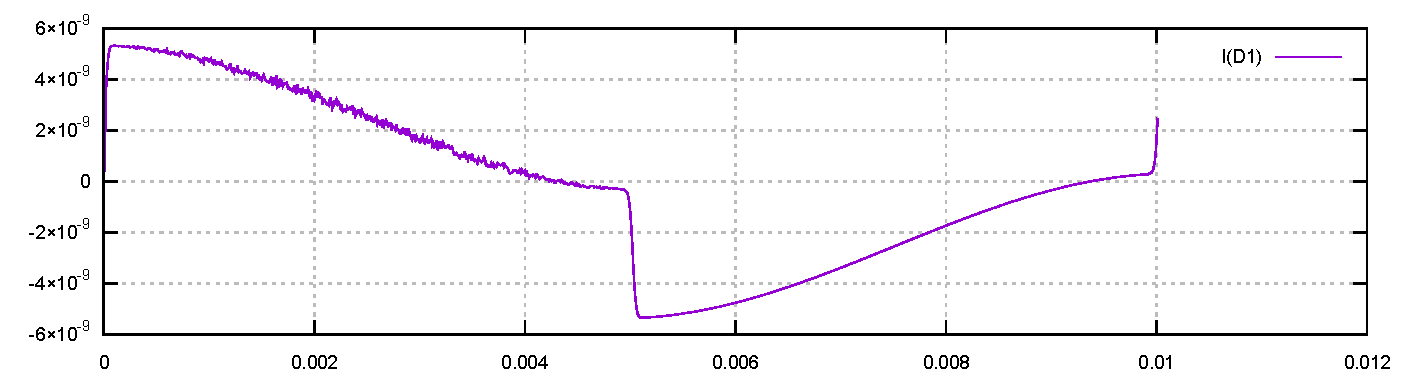
\includegraphics[width=0.9\linewidth]{backtoback-d}
		\caption*{double}
%	\end{subfigure}
%	\begin{subfigure}
		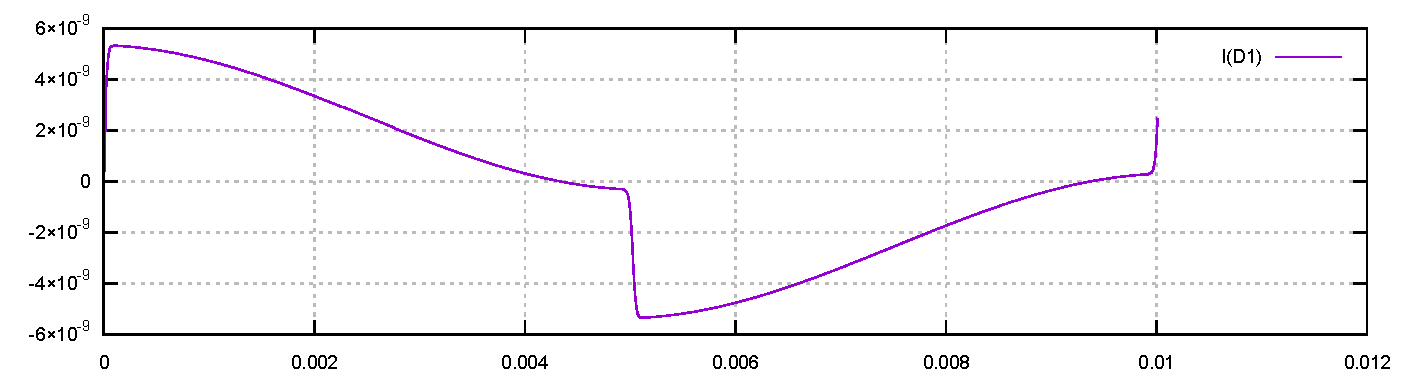
\includegraphics[width=0.9\linewidth]{backtoback-dd}
		\caption*{double-double}
%	\end{subfigure}
	\caption{Comparison of the simulation results for \texttt{backtoback} circuit for double and double-double precision type}
	\label{fig:results:noise}
\end{figure}

Nevertheless, the noise seems to be much smaller than the one produced when simulating the circuit with LTspice (see figure \ref{fig:back-to-back-circuit} back in the introduction chapter).

Using double-double precision over standard double precision helped solve convergence issues in many circuits and helped eliminate noise at the cost of slower simulation speed. From our observations, using quad-double over double-double does not bring any additional benefits (number of iterations needed to simulate the circuit stays the same, double-double already eliminates possible noise from truncation errors in the \texttt{backtoback} circuit) and only slows down the simulation by an order of magnitude. Therefore, we do not recommend using the quad-double type when using the NextGen SPICE library. Instead, we recommend using the double-double precision even though the simulation may be slower than when using only double precision.

In the future versions of the library, we would certainly like to add more convergence aids to ensure convergence even with double precision type. Then the choice of precision type would be based on whether the circuit is expected to be ill-conditioned or not.

\section{Comparison with Ngspice Simulator} 

Following table compares the simulation times of our library with the ngspice simulator. The times listed in the table were obtained using the \texttt{rusage trantime} command in ngspice interactive mode, which lists the time the simulator spent on the transient analysis in seconds with three decimal places. Because of the low resolution of the \texttt{trantime} information, we compared the runs only on the simulations which take several milliseconds. The ngspice simulator was run 5 times and the run times were averaged. The \texttt{adder} circuit was simulated for both 50 timesteps (as in previous section) and 6400 timesteps.

\begin{center}
	\begin{tabular}{|r|r|r|}
		\hline
		Circuit & ngspice & NextGen SPICE (double-double) \\ \hline \hline
		\texttt{cfflop} & 11 ms & 57 ms \\
		\texttt{rca3040} & 8 ms & 150 ms \\
		\texttt{sbdgate} & 6 ms & 130 ms \\
		\texttt{ua709} & 5 ms & 124 ms \\
		\texttt{adder} (50 ns) & 67 ms & 9,147 ms  \\
		\texttt{adder} (6400 ns) & 8.3 s & 898.1 s \\
		\hline
	\end{tabular}
\end{center}

The ngspice simulator is noticeably faster. The ratio of the runtimes of ngspice and that of our library seem roughly proportional to the number of variables in the equation system, in case of the \texttt{adder} circuit with 451 variables, the ngspice simulator was more than 100 times faster. We used the performance profiler integrated in Visual Studio 2017 to find out which parts of our simulator are the slowest. It turns out that the simulator spends more than 95\% of the time solving the equation system. The equation systems for the larger circuits are very sparse, in case of \texttt{adder} circuit, only around 1\% of the matrix entries are nonzero. Because our simulator uses full matrix representation, it spends too much time on multiplying and adding the zero entries. On the other hand, ngspice uses sparse matrix representation which performs only the necessary arithmetical operations.

Therefore, in the next versions of the library, we should implement the sparse matrix representation, and perhaps also consider using different method for solving the equation system to speed up the simulation. Possible choice would be using LU factorization which is also used by ngspice, or even iterative methods like Gauss-Seidel.

\section{Comparison with SpiceSharp}

NextGen SPICE is not the only circuit simulator library for .NET in development. There is SpiceSharp \cite{spicesharp}, whose development started shortly after that of our library. The SpiceSharp is made to resemble the original SPICE3F5, with some modifications to make the source code more appropriate for the .NET platform. Several parts of the source code contain comments with references to the original SPICE3's source and explanation how is it modified.

To compare the user interface of SpiceSharp with that of NextGen SPICE library, consider following code fragment for simulating the simple RLC circuit, which we have simulated in the NextGen SPICE tutorials back in section \ref{chap:tutorial-transient}. We omitted the declarations of outer class and namespace usings for brevity.

\begin{csharpcode}
private static void SpiceSharp()
{
	var circuit = new Circuit(
		new VoltageSource("V1", "1", "0",
			new Pulse(0, 5, 5e-3, 0, 0, 25e-3, double.MaxValue)),
		new Resistor("R1", "1", "2", 50),
		new Inductor("I1", "2", "3", 0.125),
		new Capacitor("C1", "3", "0", 1e-6)
	);
	
	Transient tran = new Transient("TRAN", 0.2e-3, 55e-3);
	Console.WriteLine("Time V(1) V(3) I(VC)");
	
	RealPropertyExport i_v1 = new RealPropertyExport(tran, "V1", "i");
	Console.WriteLine("Time V(1) V(3)");
	tran.OnExportSimulationData += (sender, args) =>
	{
		var time = args.Time;
		var v1 = args.GetVoltage("1");
		var v3 = args.GetVoltage("3");
		var i = i_v1.Value;
	
		Console.WriteLine($"{time} {v1} {v3} {i}");
	};
	
	tran.Run(circuit);
}
\end{csharpcode}

The SpiceSharp user interface is very similar to the SPICE netlist syntax. This means that all devices and nodes are identified by a string. In the NextGen SPICE library, the individual devices can be (optionally) tagged by an arbitrary C\# object.

Another difference is how a circuit is constructed, in case of simple devices, the identifiers of connected nodes are passed to the constructor, and the constructed devices can be passed to the \texttt{Circuit} class constructor. However, the connections for transistors can be only set by calling the \texttt{Connect} instance method, which we found counterintuitive. 

The individual simulations are done by calling a \texttt{Run} method on a dedicated simulation object with the simulated circuit as an argument (see lines 11 and 26 of the source above). Getting the simulation data is a bit tricky. The easiest way to get the node voltages in the individual timepoints is registering a handler on the \texttt{OnExportSimulationData} event (lines 14 to 20). To get e.g. current flowing through the voltage source, one has to use a \texttt{RealPropertyExport} class (line 14) and specify the name of the device and a string name of the property to be extracted. The value of this voltage source current can be then accessed via the \texttt{Value} property during the \texttt{OnExportSimulationData} callback (line 21). 

The SpiceSharp's interface makes heavy use of string values, in the example above we show that getting a current though a device requires knowledge of how the appropriate string identifier. What's worse, the strings are also used to set individual parameters for semiconductor devices. following code fragment is taken from the \texttt{SpiceSharpTest/Models/Semiconductors/DIO/DiodeTests.cs} file from the SpiceSharp's Github repository (version from 4th May 2018).

\begin{csharpcode}
     // Build circuit
	Circuit ckt = new Circuit();
	ckt.Objects.Add(
		CreateDiode("D1", "OUT", "0", "1N914", 
			"Is=2.52e-9 Rs=0.568 N=1.752 Cjo=4e-12 M=0.4 tt=20e-9"),
		new VoltageSource("V1", "OUT", "0", 0.0)
	);
\end{csharpcode}

The \texttt{CreateDiode} method is a helper method which parses the parameter string and sets individual parameters by calling \texttt{SetParameter} method on \texttt{Diode\+Model} class, which internally uses reflection to set appropriate property. The downside of this is that the parameter names cannot be hinted by automatic code completion feature of the IDE (like Intellisense in Visual Studio). These actual object on which the parameters are stored can be accessed, but it takes several casts and is by no means intuitive. Because of this, we consider the interface of our NextGen SPICE library superior to that of SpiceSharp.

Although it's interface is user unfriendly, SpiceSharp implements more circuit analyses and more circuit devices. Also, the implemented models for semiconductor devices are more detailed than those implemented in NextGen SPICE library. We would like to address this in the next version of our library and expand the set of implemented devices and add new analysis types.

We tried to compare the performance of SpiceSharp and the NextGen SPICE library. However, we have had difficulties parsing the netlist files containing the benchmark circuits in the SpiceSharp parser. Some netlist needed to be altered (e.g. \texttt{SIN} source changed to \texttt{SINE}, adding an argument with default value which is not strictly needed by SPICE3, or converting parts of the netlist to lowercase). The SpiceSharp simulator then reported a singular matrix when simulating the \texttt{adder} and \texttt{sbdgate} circuit, and in the circuits which were actually simulated, the SpiceSharp simulator used bigger timestep than we specified. This lead to very shorter simulation times and lower-resolution plots. This makes it difficult to compare the simulators performances. Following table lists measured times and number of timesteps computed.

\begin{center}
	\begin{longtable}{|l|r|r|r|r|r|}
		\hline
Method & Timepoints &        Mean &        Error &       StdDev & Scaled \\ \hline \hline
\multicolumn{6}{|l|}{\texttt{backtoback}} \\ \hline
NextGen SPICE &       1000 &    846.4 $\mu{}$s &    10.319 $\mu{}$s &     9.148 $\mu{}$s &   1.00 \\
SpiceSharp &       5550 & 69,987.3 $\mu{}$s &   565.747 $\mu{}$s &   472.424 $\mu{}$s &  82.70 \\ \hline \hline

\multicolumn{6}{|l|}{\texttt{cfflop}} \\ \hline
NextGen SPICE &       1000 & 59,352.3 $\mu{}$s & 1,151.949 $\mu{}$s & 1,232.573 $\mu{}$s &   1.00 \\
SpiceSharp &         81 &  2,051.9 $\mu{}$s &    29.520 $\mu{}$s &    27.613 $\mu{}$s &   0.03 \\ \hline \hline

\multicolumn{6}{|l|}{\texttt{choke}} \\ \hline
NextGen SPICE &        100 &  2,236.1 $\mu{}$s &    42.844 $\mu{}$s &    40.076 $\mu{}$s &   1.00 \\
SpiceSharp &         73 &    557.4 $\mu{}$s &     7.231 $\mu{}$s &     6.764 $\mu{}$s &   0.25 \\ \hline \hline

\multicolumn{6}{|l|}{\texttt{diffpair}} \\ \hline
NextGen SPICE &        100 &  8,576.7 $\mu{}$s &   165.504 $\mu{}$s &   215.202 $\mu{}$s &   1.00 \\
SpiceSharp &         59 &  1,032.8 $\mu{}$s &    10.943 $\mu{}$s &    10.236 $\mu{}$s &   0.12 \\  \hline \hline

\multicolumn{6}{|l|}{\texttt{rtlinv}} \\ \hline
NextGen SPICE &        100 &  1,569.9 $\mu{}$s &    13.843 $\mu{}$s &    12.271 $\mu{}$s &   1.00 \\
SpiceSharp &         80 &    988.7 $\mu{}$s &    10.505 $\mu{}$s &     9.826 $\mu{}$s &   0.63 \\ \hline \hline
	\end{longtable}
\end{center}

When comparing the runtimes per individual timepoint, the NextGen SPICE is around four times slower, which can be explained by the usage of double-double precision in NextGen SPICE and sparse matrix representation in SpiceSharp. However, when simulating te \texttt{backtoback} circuit, the SpiceSharp needed far more timepoint computations. As seen from in figure \ref{fig:backtoback-spicesharp}, the SpiceSharp does not correctly handle circuits with very small resistors.

\begin{figure}[h]
	\centering
	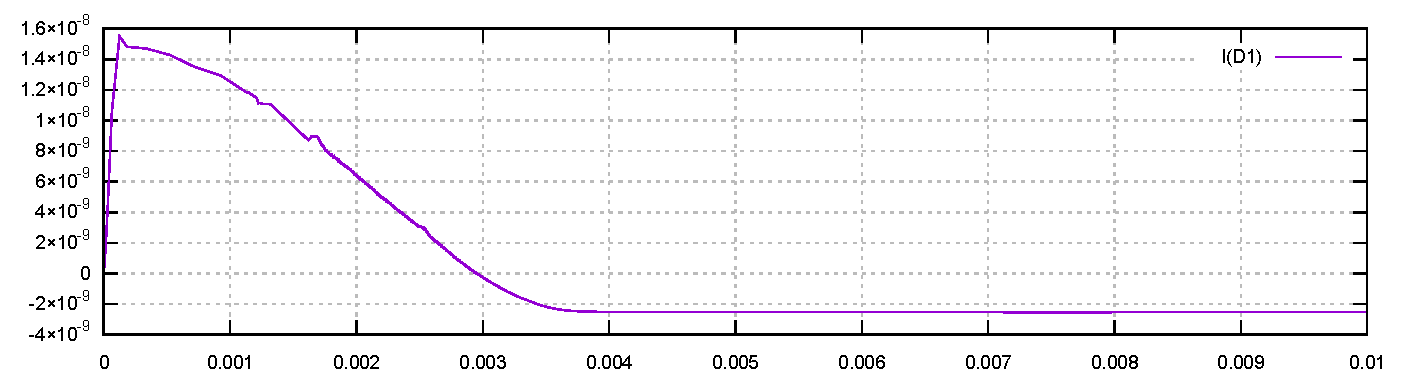
\includegraphics[width=0.9\linewidth]{backtoback-spicesharp.pdf}
	\caption{Plot of the \texttt{backtoback} circuit from SpiceSharp}
	\label{fig:backtoback-spicesharp}
\end{figure}

The plots of other circuits were similar to the ones produced by the NextGen SPICE, although the greater timestep resulted in visible straight regions in the plot. For example, figure \ref{fig:cfflop} shows plot of voltage in \texttt{cfflop} circuit on the \texttt{6} node. At $2\cdot 10^{-7}$ mark, the SpiceSharp output has visible straight edge. Also, the output our NextGen SPICE shows clearly the slight S shape of the slopes when voltage changes. This shape is not clearly visible on the SpiceSharp output.

\begin{figure}[h]
	\centering
	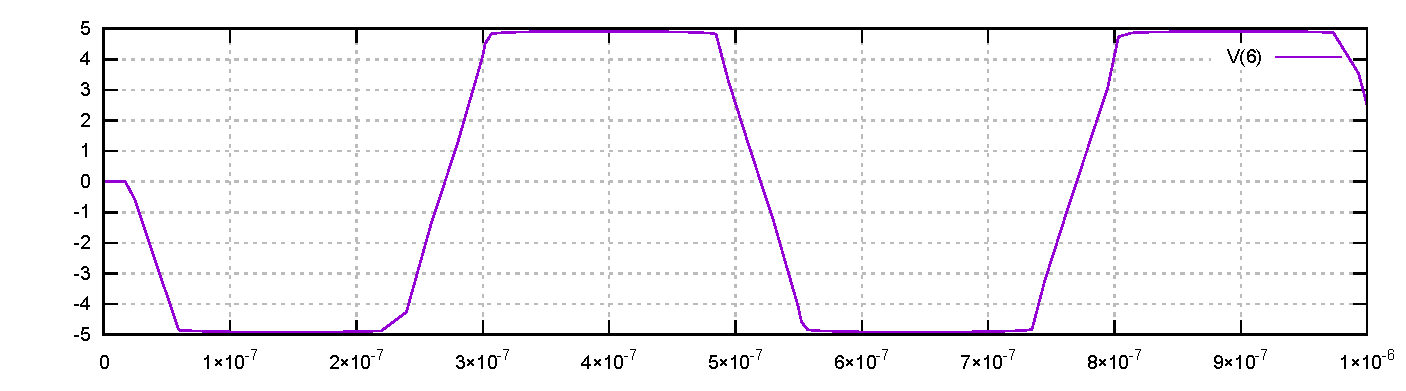
\includegraphics[width=0.9\linewidth]{cfflop-spicesharp}
	\caption*{SpiceSharp}
	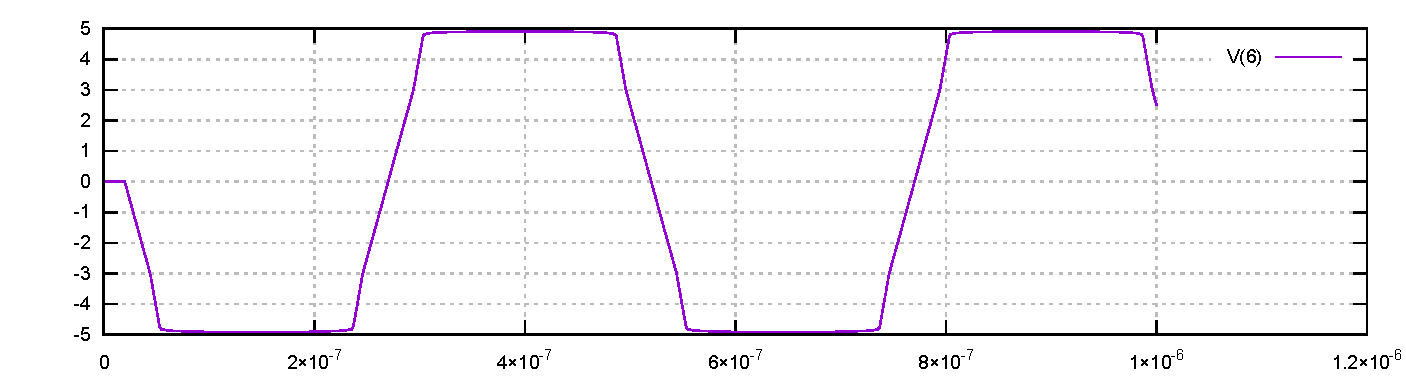
\includegraphics[width=0.9\linewidth]{cfflop}
	\caption*{NextGen SPICE}
	\caption{Comparison of simulation results on the \texttt{cfflop} circuit}
	\label{fig:cfflop}
\end{figure}

\section{Summary}

Considering the measurements listed in this chapter, the representation of equation system and method for solving it is crucial part of the circuit simulator. Our choice of the simplest implementation possible -- full matrix and Gaussian elimination -- caused our simulator to be orders of magnitude slower on large circuits than other circuit simulators. However, thanks to the abstraction we used during the implementation, more appropriate methods can be implemented in future versions of the library. 

In terms of the simulator output, NextGen SPICE produces visually same plots as other circuit simulators, and because of the double-double precision type used, it does not suffer from the noise caused by truncation error during equation system solution.

%%%%%%%%

%%%%%%%%

\chapter*{Conclusion}
\addcontentsline{toc}{chapter}{Conclusion}

To conclude our thesis, we will revisit the goals we set in the introduction chapter in section \ref{chap:intro:goals}

\begin{enumerate}
	\item \textit{Implement SPICE-like simulation library	}
	\begin{enumerate}
		\item \textit{Target .NET Standard for maximum portability} -- Our library requires .NET Standard 2.0, which makes it available on all major platforms running one of the newer version of .NET runtime.
		
		\item \textit{Support performing time-domain simulation of the circuit, and allow changing parameters of circuit devices between individual timesteps.} -- We designed our simulator in such a way that users of our library decide when next circuit state is computed and how big the timestep should be. Between the individual timesteps, users can modify parameters of the devices in the simulated circuit, and have the changes affect the next calculated circuit state. 
		
		\item \textit{Support following set of devices
		\begin{enumerate}
			\item Ideal resistor
			\item Ideal voltage source
			\item Ideal current source
			\item Ideal inductor
			\item Ideal capacitor
			\item SPICE diode
			\item SPICE BJT transistor
		\end{enumerate}}
		
		We successfully implemented all circuit devices listed above. In addition, we also implemented linear controlled sources: voltage controlled voltage source, voltage controlled current source, current controlled voltage source and current controlled current source.
		
		\item \textit{Allow new types of circuit analyses and circuit devices to be added to the simulator without modifying the library's source code.} -- We have written a guide on how to add new devices in library's user documentation in chapter \ref{chap:exteding} and provided an example of adding new device in section \ref{chap:userdocs:diode-tutorial}.
		
		\item \textit{Implement SPICE netlist parser to allow importing circuits and macromodels from standard SPICE netlist files.} -- Our parser supports sufficient subset of the SPICE3 netlist syntax to allow importing circuits and subcircuits (macromodels) containing devices implemented in our simulator. We have tested our parser on existing SPICE netlists with success. However, because the parser implementation present in the library implements only the data statements (devices, subcircuits and device models), it is necessary to remove any control statements from the netlist file before parsing them in NextGen SPICE.
		
		\item \textit{Allow users of the library to choose between double, double-double, and quad-double precision types and compare the library's performance with respect to speed and accuracy for each listed precision type.} -- Users can compile our library themselves and choose the precision type to be used by defining a certain conditional compilation symbol. We compared the simulator performance for each precision type and found out that the double-double type currently provides the best combination of convergence and simulation speed for our library.
	\end{enumerate}
	
	\item  \textit{Use the simulation library to implement SPICE-like console application for .NET Core, which would accept implemented subset of SPICE netlist syntax.} -- Our \texttt{NextGenSpice} application targets .NET Core 2.0 and provides the desired functionality by extending the library's parser to handle \texttt{.TRAN} \texttt{.OP} and \texttt{.PRINT} statements. We then used the library's functionality to run the simulations and print the requested data to standard output.
\end{enumerate}

\subsubsection{Future Work}
The NextGen SPICE library offers only a narrow subset of the SPICE-like simulators used today. Following list contains features which we consider most beneficial for the next version of the library.

\begin{itemize}
	\item \textit{Sparse matrix representation} -- As discussed in the \ref{chap:results-precision}, the Gauss-Jordan elimination and full matrix representation proved to be a performance bottleneck when simulating larger circuits. Using sparse matrix methods which are used by the standard SPICE implementations would significantly speed up the simulation.
	
	\item \textit{Dynamic timestep} -- Current implementation of the transient analysis algorithm relies on the user to choose a fixed timestep. As discussed in the analysis \ref{chap:analysis-timestep}, dynamic timestep mechanism can speedup simulation in regions where the capacitor charges and inductor fluxes do not change quickly.
	
	\item \textit{Implementing \texttt{.INCLUDE} statement} -- Currently all used models and subcircuits need to be defined in the netlist file. SPICE3's \texttt{.INCLUDE} statement works similarly to the \texttt{\#include} directive in C or C++ languages: the contents of the included file are treated as if they were copied and pasted in place of the \texttt{.INCLUDE} statement. This allows better reuse of the subcircuits and defined models.
	
	\item \textit{Interactive console application} -- Current \texttt{NextGenSpice} console application offers  limited interaction with the user. Also, when the user wants to run the same simulation with different parameters, the netlist file must be edited and the application run again. SPICE3 introduced an interactive mode, in which the program reads only the circuit description from the netlist file. The simulation statements and other control statements are then supplied on the standard input by the user.
	
	\item \textit{More devices and analysis types} -- Last but not least, the NextGen SPICE library as implemented in this thesis offers only a fraction of circuit analysis types and circuit devices. Examples of devices which are completely missing are switches (voltage and current controlled), other types of transistors (JFET, MOSFET), transmission lines, coupled inductors and semiconductor versions of resistor and capacitor devices. From the analysis types, the NextGenSpice library is missing e.g. the AC frequency sweep analysis, which requires small-signal models of the simulated devices.
\end{itemize}


%%% Bibliography
%%% Bibliography (literature used as a source)
%%%
%%% We employ bibTeX to construct the bibliography. It processes
%%% citations in the text (e.g., the \cite{...} macro) and looks up
%%% relevant entries in the bibliography.bib file.
%%%
%%% The \bibliographystyle command selects, which style will be used
%%% for references from the text. The argument in curly brackets is
%%% the name of the corresponding style file (*.bst). Both styles
%%% mentioned in this template are included in LaTeX distributions.

%\bibliographystyle{plainnat}    %% Author (year)
\bibliographystyle{unsrt}     %% [number]

\renewcommand{\bibname}{Bibliography}

%%% Generate the bibliography. Beware that if you cited no works,
%%% the empty list will be omitted completely.

\bibliography{bibliography}

%%% If case you prefer to write the bibliography manually (without bibTeX),
%%% you can use the following. Please follow the ISO 690 standard and
%%% citation conventions of your field of research.

% \begin{thebibliography}{99}
%
% \bibitem{lamport94}
%   {\sc Lamport,} Leslie.
%   \emph{\LaTeX: A Document Preparation System}.
%   2nd edition.
%   Massachusetts: Addison Wesley, 1994.
%   ISBN 0-201-52983-1.
%
% \end{thebibliography}


%%% Figures used in the thesis (consider if this is needed)
%\listoffigures

%%% Tables used in the thesis (consider if this is needed)
%%% In mathematical theses, it could be better to move the list of tables to the beginning of the thesis.
%\listoftables

%%% Abbreviations used in the thesis, if any, including their explanation
%%% In mathematical theses, it could be better to move the list of abbreviations to the beginning of the thesis.
%\chapwithtoc{List of Abbreviations}

%%% Attachments to the bachelor thesis, if any. Each attachment must be
%%% referred to at least once from the text of the thesis. Attachments
%%% are numbered.
%%%
%%% The printed version should preferably contain attachments, which can be
%%% read (additional tables and charts, supplementary text, examples of
%%% program output, etc.). The electronic version is more suited for attachments
%%% which will likely be used in an electronic form rather than read (program
%%% source code, data files, interactive charts, etc.). Electronic attachments
%%% should be uploaded to SIS and optionally also included in the thesis on a~CD/DVD.
%%% Allowed file formats are specified in provision of the rector no. 23/2016.
\chapwithtoc{Attachments}
\subsubsection{Contents of the attached CD}
\begin{itemize}
	\item \texttt{/sources} -- folder containing the \texttt{NextGenSpice} solution.
	\item \texttt{/examples} -- folder containing sample input files for the \texttt{NextGenSpice} standalone program.
	\item \texttt{/binaries} -- folder containing the binary files for the NextGen SPICE library and standalone console application, and \texttt{plot.ps1} Powershell script for running and automatically plotting the output data.
	\item \texttt{/references} -- folder containing copy of the documents which were the source for circuit simulation theory for this thesis.
	\subitem \texttt{/qucs.pdf} -- the QUCS Technical Papers \cite{qucs}
	\subitem \texttt{/ERL-520.pdf} -- Laurence W. Nagel's PhD thesis on SPICE2 \cite{Nagel:M520}
	\item \texttt{/documentation} -- folder containing the PDF version of the API reference for the NextGen SPICE simulator library.
	\item \texttt{/tex} -- folder containing the \LaTeX{} source for this thesis
	\subitem \texttt{/en} -- folder with the \texttt{.tex} files
	\subitem \texttt{/img} -- folder with images used in this thesis
	\subitem \texttt{/LICENSE.TXT} -- file containing licensing information
	\item \texttt{/thesis.pdf} -- file containing this thesis.
	\item \texttt{/README.txt} -- file describing the contents of the CD.
\end{itemize}

\openright
\end{document}
